\begin{componente}{CLIPS}
\compDescrizione{package generale contenente il prodotto del progetto}
\begin{compPackageContenuti}
\item \texttt{CLIPS::client}: componente globale per il front end del prodotto che utilizza il design pattern \gl{MVC}. Si occupa di fornire un'interfaccia grafica dell'applicazione e di interagire con il lato server.
\item \texttt{CLIPS::server}: componente globale per il back end del prodotto
\end{compPackageContenuti}
\end{componente}
\begin{componente}{CLIPS::client}
\begin{figure}[h!]
\centering
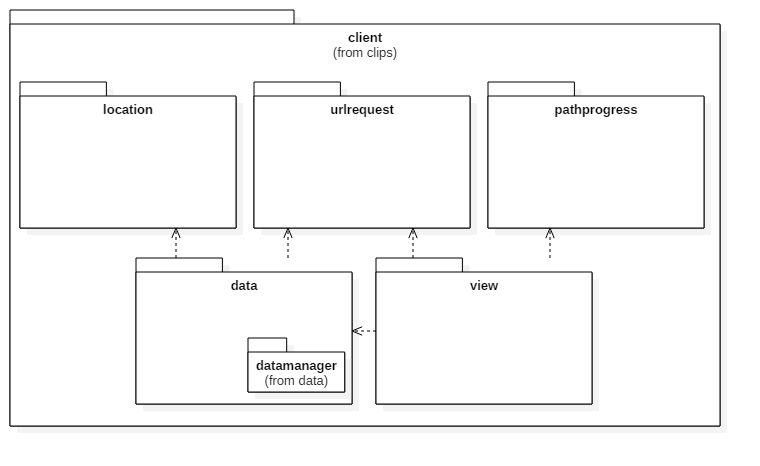
\includegraphics[scale=0.4]{img/package/png/client.png}
\caption{Schema package client}
 \end{figure}
\compDescrizione{componente globale per il front end del prodotto che utilizza il design pattern \gl{MVC}. Si occupa di fornire un'interfaccia grafica dell'applicazione e di interagire con il lato server.}
\compPadre{CLIPS}
\begin{compPackageContenuti}
\item \texttt{CLIPS::client::data}: package per la gestione in locale dei dati
\item \texttt{CLIPS::client::pathprogress}: componente che gestisce i dati del percorso e salva i risultati ottenuti nelle prove mentre si sta giocando
\item \texttt{CLIPS::client::viewcontroller}: componente che raggruppa tutte le view ed i controller relativi alle view
\end{compPackageContenuti}
\end{componente}
\begin{componente}{CLIPS::client::data}
\begin{figure}[h!]
	\centering
	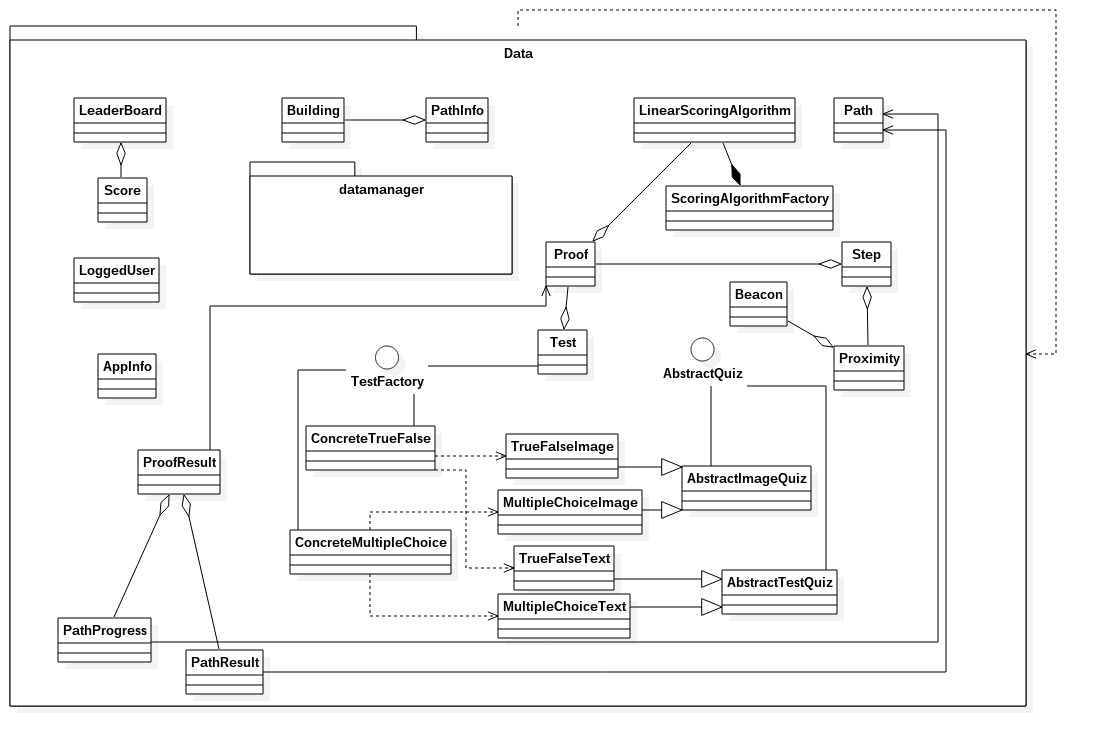
\includegraphics[scale=0.35]{img/package/png/client--data--min.png}
	\caption{Schema sintetico package client::data}
\end{figure}
\begin{figure}[h!]
	\centering
	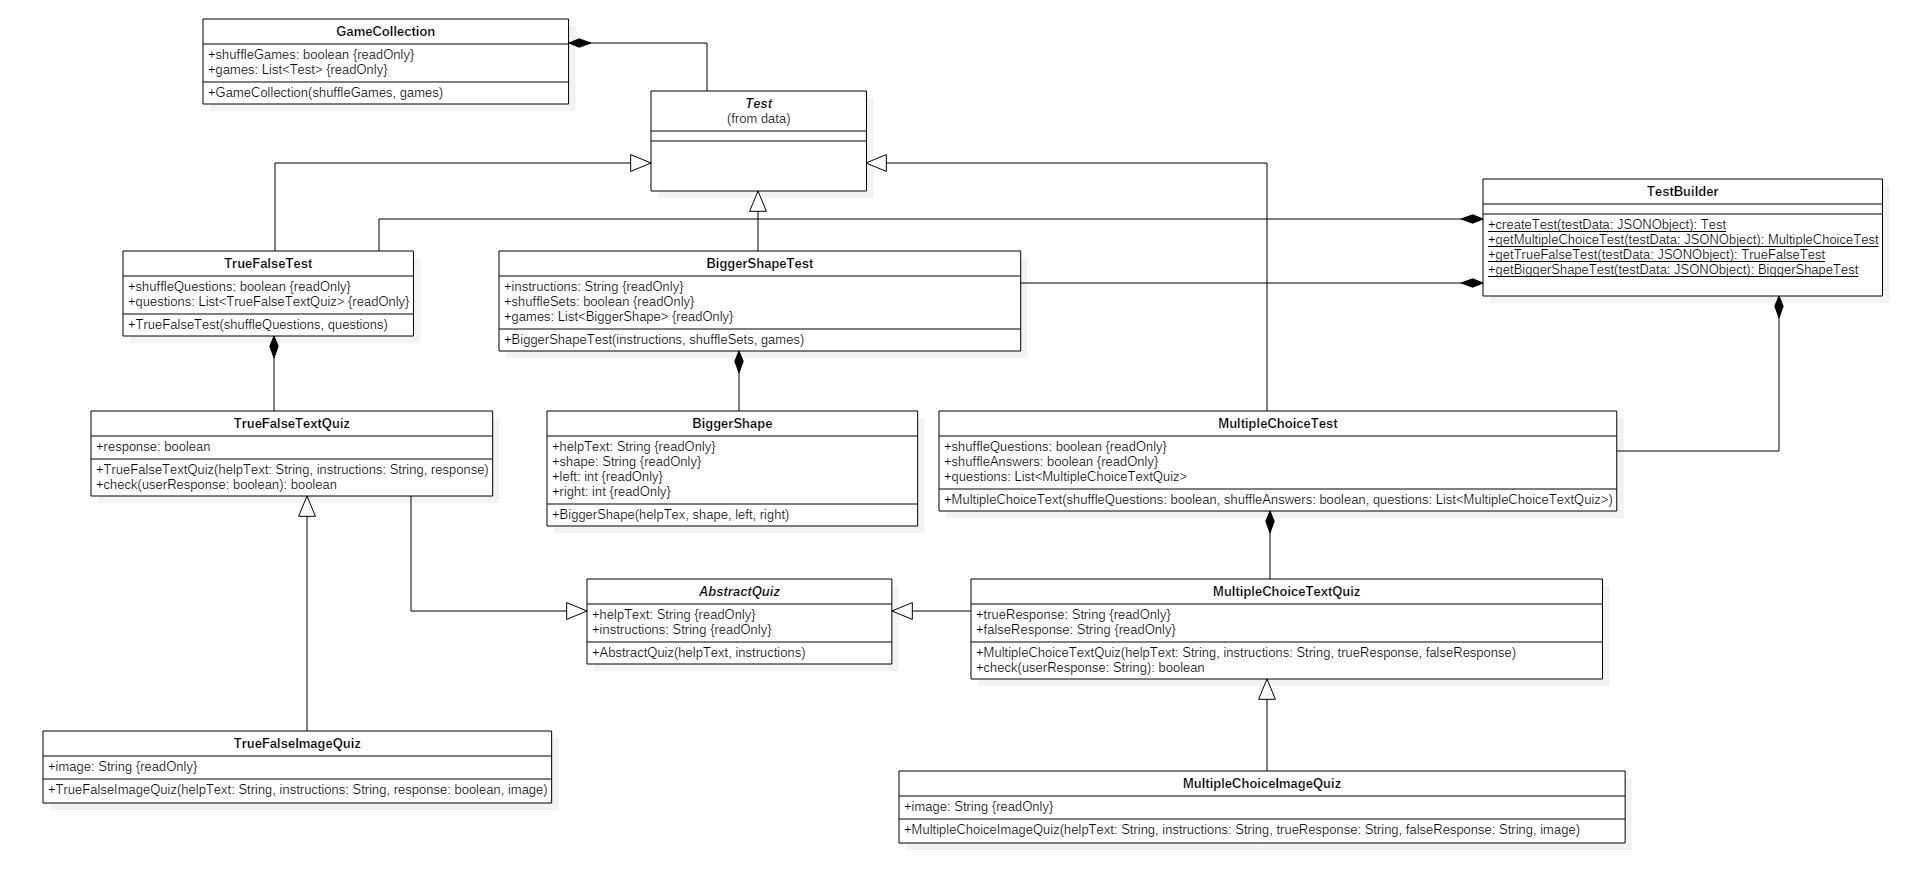
\includegraphics[scale=0.35]{img/package/png/client--data1.png}
	\caption{Prima parte schema package client::data}
\end{figure}
\begin{figure}[h!]
	\centering
	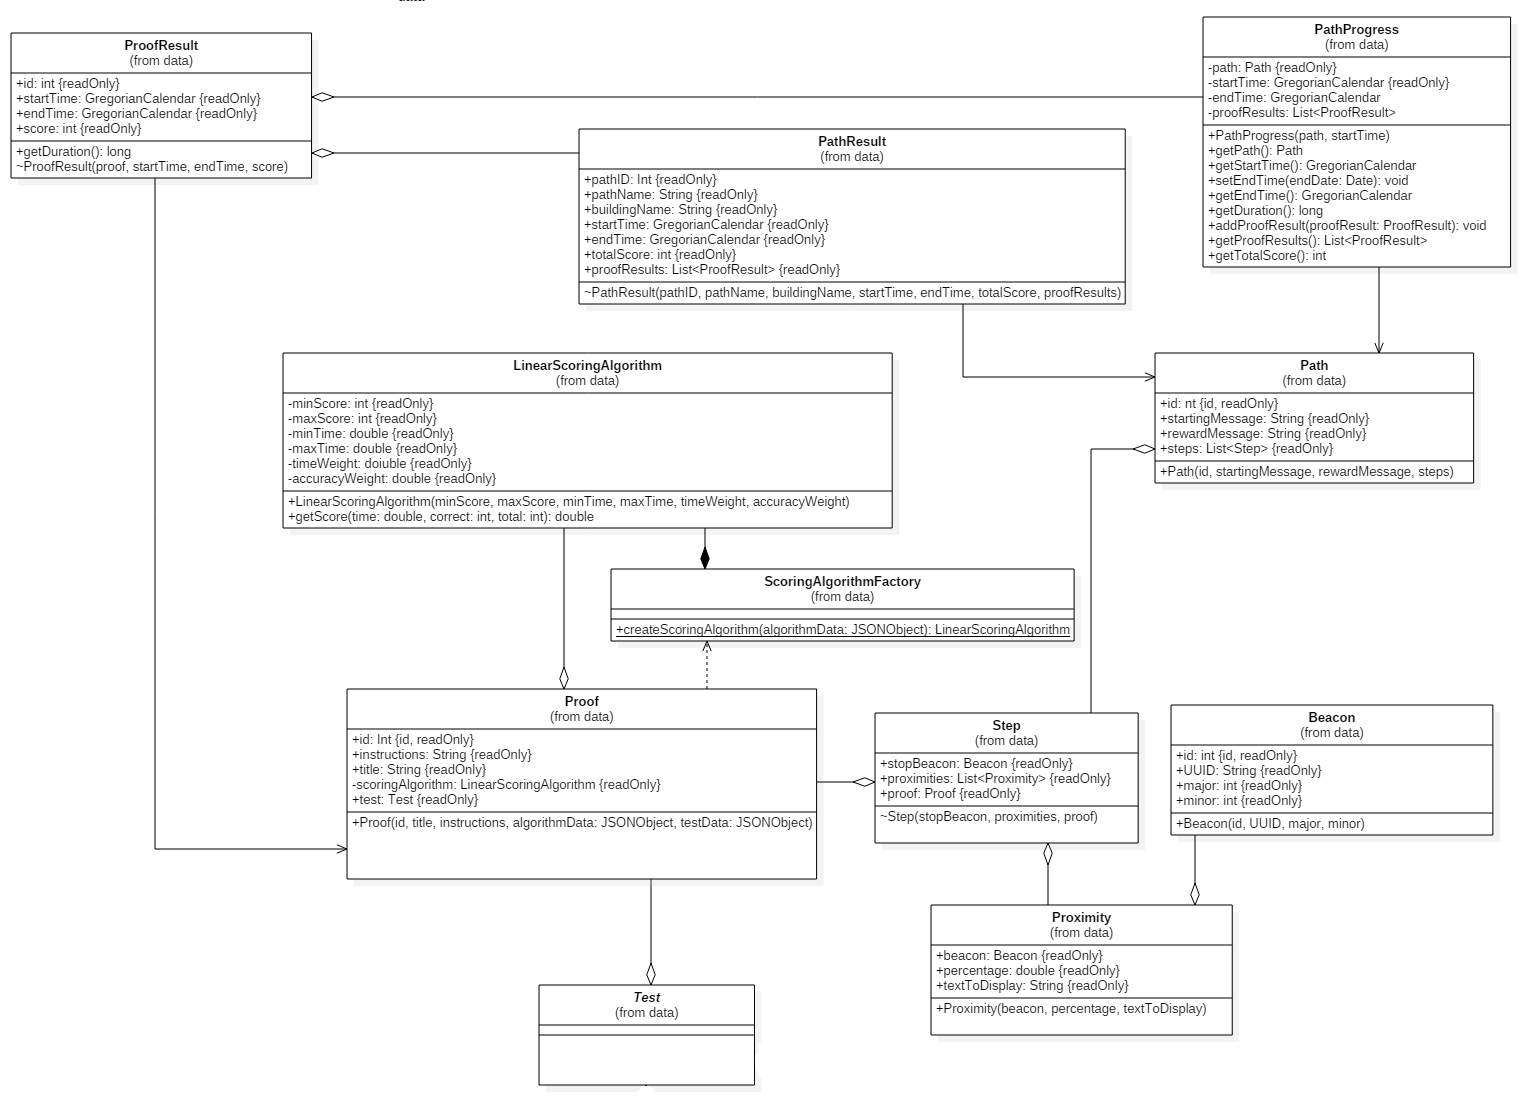
\includegraphics[scale=0.35]{img/package/png/client--data2.png}
	\caption{Seconda parte schema package client::data}
\end{figure}
\begin{figure}[h!]
	\centering
	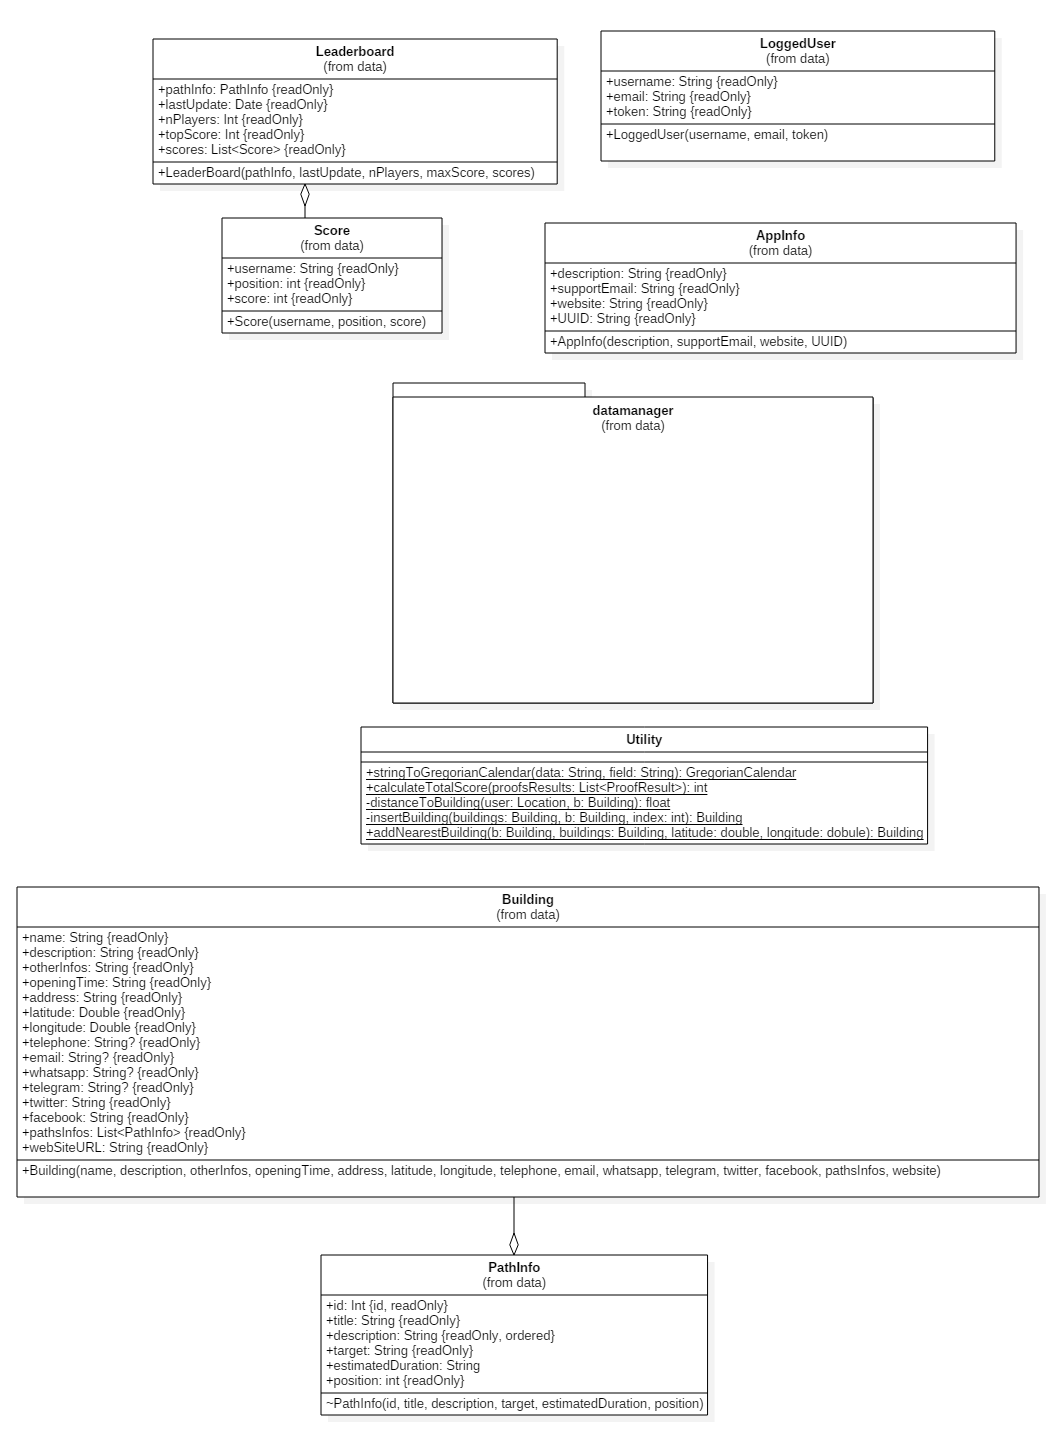
\includegraphics[scale=0.4]{img/package/png/client--data3.png}
	\caption{Terza parte schema package client::data}
\end{figure}
\compDescrizione{package per la gestione in locale dei dati}
\compPadre{client}
\begin{compPackageContenuti}
\item \texttt{CLIPS::client::data::datamanager}: componente che gestisce i dati in locale
\item \texttt{CLIPS::client::data::urlrequest}: componente che si occupa di effettuare le richieste al server
\end{compPackageContenuti}
\begin{compClassi} \\
\begin{classe}{CLIPS::client::data::\textit{AbstractQuiz}}
\classeDescrizione{classe astratta dei quiz}
\classeUtilizzo{classe astratta da cui far derivare tutte le classi che rappresentano un quiz}
\begin{classeAttributi}
\classeAttributo{helpText}{string}{stringa contenente il messaggio d'aiuto per la prova}
\classeAttributo{instructions}{string}{stringa contenente le istruzioni della prova}
\end{classeAttributi}
\end{classe}\begin{classe}{CLIPS::client::data::\textit{Test}}
\classeDescrizione{classe astratta che rappresenta un test}
\classeUtilizzo{classe astratta per rappresentare un test, ovvero un gruppo di giochi generalmente dello stesso tipo}
\end{classe}\begin{classe}{CLIPS::client::data::AppInfo}
\classeDescrizione{classe per la rappresentazione delle informazioni dell'applicazione}
\classeUtilizzo{permette di salvare le informazioni generali relative all'applicazione}
\begin{classeAttributi}
\classeAttributo{description}{string}{stringa contenente la descrizione dell'applicazione}
\classeAttributo{supportEmail}{string}{stringa contenente l'email per l'assistenza}
\classeAttributo{UUID}{string}{stringa contenente l'UUID utilizzato dai beacon dell'applicazione}
\classeAttributo{website}{string}{stringa contenente il sito dell'applicazione}
\end{classeAttributi}
\end{classe}\begin{classe}{CLIPS::client::data::Beacon}
\classeDescrizione{classe che rappresenta un beacon in locale}
\classeUtilizzo{permette di salvere in locale le informazioni di un beacon}
\begin{classeAttributi}
\classeAttributo{id}{int}{rappresenta il codice identificativo}
\classeAttributo{major}{int}{rappresenta il parametro major di un beacon}
\classeAttributo{minor}{int}{rappresenta il parametro minor di un beacon}
\classeAttributo{UUID}{string}{rappresenta il codice UUID di un beacon}
\end{classeAttributi}
\begin{classeMetodi}
\classeMetodo{Beacon(id:int,UUID:string,major:int,minor:int)}{id, major, minor, UUID}{void}{costruttore della classe beacon}
\begin{classeMetodoArgomenti}
\classeMetodoArgomento{id}{int}{codice identificativo}
\classeMetodoArgomento{major}{int}{parametro major del beacon}
\classeMetodoArgomento{minor}{int}{parametro minor del beacon}
\classeMetodoArgomento{UUID}{string}{codice UUID}
\end{classeMetodoArgomenti}
\end{classeMetodi}
\end{classe}\begin{classe}{CLIPS::client::data::BiggerShape}
\classeDescrizione{classe che rappresenta un gioco in cui bisogna selezionare la figura più grande tra le due che appaiono}
\classeUtilizzo{classe per rappresentare un gioco in cui l'utente deve selezionare la figura più grande tra le due che compaiono}
\begin{classeAttributi}
\classeAttributo{helpText}{string}{stringa contenente il messaggio d'aiuto per la prova}
\classeAttributo{left}{int}{intero contenente l'indice della figura rappresentata a sinistra}
\classeAttributo{right}{int}{intero contenente l'indice della figura rappresentata a destra}
\classeAttributo{shape}{string}{stringa contenente il tipo di figura rappresentata}
\end{classeAttributi}
\end{classe}\begin{classe}{CLIPS::client::data::BiggerShapeTest}
\classeDescrizione{classe che rappresenta un test di BiggerShape}
\classeUtilizzo{classe per rappresentare un test di BiggerShape}
\begin{classeAttributi}
\classeAttributo{games}{List<BiggerShape>}{lista contenente i quesiti proposti}
\classeAttributo{instructions}{string}{stringa contenente le istruzioni della prova}
\classeAttributo{shuffleSets}{boolean}{booleano per indicare se la lista dei quesiti va mescolata o meno}
\end{classeAttributi}
\begin{classeRelazioni}
\classeRelazione{CLIPS::client::data}{BiggerShape}{classe che rappresenta un gioco in cui bisogna selezionare la figura più grande tra le due che appaiono}\end{classeRelazioni}
\end{classe}\begin{classe}{CLIPS::client::data::Building}
\classeDescrizione{classe che rappresenta un edificio}
\classeUtilizzo{permette di memorizzare i dati di un edificio in locale}
\begin{classeAttributi}
\classeAttributo{address}{string}{indica l'indirizzo dell'edificio}
\classeAttributo{description}{string}{rappresenta una breve descrizione dell'edificio}
\classeAttributo{email}{string}{rappresenta l'indirizzo email dell'edificio}
\classeAttributo{facebook}{string}{indica l'indirizzo facebook dell'edificio}
\classeAttributo{id}{int}{identifica l'edificio univocamente}
\classeAttributo{latitude}{double}{rappresenta la latitudine dell'edificio}
\classeAttributo{longitude}{double}{rappresenta la longitudine dell'edificio}
\classeAttributo{name}{string}{indica il nome dell'edificio}
\classeAttributo{openingTime}{string}{rappresenta gli orari di apertura dell'edificio}
\classeAttributo{otherInfos}{string}{contiene informazioni aggiuntive sull'edificio}
\classeAttributo{pathsInfos}{string}{fornisce informazioni sui percorsi dell'edificio}
\classeAttributo{telegram}{string}{rappresenta il contatto telegram dell'edificio}
\classeAttributo{telephone}{string}{indica il numero di telefono dell'edificio}
\classeAttributo{twitter}{string}{rappresenta l'indirizzo twitter dell'edificio}
\classeAttributo{webSiteURL}{string}{indica l'indirizzo web dell'edificio}
\classeAttributo{whatsapp}{string}{indica il contatto whatsapp dell'edificio}
\end{classeAttributi}
\begin{classeRelazioni}
\classeRelazione{CLIPS::client::data}{PathInfo}{classe che si occupa di salvare in locale le informazioni generali di un percorso}\end{classeRelazioni}
\end{classe}\begin{classe}{CLIPS::client::data::GameCollection}
\classeDescrizione{classe che rappresenta un insieme di test}
\classeUtilizzo{classe per rappresentare un test in cui sono contenuti più tipi di giochi, di fatto è un test che contiene altri test}
\begin{classeAttributi}
\classeAttributo{games}{List<Test>}{lista contenente i test da proporre}
\classeAttributo{shuffleGames}{boolean}{booleano per indicare se la lista dei Test va mescolata o meno}
\end{classeAttributi}
\begin{classeRelazioni}
\classeRelazione{CLIPS::client::data}{\textit{Test}}{classe astratta che rappresenta un test}\end{classeRelazioni}
\end{classe}\begin{classe}{CLIPS::client::data::LeaderBoard}
\classeDescrizione{classe che rappresenta la classifica di un percorso}
\classeUtilizzo{consente di salvare i dati della classifica in locale}
\begin{classeAttributi}
\classeAttributo{lastUpdate}{DataManager}{data contenente la data dell'ultimo aggiornamento}
\classeAttributo{maxScore}{int}{intero contenente lo Score massimo raggiunto nella Leaderboard}
\classeAttributo{nPlayers}{int}{intero contenente il numero di giocatori nella Leaderboard}
\classeAttributo{pathInfo}{PathInfo}{oggetto PathInfo di cui registrare i record}
\classeAttributo{scores}{List<Score>}{lista contenente gli Score da mostrare nella Leaderboard}
\end{classeAttributi}
\begin{classeRelazioni}
\classeRelazione{CLIPS::client::data}{PathInfo}{classe che si occupa di salvare in locale le informazioni generali di un percorso}\classeRelazione{CLIPS::client::data}{Score}{classe che rappresenta il risultato nella classifica dell'utente}\end{classeRelazioni}
\end{classe}\begin{classe}{CLIPS::client::data::LinearScoringAlgorithm}
\classeDescrizione{classe per calcolare il punteggio di una prova. Per approfondire si veda \hyperref[sec:Algoritmo di assegnazione del punteggio]{Algoritmo di Assegnazione del Punteggio}}
\classeUtilizzo{si occupa di calcolare il punteggio utilizzando un algoritmo lineare}
\begin{classeAttributi}
\classeAttributo{accuracyWeight}{double}{indica l'incidenza dell'accuratezza rispetto alla risposta}
\classeAttributo{maxScore}{int}{indica il punteggio massimo}
\classeAttributo{maxTime}{double}{indica il tempo massimo}
\classeAttributo{minScore}{int}{indica il punteggio minimo}
\classeAttributo{minTime}{double}{indica il tempo minimo}
\classeAttributo{timeWeight}{double}{indica l'incidenza del tempo nel calcolo del punteggio}
\end{classeAttributi}
\begin{classeMetodi}
\classeMetodo{getScore}{correct, total}{int}{fornisce il punteggio ottenuto nella prova}
\begin{classeMetodoArgomenti}
\classeMetodoArgomento{correct}{int}{indica il numero di risposte corrette}
\classeMetodoArgomento{total}{int}{indica il numero totale di risposte fornite}
\end{classeMetodoArgomenti}
\end{classeMetodi}
\end{classe}\begin{classe}{CLIPS::client::data::LoggedUser}
\classeDescrizione{classe che si occupa di memorizzare in locale i dati dell'utente loggato}
\classeUtilizzo{permette il salvataggio in locale dei dati di un utente loggato}
\begin{classeAttributi}
\classeAttributo{email}{string}{stringa contenente l'email dell'utente che ha fatto il login}
\classeAttributo{token}{string}{stringa contenente il token di autenticazione dell'utente che ha fatto il login}
\classeAttributo{username}{string}{stringa contenente lo username dell'utente che ha fatto il login}
\end{classeAttributi}
\end{classe}\begin{classe}{CLIPS::client::data::MultipleChoiceImageQuiz}
\classeDescrizione{classe che rappresenta una domanda a risposta multipla con immagine}
\classeUtilizzo{classe per rappresentare una domanda a risposta multipla in cui viene usata un'immagine per la formulazione del quesito}
\begin{classeAttributi}
\classeAttributo{image}{string}{stringa contenente il nome dell'immagine}
\end{classeAttributi}
\end{classe}\begin{classe}{CLIPS::client::data::MultipleChoiceTest}
\classeDescrizione{classe che rappresenta un test di domande a risposta multiple}
\classeUtilizzo{classe per rappresentare un test di domande a risposta multipla, con immagine o senza}
\begin{classeAttributi}
\classeAttributo{questions}{List<MultipleChoiceTextQuiz>}{lista contenente i quesiti proposti}
\classeAttributo{shuffleAnswers}{boolean}{booleano per indicare se le risposte vanno mescolate o meno}
\classeAttributo{shuffleQuestions}{boolean}{booleano per indicare se le domande vanno mescolate o meno}
\end{classeAttributi}
\begin{classeRelazioni}
\classeRelazione{CLIPS::client::data}{MultipleChoiceTextQuiz}{classe che rappresenta una domanda a risposta multipla}\end{classeRelazioni}
\end{classe}\begin{classe}{CLIPS::client::data::MultipleChoiceTextQuiz}
\classeDescrizione{classe che rappresenta una domanda a risposta multipla}
\classeUtilizzo{classe per rappresentare una domanda a risposta multipla il cui contenuto è solo testo}
\begin{classeAttributi}
\classeAttributo{falseResponse}{string}{array contenente le risposte errate}
\classeAttributo{trueResponse}{string}{stringa contenente la risposta corretta}
\end{classeAttributi}
\begin{classeMetodi}
\classeMetodo{check}{userResponse}{boolean}{metodo per controllare se la risposta data dall'utente è quella corretta o meno}
\begin{classeMetodoArgomenti}
\classeMetodoArgomento{userResponse}{string}{stringa contenente la risposta data dall'utente}
\end{classeMetodoArgomenti}
\end{classeMetodi}
\end{classe}\begin{classe}{CLIPS::client::data::Path}
\classeDescrizione{classe che si occupa di salvare in locale i dati riguardanti un percorso}
\classeUtilizzo{permette di salvare i dati di un percorso in locale}
\begin{classeAttributi}
\classeAttributo{id}{int}{intero contenente l'id dell'oggetto}
\classeAttributo{rewardMessage}{string}{stringa contenente il messaggio che appare quando si completa il percorso}
\classeAttributo{startingMessage}{string}{stringa contenente il messaggio che appare quando si comincia il percorso}
\classeAttributo{steps}{List<Step>}{lista contenente gli step del percorso}
\end{classeAttributi}
\begin{classeRelazioni}
\classeRelazione{CLIPS::client::data}{Step}{classe che rappresenta in locale lo spostamento da una prova a quella successiva}\end{classeRelazioni}
\end{classe}\begin{classe}{CLIPS::client::data::PathInfo}
\classeDescrizione{classe che si occupa di salvare in locale le informazioni generali di un percorso}
\classeUtilizzo{consente di salvare in locale le informazioni generali di un percorso}
\begin{classeAttributi}
\classeAttributo{description}{string}{stringa contenente la descrizione del percorso}
\classeAttributo{estimatedDuration}{string}{stringa contenente la durata stimata del percorso}
\classeAttributo{id}{int}{intero contenente l'id dell'oggetto}
\classeAttributo{target}{string}{stringa per indicare a chi è consigliato il percorso}
\classeAttributo{title}{string}{stringa contenente il titolo del percorso}
\end{classeAttributi}
\end{classe}\begin{classe}{CLIPS::client::data::PathProgress}
\classeDescrizione{classe per il salvataggio in locale del progresso di un percorso}
\classeUtilizzo{permette di salvare in locale i risultati delle prove durante lo svolgimento del percorso}
\begin{classeAttributi}
\classeAttributo{endTime}{GregorianCalendar}{oggetto contenente la data e l'orario in cui l'utente ha completato il percorso}
\classeAttributo{path}{Path}{oggetto Path di cui tenere traccia del progresso dell'utente}
\classeAttributo{proofResults}{List<Building>}{lista contenente i risultati delle prove completate dall'utente}
\classeAttributo{startTime}{GregorianCalendar}{oggetto contenente la data e l'orario in cui l'utente ha cominciato il percorso}
\end{classeAttributi}
\begin{classeMetodi}
\classeMetodo{addProofResult}{proofResult}{void}{metodo per aggiungere il risultato di una Proof completata dall'utente alla lista proofResults}
\begin{classeMetodoArgomenti}
\classeMetodoArgomento{proofResult}{ProofResult}{oggetto contenente i  risultati della prova completata dall'utente}
\end{classeMetodoArgomenti}
\classeMetodo{getDuration}{}{long}{metodo per ottenere la durata del percorso svolto dall'utente}
\classeMetodo{getEndTime}{}{GregorianCalendar}{metodo per ottenere l'oggetto contenente la data e l'orario in cui si è completato il percorso}
\classeMetodo{getPath}{}{Path}{metodo per ottenere l'oggetto Path a cui si riferisce l'oggetto PathProgress}
\classeMetodo{getProofResults}{}{List<Building>}{metodo per ottenere la lista dei risultati delle Proof completate dall'utente}
\classeMetodo{getStartTime}{}{GregorianCalendar}{metodo per ottenere l'oggetto contenente la data e l'orario in cui si è cominciato il percorso}
\classeMetodo{getTotalScore}{}{int}{metodo per calcolare lo Score totale ottenuto dall'utente nel percorso svolto}
\classeMetodo{setEndTime}{endTime}{void}{metodo per impostare data e orario di quando l'utente ha completato il percorso}
\begin{classeMetodoArgomenti}
\classeMetodoArgomento{endTime}{GregorianCalendar}{oggetto contenente la data e l'orario in cui l'utente ha completato il percorso}
\end{classeMetodoArgomenti}
\end{classeMetodi}
\begin{classeRelazioni}
\classeRelazione{CLIPS::client::data}{Path}{classe che si occupa di salvare in locale i dati riguardanti un percorso}\classeRelazione{CLIPS::client::data}{ProofResult}{classe che rappresenta il risultato di una prova}\end{classeRelazioni}
\end{classe}\begin{classe}{CLIPS::client::data::PathResult}
\classeDescrizione{classe che rappresenta i risultati di un percorso}
\classeUtilizzo{permette di salvare i dati di un percorso in locale}
\begin{classeAttributi}
\classeAttributo{buildingName}{string}{stringa contenente il nome dell'edificio in cui si trova il percorso}
\classeAttributo{endTime}{GregorianCalendar}{oggetto contenente la data e l'orario in cui l'utente ha completato il percorso}
\classeAttributo{pathID}{int}{intero contenente l'id del Patha cui si riferisce l'oggetto}
\classeAttributo{pathName}{string}{stringa contenente il nome del percorso}
\classeAttributo{proofResults}{List<ProofResult>}{lista contenente i risultati delle prove del percorso completate dall'utente}
\classeAttributo{startTime}{GregorianCalendar}{oggetto contenente la data e l'orario in cui l'utente ha cominciato il percorso}
\classeAttributo{totalScore}{int}{intero contenente lo Score totale del percorso ottenuto dall'utente}
\end{classeAttributi}
\begin{classeRelazioni}
\classeRelazione{CLIPS::client::data}{ProofResult}{classe che rappresenta il risultato di una prova}\end{classeRelazioni}
\end{classe}\begin{classe}{CLIPS::client::data::Proof}
\classeDescrizione{classe che rappresenta una prova del percorso}
\classeUtilizzo{salva in locale i dati della prova da far visualizzare all'utente}
\begin{classeAttributi}
\classeAttributo{id}{int}{intero contenente l'id dell'oggetto}
\classeAttributo{instructions}{string}{stringa contenente le istruzioni della prova}
\classeAttributo{scoringAlgorithm}{LinearScoringAlgorithm}{oggetto contenente l'algoritmo per calcolare il punteggio della prova}
\classeAttributo{test}{Test}{oggetto contenente il quesito da proporre all'utente}
\classeAttributo{title}{string}{stringa contenente il titolo della prova}
\end{classeAttributi}
\begin{classeRelazioni}
\classeRelazione{CLIPS::client::data}{\textit{Test}}{classe astratta che rappresenta un test}\classeRelazione{CLIPS::client::data}{LinearScoringAlgorithm}{classe per calcolare il punteggio di una prova}\classeRelazione{CLIPS::client::data}{ScoringAlgorithmFactory}{classe base per la creazione degli algoritmi}\end{classeRelazioni}
\end{classe}\begin{classe}{CLIPS::client::data::ProofResult}
\classeDescrizione{classe che rappresenta il risultato di una prova}
\classeUtilizzo{permette di salvare in locale il risultato di una prova}
\begin{classeAttributi}
\classeAttributo{endTime}{GregorianCalendar}{oggetto contenente la data e l'orario in cui l'utente ha completato il percorso}
\classeAttributo{id}{int}{intero contenente l'id dell'oggetto}
\classeAttributo{score}{int}{intero contenente il punteggio ottenuto dall'utente}
\classeAttributo{startTime}{GregorianCalendar}{oggetto contenente la data e l'orario in cui l'utente ha cominciato il percorso}
\end{classeAttributi}
\begin{classeMetodi}
\classeMetodo{getDuration}{}{long}{metodo per ottenere la durata della prova svolta dall'utente}
\end{classeMetodi}
\begin{classeRelazioni}
\classeRelazione{CLIPS::client::data}{PathProgress}{classe per il salvataggio in locale del progresso di un percorso}\classeRelazione{CLIPS::client::data}{PathResult}{classe che rappresenta i risultati di un percorso}\classeRelazione{CLIPS::client::data}{Proof}{classe che rappresenta una prova del percorso}\end{classeRelazioni}
\end{classe}\begin{classe}{CLIPS::client::data::Proximity}
\classeDescrizione{classe che rappresenta in locale un beacon indicato alla segnalazione della distanza dalla prossima prova}
\classeUtilizzo{consente di salvare un beacon e la sua distanza dal beacon della prossima prova}
\begin{classeAttributi}
\classeAttributo{beacon}{Beacon}{oggetto Beacon a cui fa riferimento l'oggetto}
\classeAttributo{percentage}{double}{rappresenta la distanza dell'utente dal Beacon in percentuale}
\classeAttributo{textToDisplay}{string}{stringa contenente il testo da mostrare all'utente quando si avvicina al Beacon}
\end{classeAttributi}
\begin{classeRelazioni}
\classeRelazione{CLIPS::client::data}{Beacon}{classe che rappresenta un beacon in locale}\end{classeRelazioni}
\end{classe}\begin{classe}{CLIPS::client::data::Score}
\classeDescrizione{classe che rappresenta il risultato nella classifica dell'utente}
\classeUtilizzo{permette di memorizzare il punteggio e la posizione in classifica dell'utente}
\begin{classeAttributi}
\classeAttributo{position}{int}{intero contenente la posizione dello Score nella schermata}
\classeAttributo{score}{int}{intero contenente il punteggio ottenuto dall'utente}
\classeAttributo{username}{string}{stringa contenente lo username dell'utente che ha ottenuto il punteggio}
\end{classeAttributi}
\end{classe}\begin{classe}{CLIPS::client::data::ScoringAlgorithmFactory}
\classeDescrizione{classe base per la creazione degli algoritmi}
\classeUtilizzo{fornisce il metodo per la creazione di algoritmi per il calcolo dei punteggi}
\begin{classeMetodi}
\classeMetodo{createScoringAlgorithm}{algorithmData}{void}{si occupa di creare l'algoritmo per calcolare il punteggio}
\begin{classeMetodoArgomenti}
\classeMetodoArgomento{algorithmData}{void}{JSON contenente i dati necessari alla creazione di un algoritmo per assegnare i punteggi}
\end{classeMetodoArgomenti}
\end{classeMetodi}
\begin{classeRelazioni}
\classeRelazione{CLIPS::client::data}{LinearScoringAlgorithm}{classe per calcolare il punteggio di una prova}\end{classeRelazioni}
\end{classe}\begin{classe}{CLIPS::client::data::Step}
\classeDescrizione{classe che rappresenta in locale lo spostamento da una prova a quella successiva}
\classeUtilizzo{permette di salvare in locale le informazioni che rappresentano la ricerca della nuova prova}
\begin{classeAttributi}
\classeAttributo{proof}{Proof}{oggetto contenente la prova da proporre all'utente}
\classeAttributo{proximities}{List<Proximity>}{lista contenente i Beacon vicini}
\classeAttributo{stopBeacon}{Beacon}{oggetto Beacon a cui fa riferimento l'oggetto}
\end{classeAttributi}
\begin{classeRelazioni}
\classeRelazione{CLIPS::client::data}{Beacon}{classe che rappresenta un beacon in locale}\classeRelazione{CLIPS::client::data}{Proof}{classe che rappresenta una prova del percorso}\classeRelazione{CLIPS::client::data}{Proximity}{classe che rappresenta in locale un beacon indicato alla segnalazione della distanza dalla prossima prova}\end{classeRelazioni}
\end{classe}\begin{classe}{CLIPS::client::data::TestBuilder}
\classeDescrizione{classe per la creazione degli oggetti Test partendo dagli oggetti JSON ricevuti dal server}
\classeUtilizzo{permette di costruire gli oggetti Test partendo dagli oggetti JSON ricevuti dal server}
\begin{classeMetodi}
\classeMetodo{createTest}{testData}{Test}{metodo per la creazione di un oggetto Test a partire da un oggetto JSONObject}
\begin{classeMetodoArgomenti}
\classeMetodoArgomento{testData}{JSONObject}{oggetto contenente i dati del test in formato JSON ottenuti dal server}
\end{classeMetodoArgomenti}
\classeMetodo{getBiggerShapeTest}{testData}{BiggerShapeTest}{metodo per la creazione di un oggetto BiggerShapeTest a partire da un oggetto JSONObject}
\begin{classeMetodoArgomenti}
\classeMetodoArgomento{testData}{JSONObject}{oggetto contenente i dati del test in formato JSON ottenuti dal server}
\end{classeMetodoArgomenti}
\classeMetodo{getMultipleChoiceTest}{testData}{MultipleChoiceTest}{metodo per la creazione di un oggetto MultiplChoiceTest a partire da un oggetto JSONObject}
\begin{classeMetodoArgomenti}
\classeMetodoArgomento{testData}{JSONObject}{oggetto contenente i dati del test in formato JSON ottenuti dal server}
\end{classeMetodoArgomenti}
\classeMetodo{getTrueFalseTest}{testData}{TrueFalseTest}{metodo per la creazione di un oggetto TrueFalseTest a partire da un oggetto JSONObject}
\begin{classeMetodoArgomenti}
\classeMetodoArgomento{testData}{JSONObject}{oggetto contenente i dati del test in formato JSON ottenuti dal server}
\end{classeMetodoArgomenti}
\end{classeMetodi}
\begin{classeRelazioni}
\classeRelazione{CLIPS::client::data}{BiggerShape}{classe che rappresenta un gioco in cui bisogna selezionare la figura più grande tra le due che appaiono}\classeRelazione{CLIPS::client::data}{BiggerShapeTest}{classe che rappresenta un test di BiggerShape}\classeRelazione{CLIPS::client::data}{GameCollection}{classe che rappresenta un insieme di test}\classeRelazione{CLIPS::client::data}{GameCollection}{classe che rappresenta un insieme di test}\classeRelazione{CLIPS::client::data}{MultipleChoiceImageQuiz}{classe che rappresenta una domanda a risposta multipla con immagine}\classeRelazione{CLIPS::client::data}{MultipleChoiceImageQuiz}{classe che rappresenta una domanda a risposta multipla con immagine}\classeRelazione{CLIPS::client::data}{MultipleChoiceTest}{classe che rappresenta un test di domande a risposta multiple}\classeRelazione{CLIPS::client::data}{MultipleChoiceTest}{classe che rappresenta un test di domande a risposta multiple}\classeRelazione{CLIPS::client::data}{MultipleChoiceTextQuiz}{classe che rappresenta una domanda a risposta multipla}\classeRelazione{CLIPS::client::data}{MultipleChoiceTextQuiz}{classe che rappresenta una domanda a risposta multipla}\classeRelazione{CLIPS::client::data}{TrueFalseImageQuiz}{classe che rappresenta una domanda vero o falso con immagine}\classeRelazione{CLIPS::client::data}{TrueFalseImageQuiz}{classe che rappresenta una domanda vero o falso con immagine}\classeRelazione{CLIPS::client::data}{TrueFalseTest}{classe che rappresenta un test di domande vero o falso}\classeRelazione{CLIPS::client::data}{TrueFalseTest}{classe che rappresenta un test di domande vero o falso}\classeRelazione{CLIPS::client::data}{TrueFalseTextQuiz}{classe controller che si occupa di interagire con TrueFalseView}\classeRelazione{CLIPS::client::data}{TrueFalseTextQuiz}{classe controller che si occupa di interagire con TrueFalseView}\end{classeRelazioni}
\end{classe}\begin{classe}{CLIPS::client::data::TrueFalseImageQuiz}
\classeDescrizione{classe che rappresenta una domanda vero o falso con immagine}
\classeUtilizzo{classe per rappresentare una domanda vero o falso in cui viene usata un'immagine per la formulazione del quesito}
\begin{classeAttributi}
\classeAttributo{image}{string}{stringa contenente il nome dell'immagine}
\end{classeAttributi}
\end{classe}\begin{classe}{CLIPS::client::data::TrueFalseTest}
\classeDescrizione{classe che rappresenta un test di domande vero o falso}
\classeUtilizzo{classe per rappresentare un test di domande vero o falso, con immagine o senza}
\begin{classeAttributi}
\classeAttributo{questions}{List<BiggerShape>}{lista contenente i quesiti da proporre all'utente}
\classeAttributo{shuffleQuestions}{boolean}{booleano per indicare se la lista delle domande va mescolata o meno}
\end{classeAttributi}
\begin{classeRelazioni}
\classeRelazione{CLIPS::client::data}{TrueFalseTextQuiz}{classe controller che si occupa di interagire con TrueFalseView}\end{classeRelazioni}
\end{classe}\begin{classe}{CLIPS::client::data::TrueFalseTextQuiz}
\classeDescrizione{classe controller che si occupa di interagire con TrueFalseView}
\classeUtilizzo{si occupa di gestire le interazioni dell'utente con TrueFalseView}
\begin{classeAttributi}
\classeAttributo{response}{boolean}{booleano per indicare la risposta corretta}
\end{classeAttributi}
\begin{classeMetodi}
\classeMetodo{check}{userResponse}{boolean}{metodo per controllare se la risposta data dall'utente è corretta}
\begin{classeMetodoArgomenti}
\classeMetodoArgomento{userResponse}{boolean}{booleano contenente la risposta fornita dall'utente}
\end{classeMetodoArgomenti}
\end{classeMetodi}
\end{classe}\begin{classe}{CLIPS::client::data::Utility}
\classeDescrizione{classe contente vari metodi di utilità per altre classi}
\classeUtilizzo{classe contente vari metodi di utilità per altre classi}
\begin{classeMetodi}
\classeMetodo{addNearestBuilding}{b, buildings, latitude, longitude}{Building[]}{metodo per aggiungere un oggetto Building all'array contenente gli oggetti Building più vicini all'utente}
\begin{classeMetodoArgomenti}
\classeMetodoArgomento{b}{Building}{oggetto Building da aggiungere all'array in caso sia sufficientemente vicino all'utente}
\classeMetodoArgomento{buildings}{Building[]}{array contenente gli oggetti Building più vicini all'utente}
\classeMetodoArgomento{latitude}{double}{latitudine a cui si trova l'utente}
\classeMetodoArgomento{longitude}{double}{longitudine a cui si trova l'utente}
\end{classeMetodoArgomenti}
\classeMetodo{calculateTotalScore}{proofsResults}{int}{metodo per calcolare lo score totale di un Path}
\begin{classeMetodoArgomenti}
\classeMetodoArgomento{proofsResults}{List<ProofResult>}{lista contenente i risultati di ogni prova e da cui ricavare lo score totale}
\end{classeMetodoArgomenti}
\classeMetodo{distanceToBuilding}{b, user}{float}{metodo per calcolare la distanza tra un edificio e l'utente}
\begin{classeMetodoArgomenti}
\classeMetodoArgomento{b}{Building}{oggetto contenente le informazioni dell'edificio, compresa la posizione}
\classeMetodoArgomento{user}{Location}{oggetto contenente la posizione dell'utente}
\end{classeMetodoArgomenti}
\classeMetodo{insertBuilding}{b, buildings, index}{Building[]}{metodo per inserire un oggetto Building in un array nella posizione index, eventualmente spostando nella posizione successiva l'elemento già presente}
\begin{classeMetodoArgomenti}
\classeMetodoArgomento{b}{Building}{oggetto Building da inserire}
\classeMetodoArgomento{buildings}{Building[]}{array in cui inserire l'oggetto Building}
\classeMetodoArgomento{index}{int}{posizione in cui inserire l'oggetto Building}
\end{classeMetodoArgomenti}
\classeMetodo{stringToGregorianCalendar}{data, field}{GregorianCalendar}{metodo per convertire una stringa in un oggetto GregorianCalendar}
\begin{classeMetodoArgomenti}
\classeMetodoArgomento{data}{string}{stringa formattata come un oggetto JSON contenente la data}
\classeMetodoArgomento{field}{string}{stringa contenente il nome del campo da estrarre dalla stringa data}
\end{classeMetodoArgomenti}
\end{classeMetodi}
\begin{classeRelazioni}
\classeRelazione{CLIPS::client::data}{Building}{classe che rappresenta un edificio}\classeRelazione{CLIPS::client::data}{ProofResult}{classe che rappresenta il risultato di una prova}\end{classeRelazioni}
\end{classe}\end{compClassi}
\end{componente}
\begin{componente}{CLIPS::client::data::datamanager}
\begin{figure}[h!]
	\centering
	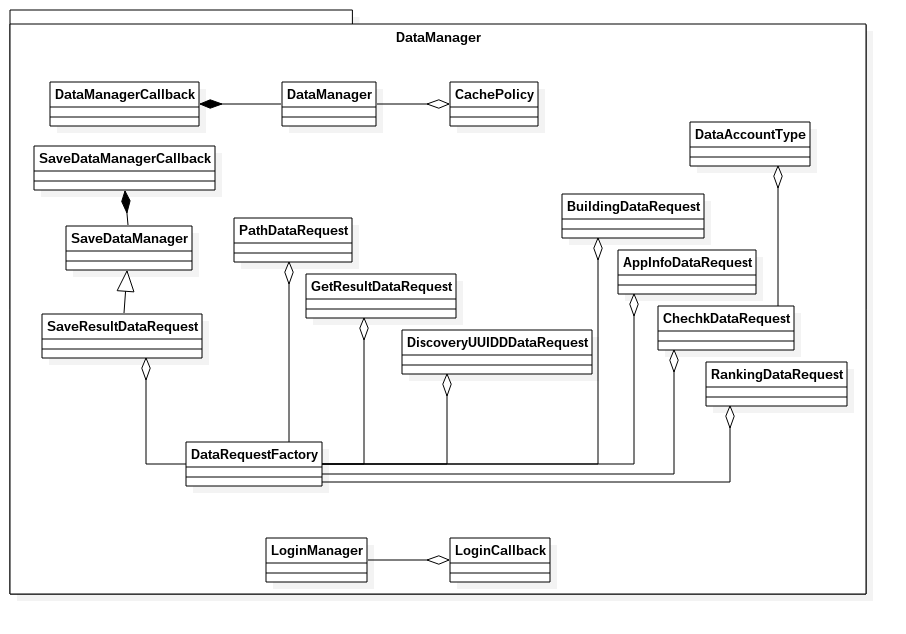
\includegraphics[scale=0.45]{img/package/png/client--datamanager--min.png}
	\caption{Schema sintetico package client::data::datamanager}
\end{figure}
\begin{figure}[h!]
	\centering
	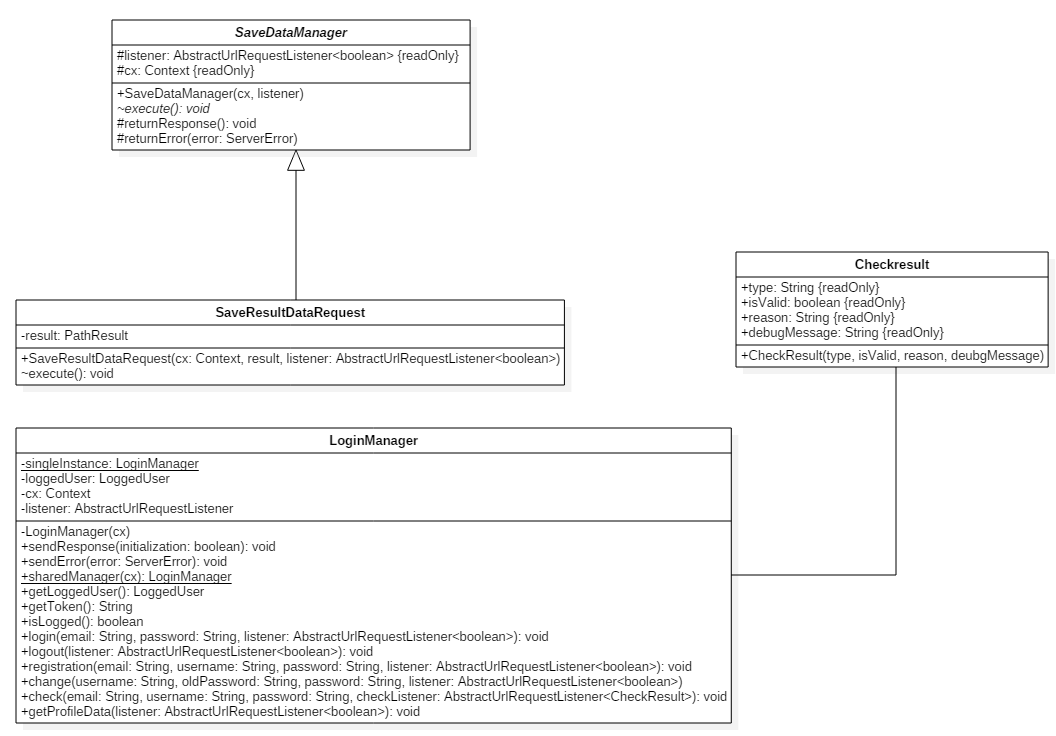
\includegraphics[scale=0.5]{img/package/png/client--datamanager1.png}
	\caption{Prima parte schema package client::data::datamanager}
\end{figure}
\begin{figure}[h!]
	\centering
	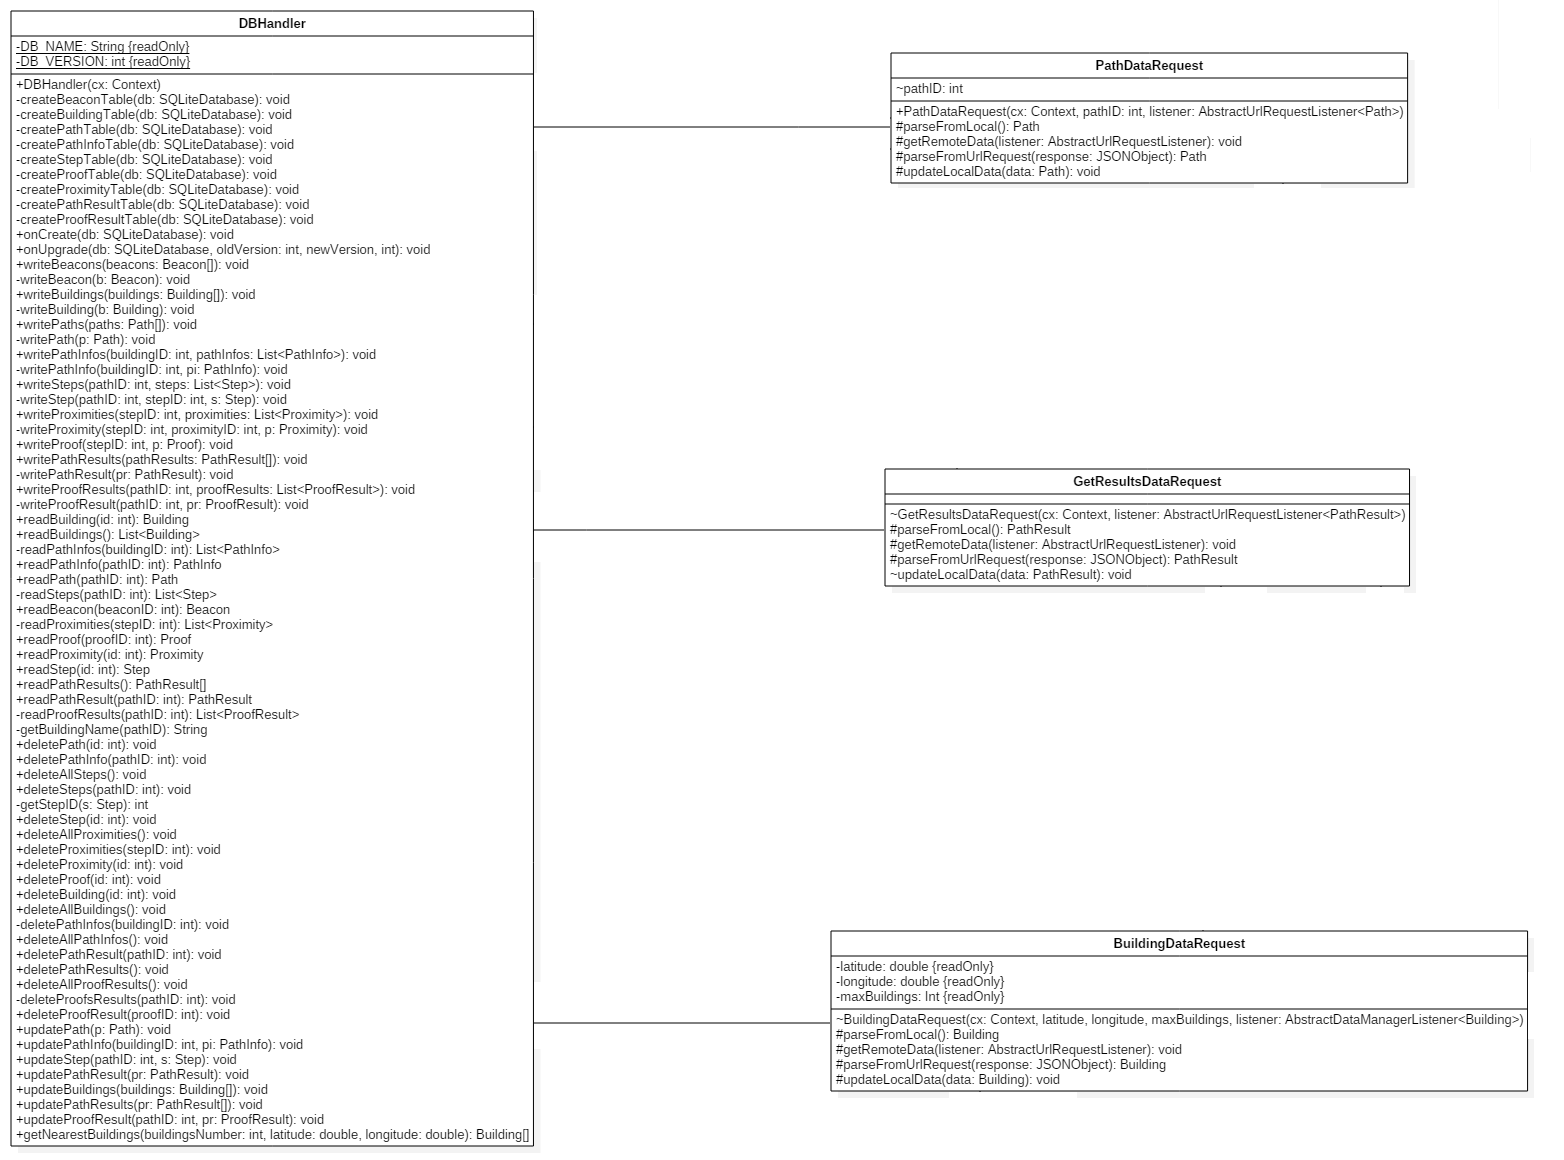
\includegraphics[scale=0.4]{img/package/png/client--datamanager2.png}
	\caption{Seconda parte schema package client::data::datamanager}
\end{figure}
\begin{figure}[h!]
	\centering
	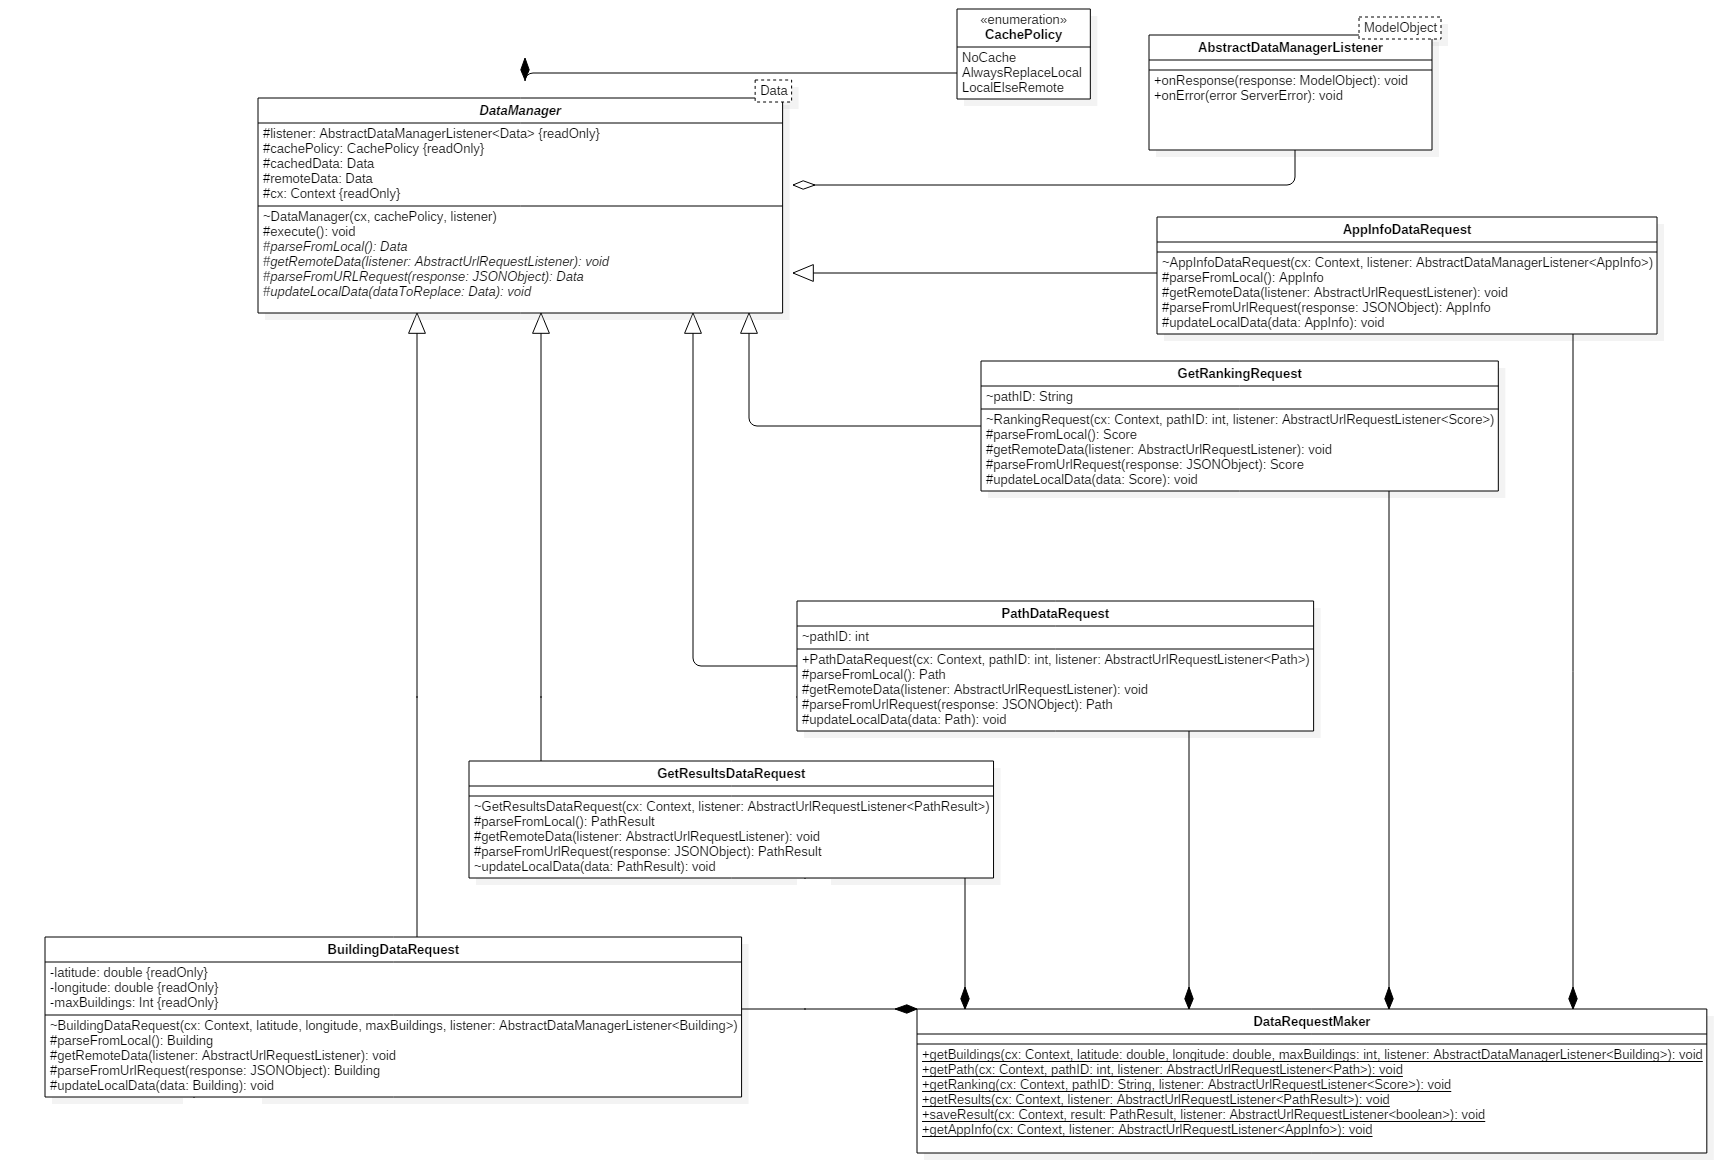
\includegraphics[scale=0.35]{img/package/png/client--datamanager3.png}
	\caption{Terza parte schema package client::data::datamanager}
\end{figure}
\compDescrizione{componente che gestisce i dati in locale}
\compPadre{data}
\begin{compClassi} \\
\begin{classe}{CLIPS::client::data::datamanager::\textit{SaveDataManager}}
\classeDescrizione{classe astratta per il salvataggio di dati nel server}
\classeUtilizzo{permette di effettuare il salvataggio dei dati nel server}
\begin{classeAttributi}
\classeAttributo{cx}{Context}{è una classe delle librerie base di Android che costituisce il cuore dell'applicazione, e quindi è necessaria per poter effettuare alcune operazioni, tra cui le richieste al server}
\classeAttributo{listener}{AbstractDataManagerListener<Boolean>}{il listener che verrà usato per informare l'applicazione se il salvataggio dei dati ha avuto successo o meno}
\end{classeAttributi}
\begin{classeMetodi}
\classeMetodo{execute}{}{void}{metodo astratto che effettua la richiesta al server necessaria, definita dall'implementazione concreta delle sottoclassi}
\classeMetodo{returnError}{error}{void}{chiama il metodo onError del listener}
\begin{classeMetodoArgomenti}
\classeMetodoArgomento{error}{ServerError}{oggetto che contiene le informazioni relative all'errore rilevato dall'applicazione durante il salvataggio dei dati del percorso svolto }
\end{classeMetodoArgomenti}
\classeMetodo{returnResponse}{}{void}{chiama il metodo onResponse del listener e ritorna sempre \texttt{true}, è un valore che serve solo per mantenere la consistenza della struttura del listener perché già chiamare il metodo indica che l'operazione è riuscita}
\end{classeMetodi}
\begin{classeRelazioni}
\classeRelazione{CLIPS::client::data::datamanager}{AbstractDataManagerListener}{interfaccia che definisce la struttura de listener astratto usato nel package datamanager}\classeRelazione{CLIPS::client::data::urlrequest}{ServerError}{classe che rappresenta l'errore che il client riceve quando la richiesta al server non ha successo}\end{classeRelazioni}\end{classe}
\begin{figure}[h!]
	\centering
	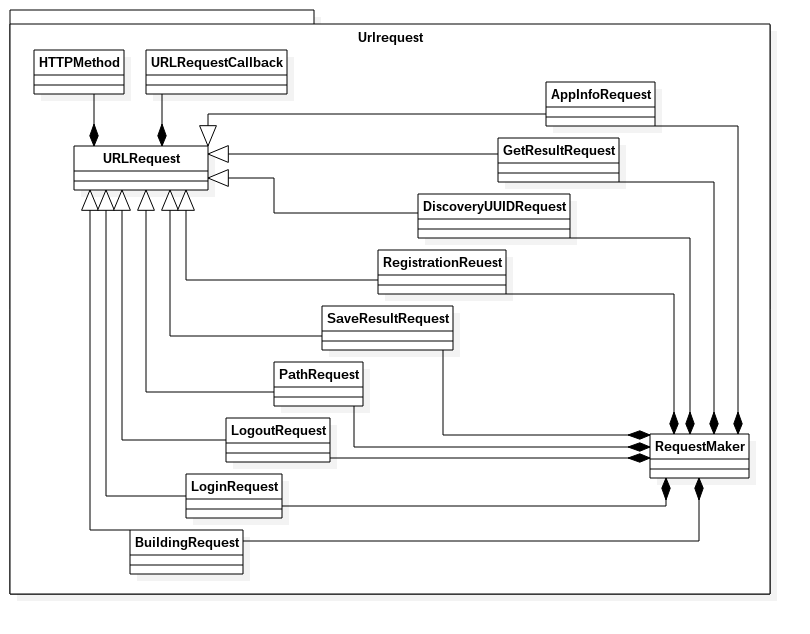
\includegraphics[scale=0.45]{img/package/png/client--urlrequest--min.png}
	\caption{Schema sintetico package client::data::urlrequest}
\end{figure}
\begin{figure}[h!]
	\centering
	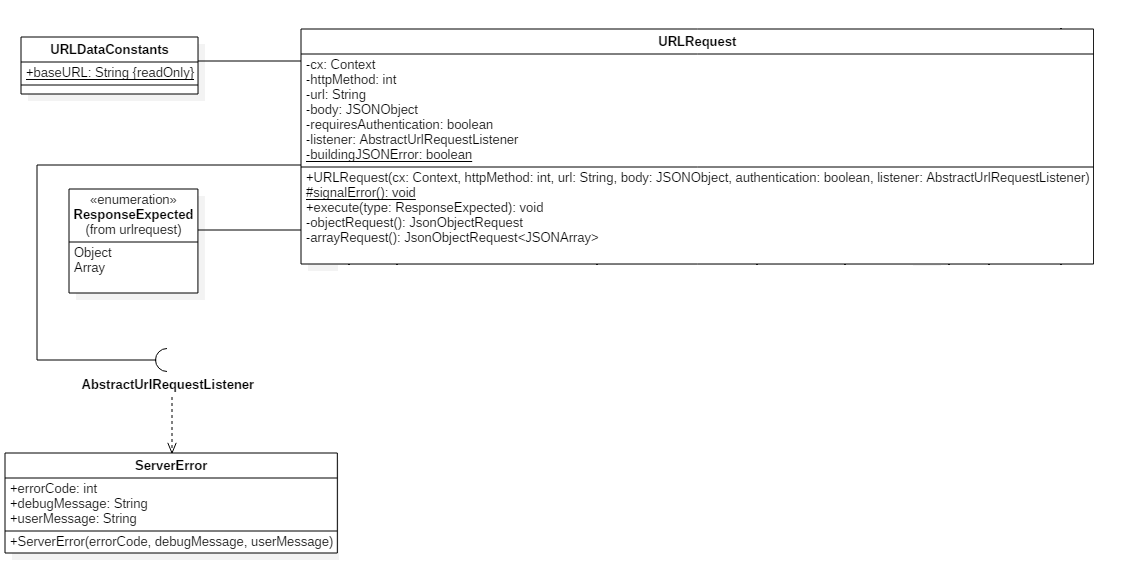
\includegraphics[scale=0.5]{img/package/png/client--urlrequest1.png}
	\caption{Prima parte schema package client::data::urlrequest}
\end{figure}
\begin{figure}[h!]
	\centering
	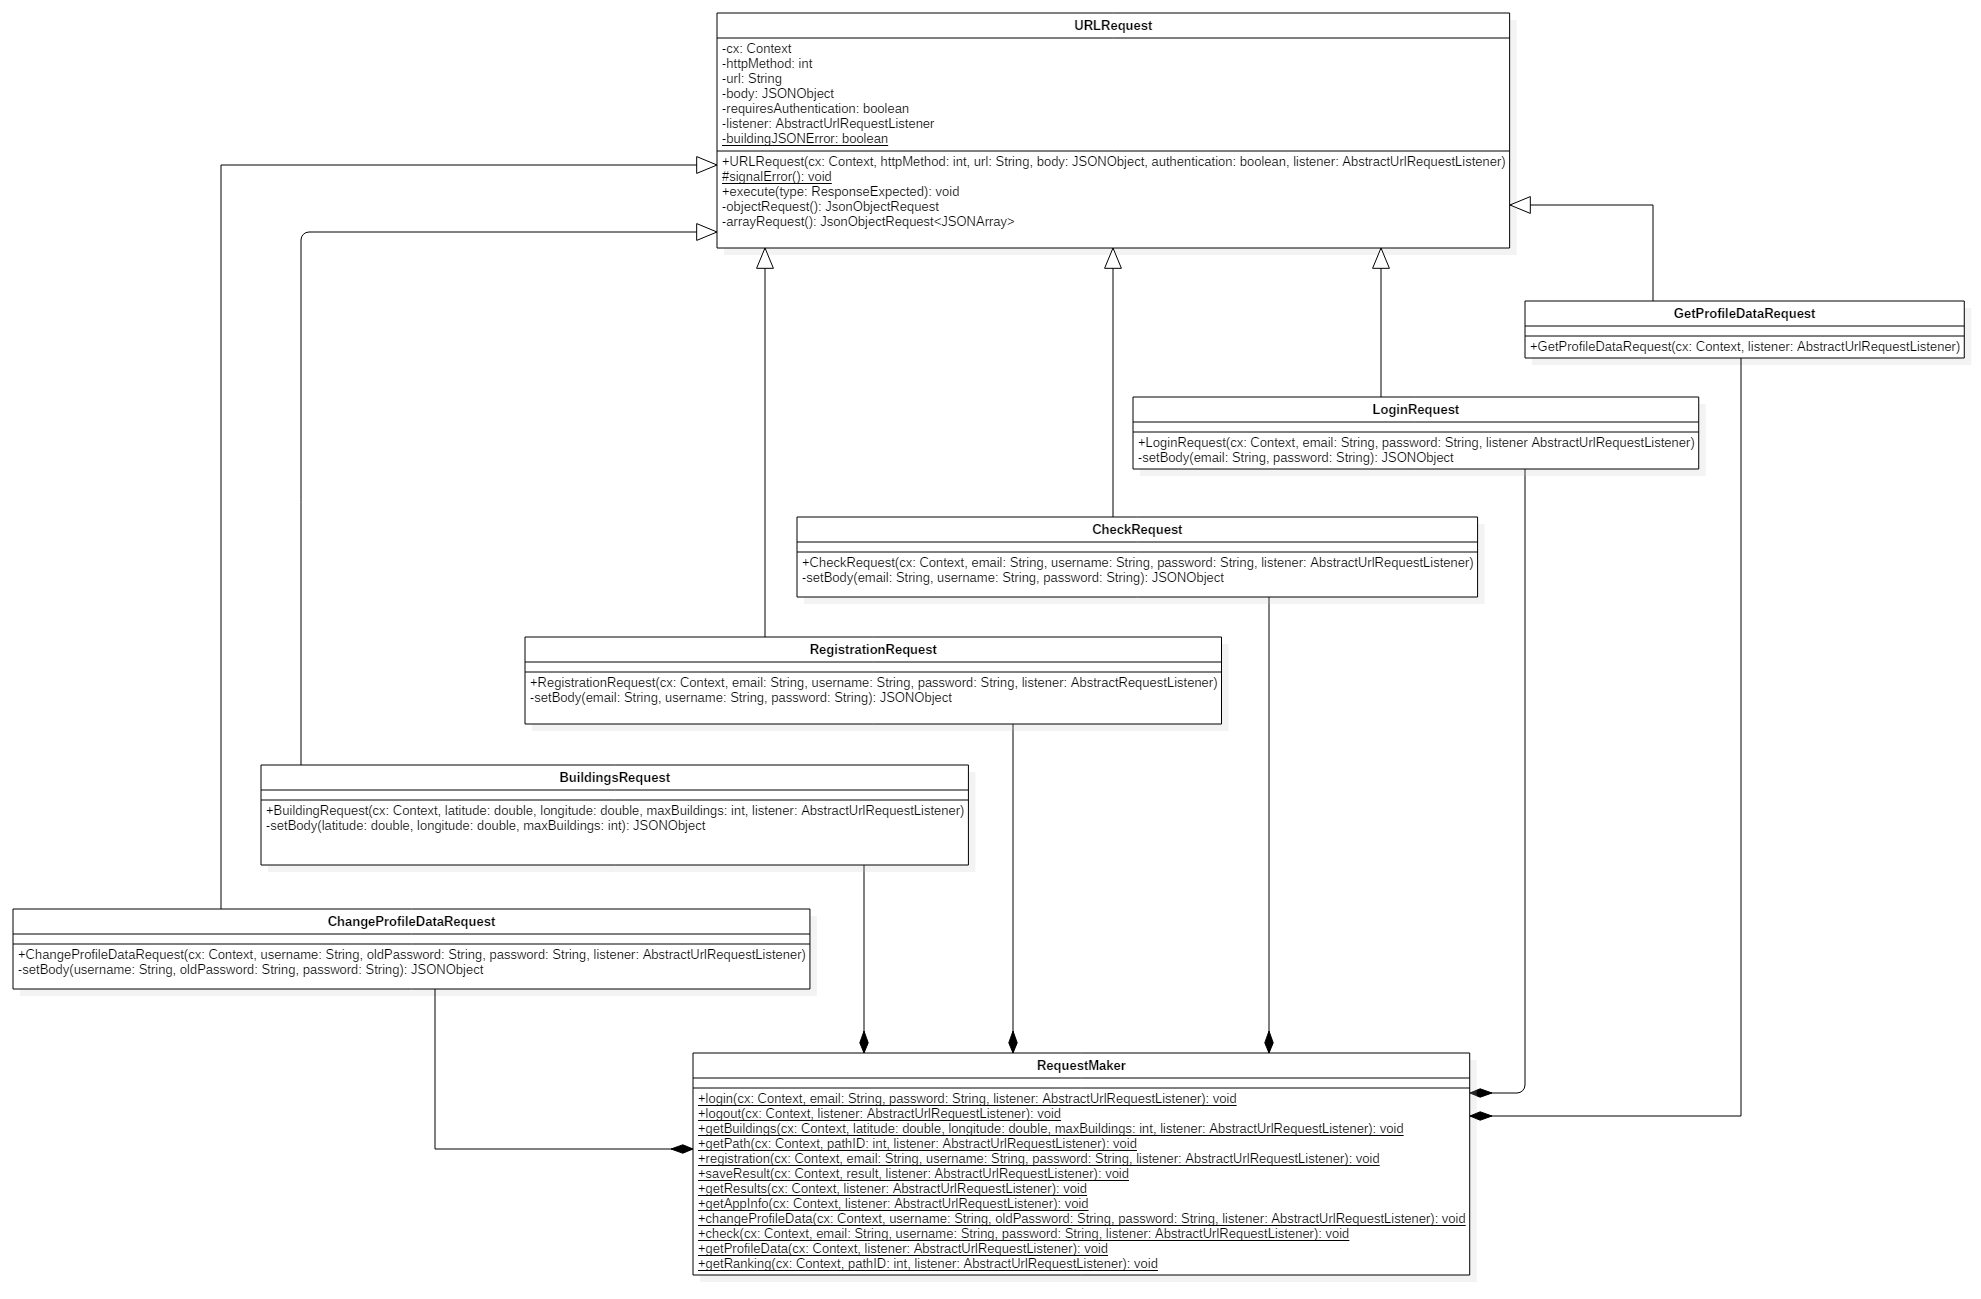
\includegraphics[scale=0.30]{img/package/png/client--urlrequest2.png}
	\caption{Seconda parte schema package client::data::urlrequest}
\end{figure}
\begin{figure}[h!]
	\centering
	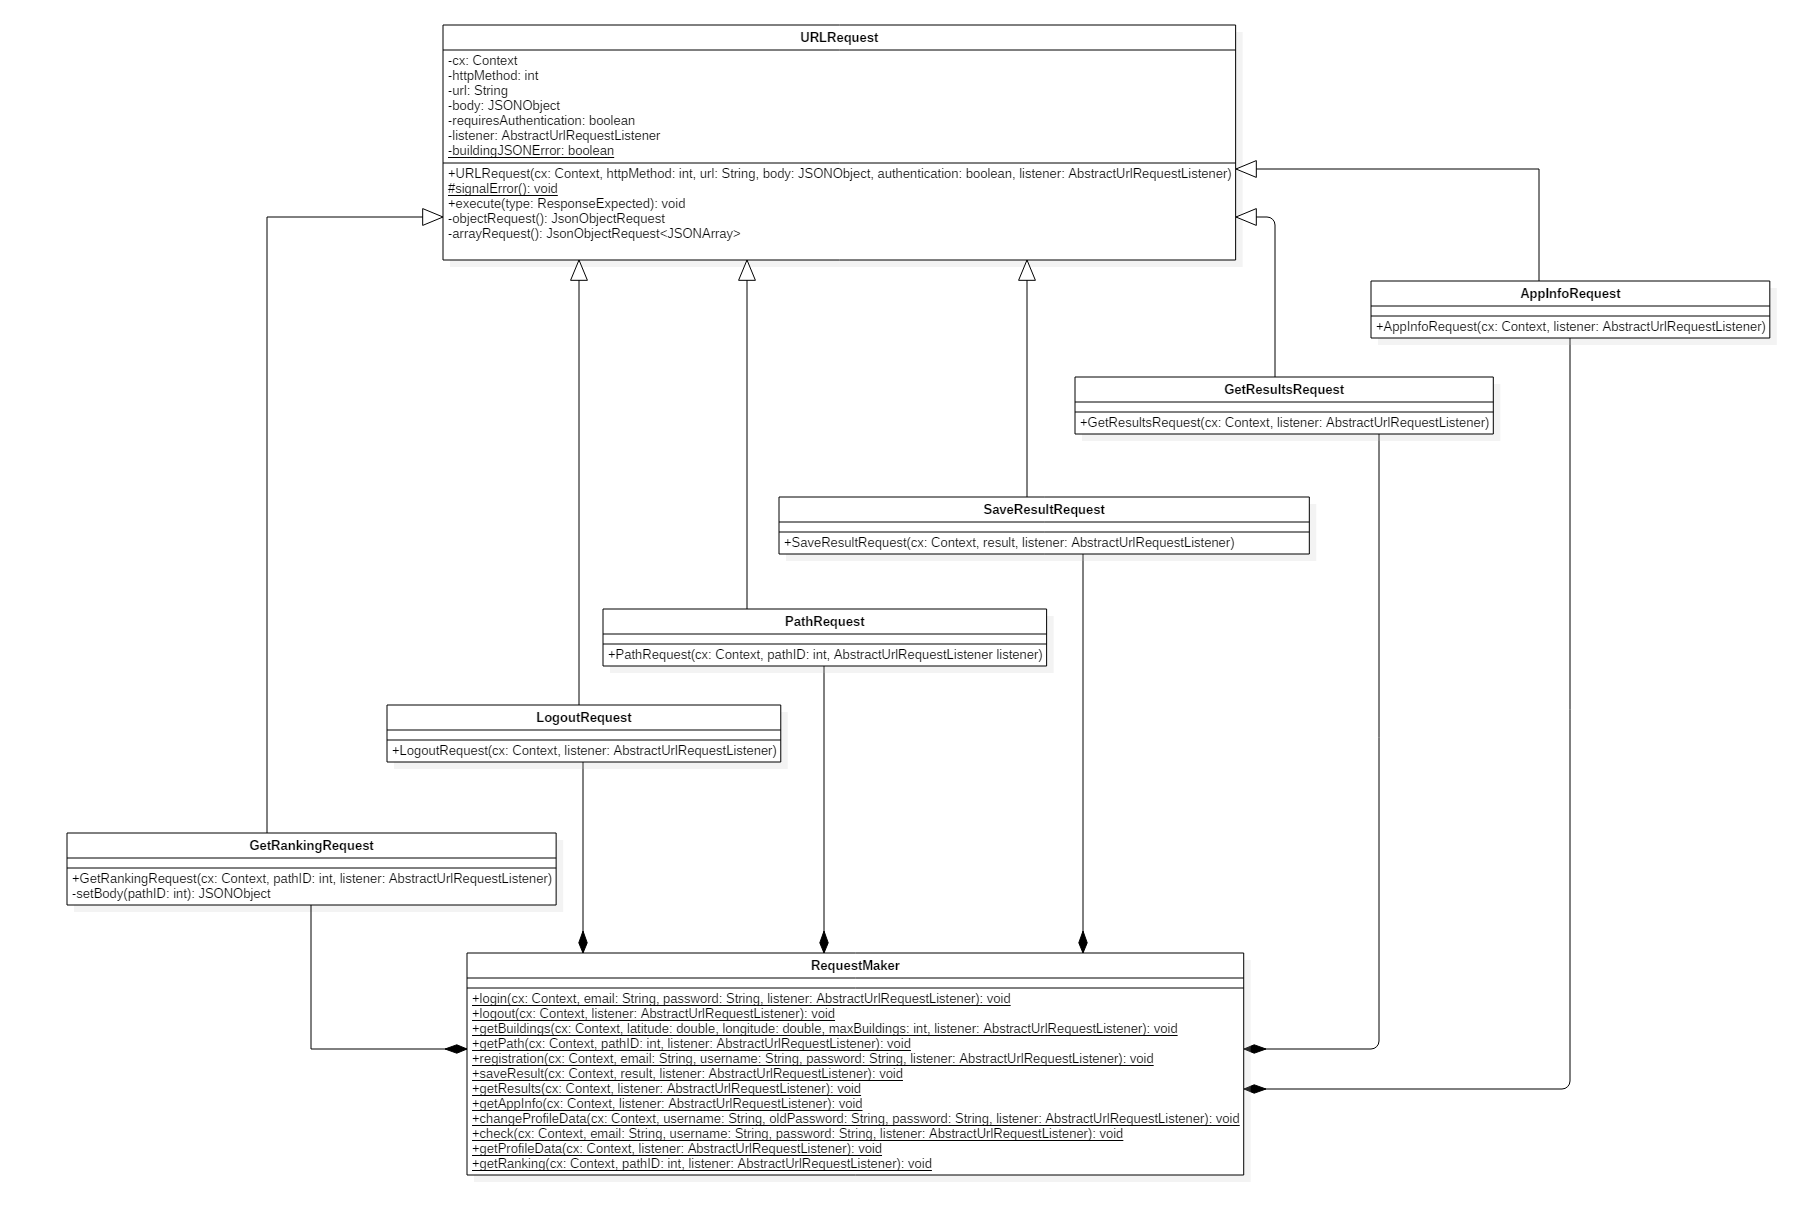
\includegraphics[scale=0.35]{img/package/png/client--urlrequest3.png}
	\caption{Terza parte schema package client::data::urlrequest}
\end{figure}

\begin{classe}{CLIPS::client::data::datamanager::AbstractDataManagerListener}
\classeDescrizione{interfaccia che definisce la struttura de listener astratto usato nel package datamanager}
\classeUtilizzo{permette alle classi che interagiscono con il datamanager di definire un proprio listener concreto da poter usare per ottenere le informazioni richieste}
\begin{classeMetodi}
\classeMetodo{onError}{error}{void}{metodo che viene invocato quando si ottiene un errore mentre si cerca di ricavare il dato richiesto}
\begin{classeMetodoArgomenti}
\classeMetodoArgomento{error}{ServerError}{l'errore ottenuto durante la ricerca del dato richiesto}
\end{classeMetodoArgomenti}
\classeMetodo{onResponse}{response}{void}{metodo che viene invocato quando si ottiene con successo il dato richiesto}
\begin{classeMetodoArgomenti}
\classeMetodoArgomento{response}{ModelObject}{è l'oggetto ricavato dal server o dal database locale}
\end{classeMetodoArgomenti}
\end{classeMetodi}
\begin{classeRelazioni}
\classeRelazione{CLIPS::client::data::urlrequest}{ServerError}{classe che rappresenta l'errore che il client riceve quando la richiesta al server non ha successo}\end{classeRelazioni}
\end{classe}\begin{classe}{CLIPS::client::data::datamanager::AppInfoDataRequest}
\classeDescrizione{classe concreta che gestisce le richieste dei dati sulle info dell'app}
\classeUtilizzo{permette di ottenere i dati sulle informazioni dell'app}
\begin{classeRelazioni}
\classeRelazione{CLIPS::client::data::datamanager}{AbstractDataManagerListener}{interfaccia che definisce la struttura de listener astratto usato nel package datamanager}\classeRelazione{CLIPS::client::data::urlrequest}{AbstractUrlRequestListener}{interfaccia che definisce la struttura del listener astratto usato nel package urlrequest}\classeRelazione{CLIPS::client::data::urlrequest}{AbstractUrlRequestListener}{interfaccia che definisce la struttura del listener astratto usato nel package urlrequest}\classeRelazione{CLIPS::client::data}{AppInfo}{classe per la rappresentazione delle informazioni dell'applicazione}\classeRelazione{CLIPS::client::data::urlrequest}{RequestMaker}{classe per la costruzione e l'invio di richieste al server, funziona come un'interfaccia dell'urlrequest per il resto dell'applicazione e quindi regola l'interazione con il package}\classeRelazione{CLIPS::client::data::urlrequest}{ServerError}{classe che rappresenta l'errore che il client riceve quando la richiesta al server non ha successo}\end{classeRelazioni}
\end{classe}\begin{classe}{CLIPS::client::data::datamanager::BuildingsDataRequest}
\classeDescrizione{classe concreta che gestisce le richieste dei dati sugli edifici}
\classeUtilizzo{permette di ottenere i dati sugli edifici}
\begin{classeAttributi}
\classeAttributo{latitude}{double}{la latitudine dell'utente}
\classeAttributo{longitude}{double}{la longitudine dell'utente}
\classeAttributo{maxBuildings}{int}{il numero massimo di edifici richiesti, serve per limitare la quantità di dati da ricevere dal server o da leggere dal database locale}
\end{classeAttributi}
\begin{classeRelazioni}
\classeRelazione{CLIPS::client::data::datamanager}{AbstractDataManagerListener}{interfaccia che definisce la struttura de listener astratto usato nel package datamanager}\classeRelazione{CLIPS::client::data::urlrequest}{AbstractUrlRequestListener}{interfaccia che definisce la struttura del listener astratto usato nel package urlrequest}\classeRelazione{CLIPS::client::data}{Building}{classe che rappresenta un edificio}\classeRelazione{CLIPS::server::urlrequesthandler}{DBHandler}{classe che si occupa di gestire il DB e di ritornare un oggetto configurato della libreria knex}\classeRelazione{CLIPS::client::data}{PathInfo}{classe che si occupa di salvare in locale le informazioni generali di un percorso}\classeRelazione{CLIPS::client::data::urlrequest}{RequestMaker}{classe per la costruzione e l'invio di richieste al server, funziona come un'interfaccia dell'urlrequest per il resto dell'applicazione e quindi regola l'interazione con il package}\classeRelazione{CLIPS::client::data::urlrequest}{ServerError}{classe che rappresenta l'errore che il client riceve quando la richiesta al server non ha successo}\end{classeRelazioni}
\end{classe}\begin{classe}{CLIPS::client::data::datamanager::CheckResult}
\classeDescrizione{classe che contiene il risultato del check per il dato specificato}
\classeUtilizzo{contiene tutte le informazioni sul dato controllato dal server, ovvero se è valido e il messaggio d'errore quando ne viene rilevato uno}
\begin{classeAttributi}
\classeAttributo{debugMessage}{string}{indica il motivo per cui il dato non è valido attraverso una spiegazione più tecnica, è destinato agli sviluppatori per aiutarli a trovare i bug nell'applicazione}
\classeAttributo{isValid}{boolean}{indica se il dato controllato ha un formato valido o no}
\classeAttributo{reason}{string}{indica il motivo per cui il dato non è valido}
\classeAttributo{type}{string}{il tipo di dato controllato, i possibili valori attesi sono \texttt{email}, \texttt{password} e \texttt{username}}
\end{classeAttributi}
\end{classe}\begin{classe}{CLIPS::client::data::datamanager::DataManager}
\classeDescrizione{classe astratta per la gestione della memorizzazione e del prelievo dei dati necessari per il funzionamento dell'applicazione}
\classeUtilizzo{permette di prelevare i dati dal server o in locale ed eventualmente di salvarli nel database locale}
\begin{classeAttributi}
\classeAttributo{cachedData}{Data}{oggetto generico in cui vengono memorizzati i dati letti dal database locale}
\classeAttributo{cachePolicy}{CachePolicy}{indica il comportamento dell'applicazione per la memorizzazione dei dati richiesti: \texttt{NoCache} indica che i dati vengono richiesti al server e mai salvati in locale; \texttt{AlwaysReplaceLocal} significa che i dati vengono richiesti al server, se vengono ricevuti allora i dati del database locale corrispondenti vengono sostituiti da quelli appena ottenuti, altrimenti vengono usati i dati salvati in locale; \texttt{LocalElseRemote} indica che vengono usati i dati del database locale, se non ci sono vengono richiesti al server}
\classeAttributo{cx}{Context}{è una classe delle librerie base di Android che costituisce il cuore dell'applicazione, e quindi è necessaria per poter effettuare alcune operazioni, tra cui le richieste al server}
\classeAttributo{listener}{AbstractDataManagerListener<Building[]>}{il listener che verrà usato per informare l'applicazione se l'operazione prevista ha avuto successo o meno}
\classeAttributo{remoteData}{Data}{oggetto generico in cui vengono memorizzati i dati ricevuti dal server}
\end{classeAttributi}
\begin{classeMetodi}
\classeMetodo{execute}{}{void}{metodo in cui vengono definite le operazioni da usare per i vari tipi di cachePolicy, per definire tali operazioni vengono usati i metodi astratti di DataManager}
\classeMetodo{getRemoteData}{listener}{void}{metodo astratto che effettua la richiesta al server per ottenere i dati richiesti}
\begin{classeMetodoArgomenti}
\classeMetodoArgomento{listener}{AbstractUrlRequestListener}{il listener che verrà usato per informare l'applicazione se la richiesta al server ha avuto successo o meno}
\end{classeMetodoArgomenti}
\classeMetodo{parseFromLocal}{}{Data}{metodo astratto dove vengono definite le operazioni per leggere i dati richiesti dal database locale}
\classeMetodo{parseFromUrlRequest}{response}{Data}{metodo astratto per estrarre i dati richiesti dal JSON ottenuto con la richiesta al server}
\begin{classeMetodoArgomenti}
\classeMetodoArgomento{response}{JSONObject}{l'oggetto JSON da cui estrarre i dati richiesti}
\end{classeMetodoArgomenti}
\classeMetodo{updateLocalData}{dataToReplace}{void}{metodo astratto che cancella i dati del database locale per sostituirli con quelli ricevuti dal server}
\begin{classeMetodoArgomenti}
\classeMetodoArgomento{dataToReplace}{Data}{i dati ottenuti dal server che devono rimpiazzare quelli salvati nel database locale}
\end{classeMetodoArgomenti}
\end{classeMetodi}
\begin{classeRelazioni}
\classeRelazione{CLIPS::client::data::datamanager}{AbstractDataManagerListener}{interfaccia che definisce la struttura de listener astratto usato nel package datamanager}\classeRelazione{CLIPS::client::data::urlrequest}{AbstractUrlRequestListener}{interfaccia che definisce la struttura del listener astratto usato nel package urlrequest}\classeRelazione{CLIPS::client::data::urlrequest}{ServerError}{classe che rappresenta l'errore che il client riceve quando la richiesta al server non ha successo}\end{classeRelazioni}
\end{classe}\begin{classe}{CLIPS::client::data::datamanager::DataRequestMaker}
\classeDescrizione{classe che effettua le operazioni di ricerca e salvataggio dei dati}
\classeUtilizzo{permette di effettuare operazioni di salvataggio dei dati nel server e di ricerca dei dati, richiedendoli al server o cercandoli in locale}
\begin{classeMetodi}
\classeMetodo{getAppInfo}{cx, listener}{void}{crea l'oggetto per ottenere le informazioni sull'applicazione dal server}
\begin{classeMetodoArgomenti}
\classeMetodoArgomento{cx}{Context}{è una classe delle librerie base di Android che costituisce il cuore dell'applicazione, e quindi è necessaria per poter effettuare alcune operazioni, tra cui le richieste al server}
\classeMetodoArgomento{listener}{AbstractDataManagerListener<AppInfo>}{il listener che verrà usato per informare l'applicazione se la ricerca dei dati ha avuto successo o meno}
\end{classeMetodoArgomenti}
\classeMetodo{getBuldings}{cx, latitude, listener, longitude, maxBuildings}{void}{crea l'oggetto per ottenere la lista degli edifici da visualizzare nell'applicazione, prima cercandoli nel server e poi, in caso ci siano problemi, nel database locale}
\begin{classeMetodoArgomenti}
\classeMetodoArgomento{cx}{Context}{è una classe delle librerie base di Android che costituisce il cuore dell'applicazione, e quindi è necessaria per poter effettuare alcune operazioni, tra cui le richieste al server}
\classeMetodoArgomento{latitude}{double}{la latitudine attuale dell'utente}
\classeMetodoArgomento{listener}{AbstractDataManagerListener<Building[]>}{il listener che verrà usato per informare l'applicazione se la ricerca dei dati ha avuto successo o meno}
\classeMetodoArgomento{longitude}{double}{la longitudine attuale dell'utente}
\classeMetodoArgomento{maxBuildings}{int}{il numero massimo di edifici richiesti, serve per limitare l'elenco ottenuto}
\end{classeMetodoArgomenti}
\classeMetodo{getPath}{cx, listener, pathID}{void}{crea l'oggetto per ottenere i dati del percorso selezionato, prima cercandoli nel server e poi, in caso ci siano problemi, nel database locale}
\begin{classeMetodoArgomenti}
\classeMetodoArgomento{cx}{Context}{è una classe delle librerie base di Android che costituisce il cuore dell'applicazione, e quindi è necessaria per poter effettuare alcune operazioni, tra cui le richieste al server}
\classeMetodoArgomento{listener}{AbstractDataManagerListener<Path>}{il listener che verrà usato per informare l'applicazione se la ricerca dei dati ha avuto successo o meno}
\classeMetodoArgomento{pathID}{int}{l'ID del percorso selezionato}
\end{classeMetodoArgomenti}
\classeMetodo{getRanking}{cx, listener, pathID}{void}{crea l'oggetto per ottenere la classifica del percorso selezionato dal server}
\begin{classeMetodoArgomenti}
\classeMetodoArgomento{cx}{Context}{è una classe delle librerie base di Android che costituisce il cuore dell'applicazione, e quindi è necessaria per poter effettuare alcune operazioni, tra cui le richieste al server}
\classeMetodoArgomento{listener}{AbstractDataManagerListener<PlayerRanking[]>}{il listener che verrà usato per informare l'applicazione se la ricerca dei dati ha avuto successo o meno}
\classeMetodoArgomento{pathID}{int}{l'ID del percorso selezionato}
\end{classeMetodoArgomenti}
\classeMetodo{getResults}{cx, listener}{void}{crea l'oggetto per ottenere la lista di tutti i risultati dell'utente, prima cercandoli nel server e poi, in caso ci siano problemi, nel database locale}
\begin{classeMetodoArgomenti}
\classeMetodoArgomento{cx}{Context}{crea l'oggetto per ottenere la lista degli edifici da visualizzare nell'applicazione, prima cercandoli nel server e poi, in caso ci siano problemi, nel database locale}
\classeMetodoArgomento{listener}{AbstractDataManagerListener<PathResult[]>}{il listener che verrà usato per informare l'applicazione se la ricerca dei dati ha avuto successo o meno}
\end{classeMetodoArgomenti}
\classeMetodo{saveResult}{cx, listener, pathResult}{void}{crea l'oggetto per salvare nel server il risultato appena ottenuto}
\begin{classeMetodoArgomenti}
\classeMetodoArgomento{cx}{Context}{è una classe delle librerie base di Android che costituisce il cuore dell'applicazione, e quindi è necessaria per poter effettuare alcune operazioni, tra cui le richieste al server}
\classeMetodoArgomento{listener}{AbstractDataManagerListener<Boolean>}{il listener che verrà usato per informare l'applicazione se la ricerca dei dati ha avuto successo o meno}
\classeMetodoArgomento{pathResult}{PathResult}{contiene il risultato del percorso appena svolto dall'utente}
\end{classeMetodoArgomenti}
\end{classeMetodi}
\begin{classeRelazioni}
\classeRelazione{CLIPS::client::data::datamanager}{AbstractDataManagerListener}{interfaccia che definisce la struttura de listener astratto usato nel package datamanager}\classeRelazione{CLIPS::client::data}{AppInfo}{classe per la rappresentazione delle informazioni dell'applicazione}\classeRelazione{CLIPS::client::data::datamanager}{AppInfoDataRequest}{classe concreta che gestisce le richieste dei dati sulle info dell'app}\classeRelazione{CLIPS::client::data}{Building}{classe che rappresenta un edificio}\classeRelazione{CLIPS::client::data::datamanager}{BuildingsDataRequest}{classe concreta che gestisce le richieste dei dati sugli edifici}\classeRelazione{CLIPS::client::data::datamanager}{GetRankingDataRequest}{classe concreta che gestisce le richieste dei dati della classifica}\classeRelazione{CLIPS::client::data::datamanager}{GetResultsDataRequest}{classe concreta che gestisce le richieste dei dati dei risultati}\classeRelazione{CLIPS::client::data}{Path}{classe che si occupa di salvare in locale i dati riguardanti un percorso}\classeRelazione{CLIPS::client::data::datamanager}{PathDataRequest}{classe concreta che gestisce le richieste dei dati sui percorsi}\classeRelazione{CLIPS::client::data}{PathResult}{classe che rappresenta i risultati di un percorso}\classeRelazione{CLIPS::client::data::datamanager}{SaveResultDataRequest}{classe concreta che effettua le richieste per salvare il risultato del percorso appena concluso}\classeRelazione{CLIPS::client::data}{Score}{classe che rappresenta il risultato nella classifica dell'utente}\end{classeRelazioni}
\end{classe}\begin{classe}{CLIPS::client::data::datamanager::DBHandler}
\classeDescrizione{classe che si occupa dell'interazione con il database locale}
\classeUtilizzo{utilizzando questa classe è possibile interagire con il database locale per ottenere e salvare i dati desiderati}
\begin{classeAttributi}
\classeAttributo{DB\_NAME}{string}{costante statica contenente il nome del database locale}
\classeAttributo{DB\_VERSION}{int}{costante statica contenente la versione del database locale}
\end{classeAttributi}
\begin{classeMetodi}
\classeMetodo{createBeaconTable}{db}{void}{metodo per la creazione della tabella Beacon all'interno del database locale}
\begin{classeMetodoArgomenti}
\classeMetodoArgomento{db}{SQLiteDatabase}{oggetto necessario per l'interazione con il database locale}
\end{classeMetodoArgomenti}
\classeMetodo{createBuildingTable}{db}{void}{metodo per la creazione della tabella Building all'interno del database locale}
\begin{classeMetodoArgomenti}
\classeMetodoArgomento{db}{SQLiteDatabase}{oggetto necessario per l'interazione con il database locale}
\end{classeMetodoArgomenti}
\classeMetodo{createPathInfoTable}{db}{void}{metodo per la creazione della tabella PathInfo all'interno del database locale}
\begin{classeMetodoArgomenti}
\classeMetodoArgomento{db}{SQLiteDatabase}{oggetto necessario per l'interazione con il database locale}
\end{classeMetodoArgomenti}
\classeMetodo{createPathResultTable}{db}{void}{metodo per la creazione della tabella PathResult all'interno del database locale}
\begin{classeMetodoArgomenti}
\classeMetodoArgomento{db}{SQLiteDatabase}{oggetto necessario per l'interazione con il database locale}
\end{classeMetodoArgomenti}
\classeMetodo{createPathTable}{db}{void}{metodo per la creazione della tabella Path all'interno del database locale}
\begin{classeMetodoArgomenti}
\classeMetodoArgomento{db}{SQLiteDatabase}{oggetto necessario per l'interazione con il database locale}
\end{classeMetodoArgomenti}
\classeMetodo{createProofResultTable}{db}{void}{metodo per la creazione della tabella ProofResult all'interno del database locale}
\begin{classeMetodoArgomenti}
\classeMetodoArgomento{db}{SQLiteDatabase}{oggetto necessario per l'interazione con il database locale}
\end{classeMetodoArgomenti}
\classeMetodo{createProofTable}{}{void}{metodo per la creazione della tabella Proof all'interno del database locale}
\classeMetodo{createProximityTable}{db}{void}{metodo per la creazione della tabella Proximity all'interno del database locale}
\begin{classeMetodoArgomenti}
\classeMetodoArgomento{db}{SQLiteDatabase}{oggetto necessario per l'interazione con il database locale}
\end{classeMetodoArgomenti}
\classeMetodo{createStepTable}{db}{void}{metodo per la creazione della tabella Step all'interno del database locale}
\begin{classeMetodoArgomenti}
\classeMetodoArgomento{db}{SQLiteDatabase}{oggetto necessario per l'interazione con il database locale}
\end{classeMetodoArgomenti}
\classeMetodo{deleteAllBuildings}{}{void}{metodo per l'eliminazione di tutti gli oggetti Building dal database locale}
\classeMetodo{deleteAllPathInfos}{}{void}{metodo per l'eliminazione di tutti gli oggetti PathInfo dal database locale}
\classeMetodo{deleteAllProofResults}{}{void}{metodo per l'eliminazione di tutti gli oggetti ProofResult dal database locale}
\classeMetodo{deleteAllSteps}{}{void}{metodo per l'eliminazione di tutti gli oggetti Step salvati nel database locale}
\classeMetodo{deleteBuilding}{id}{void}{metodo per l'eliminazione di un singolo oggetto Building dal database locale}
\begin{classeMetodoArgomenti}
\classeMetodoArgomento{id}{int}{id dell'oggetto Building da eliminare}
\end{classeMetodoArgomenti}
\classeMetodo{deletePath}{id}{void}{metodo per l'eliminazione di un oggetto Path dal database locale}
\begin{classeMetodoArgomenti}
\classeMetodoArgomento{id}{int}{id dell'oggetto Path da eliminare}
\end{classeMetodoArgomenti}
\classeMetodo{deletePathInfo}{pathID}{void}{metodo per l'eliminazione dell'oggetto PathInfo relativo ad un oggetto Path dal database locale}
\begin{classeMetodoArgomenti}
\classeMetodoArgomento{pathID}{int}{id dell'oggetto Path da cui ricavare l'oggetto PathInfo da eliminare}
\end{classeMetodoArgomenti}
\classeMetodo{deletePathInfos}{buildingID}{void}{metodo per l'eliminazione di tutti gli oggetti PathInfo relativi ad un oggetto Building dal database locale}
\begin{classeMetodoArgomenti}
\classeMetodoArgomento{buildingID}{int}{id dell'oggetto Building da cui ricavare gli oggetti PathInfo da eliminare}
\end{classeMetodoArgomenti}
\classeMetodo{deletePathResult}{pathID}{void}{metodo per l'eliminazione dell'oggetto PathResult relativo ad un oggetto Path}
\begin{classeMetodoArgomenti}
\classeMetodoArgomento{pathID}{int}{id dell'oggetto Path da cui ricavare l'oggetto PathResult da eliminare}
\end{classeMetodoArgomenti}
\classeMetodo{deletePathResults}{}{void}{metodo per l'eliminazione di tutti gli oggetti PathResult dal database locale}
\classeMetodo{deleteProof}{id}{void}{metodo per l'eliminazione di un singolo oggetto Proof}
\begin{classeMetodoArgomenti}
\classeMetodoArgomento{id}{int}{id dell'oggetto Proof da eliminare}
\end{classeMetodoArgomenti}
\classeMetodo{deleteProofResult}{proofID}{void}{metodo per l'eliminazione di un oggetto ProofResult relativo ad un oggetto Proof}
\begin{classeMetodoArgomenti}
\classeMetodoArgomento{proofID}{int}{id dell'oggetto Proof da cui ricavare l'oggetto ProofResult da eliminare}
\end{classeMetodoArgomenti}
\classeMetodo{deleteProofResults}{pathID}{void}{metodo per l'eliminazione degli oggetti ProofResult relativi ad un oggetto PathResult}
\begin{classeMetodoArgomenti}
\classeMetodoArgomento{pathID}{int}{id dell'oggetto PathResult da cui ricavare gli oggetti ProofResult da eliminare}
\end{classeMetodoArgomenti}
\classeMetodo{deleteProximities}{stepID}{void}{metodo per l'eliminazione di tutti gli oggetti Proximity dal database locale}
\begin{classeMetodoArgomenti}
\classeMetodoArgomento{stepID}{int}{id dell'oggetto Step da cui ricavare gli oggetti Proximity da eliminare}
\end{classeMetodoArgomenti}
\classeMetodo{deleteProximity}{id}{void}{metodo per l'eliminazione di un singolo oggetto Proximity}
\begin{classeMetodoArgomenti}
\classeMetodoArgomento{id}{int}{id dell'oggetto Proximity da eliminare}
\end{classeMetodoArgomenti}
\classeMetodo{deleteStep}{id}{void}{metodo per l'eliminazione di un oggetto Step dal database locale}
\begin{classeMetodoArgomenti}
\classeMetodoArgomento{id}{int}{id dell'oggetto Step da eliminare}
\end{classeMetodoArgomenti}
\classeMetodo{deleteSteps}{pathID}{void}{metodo per l'eliminazione di tutti gli oggetti Step relativi ad un oggetto Path dal database locale}
\begin{classeMetodoArgomenti}
\classeMetodoArgomento{pathID}{int}{id dell'oggetto Path da cui ricavare gli oggetti Step da eliminare}
\end{classeMetodoArgomenti}
\classeMetodo{getBuildingName}{pathID}{string}{metodo per ricavare il nome dell'edificio a cui è associato un oggetto Path conosciuto}
\begin{classeMetodoArgomenti}
\classeMetodoArgomento{pathID}{int}{id dell'oggetto Path da cui ricavare il nome dell'edificio a cui l'oggetto è associato}
\end{classeMetodoArgomenti}
\classeMetodo{getNearestBuildings}{buildingNumber, latitude, longitude}{Building[]}{metodo per ottenere un array contenente i buildingNumber oggetti Building più vicini rispetto alle variabili latitude e longitude fornite}
\begin{classeMetodoArgomenti}
\classeMetodoArgomento{buildingNumber}{int}{numero degli oggetti Building più vicini all'utente rispetto alle sue coordinate}
\classeMetodoArgomento{latitude}{int}{valore della latitudine a cui si trova l'utente}
\classeMetodoArgomento{longitude}{int}{valore della longitudine a cui si trova l'utente}
\end{classeMetodoArgomenti}
\classeMetodo{getStepID}{s}{int}{metodo per ricavare l'id di un oggetto Step conosciuto e salvato nel database locale}
\begin{classeMetodoArgomenti}
\classeMetodoArgomento{s}{Step}{oggetto Step da cercare nel database locale per ricavarne l'id}
\end{classeMetodoArgomenti}
\classeMetodo{onCreate}{}{void}{metodo chiamato quando viene creato il database locale che a sua volta chiama tutti i metodi necessari per creare le tabelle del database}
\classeMetodo{readBeacon}{beaconID}{Beacon}{metodo per la lettura di un singolo oggetto Beacon dal database locale}
\begin{classeMetodoArgomenti}
\classeMetodoArgomento{beaconID}{int}{id dell'oggetto Beacon di cui si vogliono ottenere i dati}
\end{classeMetodoArgomenti}
\classeMetodo{readBuilding}{id}{Building}{metodo per la lettura di un singolo oggetto Building dal database locale}
\begin{classeMetodoArgomenti}
\classeMetodoArgomento{id}{int}{id dell'oggetto Building di cui si vogliono ottenere i dati}
\end{classeMetodoArgomenti}
\classeMetodo{readBuildings}{}{List<Building>}{metodo per la lettura di tutti gli oggetti Building presenti nel database locale}
\classeMetodo{readPath}{pathID}{Path}{metodo per la lettura di un oggetto Path dal database locale}
\begin{classeMetodoArgomenti}
\classeMetodoArgomento{pathID}{int}{id dell'oggetto Path di cui si vogliono ottenere i dati}
\end{classeMetodoArgomenti}
\classeMetodo{readPathInfo}{pathID}{PathInfo}{metodo per la lettura dell'oggetto PathInfo relativo ad un oggetto Path}
\begin{classeMetodoArgomenti}
\classeMetodoArgomento{pathID}{int}{id dell'oggetto Path da cui ricavare l'oggetto PathInfo}
\end{classeMetodoArgomenti}
\classeMetodo{readPathInfos}{buildingID}{List<PathInfo>}{metodo per la lettura di tutti gli oggetti PathInfo relativi ad un oggetto Building presenti nel database locale}
\begin{classeMetodoArgomenti}
\classeMetodoArgomento{buildingID}{int}{id dell'oggetto Building da cui ricavare la lista degli oggetti PathInfo}
\end{classeMetodoArgomenti}
\classeMetodo{readPathResult}{pathID}{PathResult}{metodo per la lettura dell'oggetto PathResult relativo ad un oggetto Path}
\begin{classeMetodoArgomenti}
\classeMetodoArgomento{pathID}{int}{id dell'oggetto Path da cui ricavare l'oggetto PathResult}
\end{classeMetodoArgomenti}
\classeMetodo{readPathResults}{}{PathResult[]}{metodo per la lettura di tutti gli oggetti PathResult dell'utente presenti nel database locale}
\classeMetodo{readProof}{proofID}{Proof}{metodo per la lettura di un singolo oggetto Proof dal database locale}
\begin{classeMetodoArgomenti}
\classeMetodoArgomento{proofID}{int}{id dell'oggetto Proof di cui si vogliono ottenere i dati}
\end{classeMetodoArgomenti}
\classeMetodo{readProofResults}{pathID}{List<ProofResult>}{metodo per la lettura di tutti gli oggetti ProofResult relativi ad un oggetto Path presenti nel database locale}
\begin{classeMetodoArgomenti}
\classeMetodoArgomento{pathID}{int}{id dell'oggetto Path da cui ricavare la lista degli oggetti ProofResult}
\end{classeMetodoArgomenti}
\classeMetodo{readProximities}{stepID}{List<Proximity>}{metodo per la lettura di tutti gli oggetti Proximity relativi ad un oggetto Step presenti nel database locale}
\begin{classeMetodoArgomenti}
\classeMetodoArgomento{stepID}{int}{id dell'oggetto Step da cui ricavare la lista di oggetti Step}
\end{classeMetodoArgomenti}
\classeMetodo{readProximity}{id}{Proximity}{metodo per la lettura di un singolo oggetto Proximity dal database locale}
\begin{classeMetodoArgomenti}
\classeMetodoArgomento{id}{int}{id dell'oggetto Proximity di cui si vogliono ottenere i dati}
\end{classeMetodoArgomenti}
\classeMetodo{readStep}{id}{Step}{metodo per la lettura di un singolo oggetto Step dal database locale}
\begin{classeMetodoArgomenti}
\classeMetodoArgomento{id}{int}{id dell'oggetto Step di cui si vogliono ottenere i dati}
\end{classeMetodoArgomenti}
\classeMetodo{readSteps}{pathID}{List<Step>}{metodo per la lettura di tutti gli oggetti Step relativi ad un oggetto Path presenti nel database locale}
\begin{classeMetodoArgomenti}
\classeMetodoArgomento{pathID}{int}{id dell'oggetto Path da cui ricavare la lista degli oggetti Step}
\end{classeMetodoArgomenti}
\classeMetodo{updateBuildings}{buildings}{void}{metodo per aggiornare gli oggetti Building salvati nel database locale eliminando tutti gli oggetti Building presenti ed inserendone di nuovi}
\begin{classeMetodoArgomenti}
\classeMetodoArgomento{buildings}{Building[]}{array contenente gli oggetti Building da inserire}
\end{classeMetodoArgomenti}
\classeMetodo{updatePath}{p}{void}{metodo per l'aggiornamento di un oggetto Path nel database locale}
\begin{classeMetodoArgomenti}
\classeMetodoArgomento{p}{Path}{oggetto da aggiornare nel database locale}
\end{classeMetodoArgomenti}
\classeMetodo{updatePathInfo}{buildingID, pi}{void}{metodo per l'aggiornamento di un oggetto PathInfo nel database locale}
\begin{classeMetodoArgomenti}
\classeMetodoArgomento{buildingID}{int}{id dell'oggetto Building a cui l'oggetto PathInfo da aggiornare è associato}
\classeMetodoArgomento{pi}{PathInfo}{oggetto PathInfo da aggiornare}
\end{classeMetodoArgomenti}
\classeMetodo{updatePathResult}{pr}{void}{metodo per l'aggiornamento di un oggetto PathResult nel database locale}
\begin{classeMetodoArgomenti}
\classeMetodoArgomento{pr}{PathResult}{oggetto PathResult da aggiornare}
\end{classeMetodoArgomenti}
\classeMetodo{updatePathResults}{pathResults}{void}{metodo per aggiornare gli oggetti PathResult salvati nel database locale eliminando tutti gli oggetti PathResult presenti ed inserendone di nuovi}
\begin{classeMetodoArgomenti}
\classeMetodoArgomento{pathResults}{PathResult[]}{array contenente gli oggetti PathResult da inserire}
\end{classeMetodoArgomenti}
\classeMetodo{updateProofResult}{pathID, pr}{void}{metodo per l'aggiornamento di un oggetto ProofResult nel database locale}
\begin{classeMetodoArgomenti}
\classeMetodoArgomento{pathID}{int}{id dell'oggetto PathResult a cui l'oggetto ProofResult è associato}
\classeMetodoArgomento{pr}{ProofResult}{oggetto ProofResult da aggiornare}
\end{classeMetodoArgomenti}
\classeMetodo{updateStep}{pathID, s}{void}{metodo per l'aggiornamento di un oggetto Step nel database locale}
\begin{classeMetodoArgomenti}
\classeMetodoArgomento{pathID}{int}{id dell'oggetto Path a cui l'oggetto Step da aggiornare è associato}
\classeMetodoArgomento{s}{Step}{oggetto Step da aggiornare}
\end{classeMetodoArgomenti}
\classeMetodo{writeBeacon}{b}{void}{metodo per l'inserimento di un singolo oggetto Beacon all'interno del database locale}
\begin{classeMetodoArgomenti}
\classeMetodoArgomento{b}{Beacon}{oggetto Beacon da salvare nel database locale}
\end{classeMetodoArgomenti}
\classeMetodo{writeBeacons}{beacons}{void}{metodo per l'inserimento multiplo di oggetti Beacon nel database locale}
\begin{classeMetodoArgomenti}
\classeMetodoArgomento{beacons}{Beacon[]}{array contenente gli oggetti di tipo Beacon da inserire nel database locale}
\end{classeMetodoArgomenti}
\classeMetodo{writeBuilding}{b, id}{void}{metodo per l'inserimento di un singolo oggetto Building all'interno del database locale}
\begin{classeMetodoArgomenti}
\classeMetodoArgomento{b}{Building}{oggetto Beacon da salvare nel database locale}
\classeMetodoArgomento{id}{int}{id dell'oggetto da inserire nel database}
\end{classeMetodoArgomenti}
\classeMetodo{writeBuildings}{buildings}{void}{metodo per l'inserimento multiplo di oggetti Building nel database locale}
\begin{classeMetodoArgomenti}
\classeMetodoArgomento{buildings}{Building[]}{array contenente gli oggetti di tipo Building da inserire nel database locale}
\end{classeMetodoArgomenti}
\classeMetodo{writePath}{p}{void}{metodo per l'inserimento di un singolo oggetto Path all'interno del database locale}
\begin{classeMetodoArgomenti}
\classeMetodoArgomento{p}{Path[]}{oggetto Path da salvare nel database locale}
\end{classeMetodoArgomenti}
\classeMetodo{writePathInfo}{buildingID, pi}{void}{metodo per l'inserimento di un singolo oggetto PathInfo all'interno del database locale}
\begin{classeMetodoArgomenti}
\classeMetodoArgomento{buildingID}{int}{id dell'oggetto Building a cui fa riferimento}
\classeMetodoArgomento{pi}{PathInfo}{oggetto Beacon da salvare nel database locale}
\end{classeMetodoArgomenti}
\classeMetodo{writePathInfos}{buildingID, pathInfos}{void}{metodo per l'inserimento multiplo di oggetti PathInfo nel database locale}
\begin{classeMetodoArgomenti}
\classeMetodoArgomento{buildingID}{int}{id dell'oggetto Building a cui fa riferimento}
\classeMetodoArgomento{pathInfos}{List<PathInfo>}{lista contenente gli oggetti di tipo PathInfo da inserire nel database locale}
\end{classeMetodoArgomenti}
\classeMetodo{writePathResult}{pr}{void}{metodo per l'inserimento di un singolo oggetto PathResult all'interno del database locale}
\begin{classeMetodoArgomenti}
\classeMetodoArgomento{pr}{PathResult}{oggetto PathResult da salvare nel database locale}
\end{classeMetodoArgomenti}
\classeMetodo{writePathResults}{pathresults}{void}{metodo per l'inserimento multiplo di oggetti PathResult nel database locale}
\begin{classeMetodoArgomenti}
\classeMetodoArgomento{pathresults}{PathResult[]}{array contenente gli oggetti di tipo PathResult da inserire nel database locale}
\end{classeMetodoArgomenti}
\classeMetodo{writePaths}{paths}{void}{metodo per l'inserimento multiplo di oggetti Path nel database locale}
\begin{classeMetodoArgomenti}
\classeMetodoArgomento{paths}{Path[]}{array contenente gli oggetti di tipo Beacon da inserire nel database locale}
\end{classeMetodoArgomenti}
\classeMetodo{writeProof}{p, stepID}{void}{metodo per l'inserimento di un singolo oggetto Proof all'interno del database locale}
\begin{classeMetodoArgomenti}
\classeMetodoArgomento{p}{Proof}{oggetto Proof da salvare nel database locale}
\classeMetodoArgomento{stepID}{int}{id dell'oggetto Step a cui fa riferimento l'oggetto}
\end{classeMetodoArgomenti}
\classeMetodo{writeProofResult}{pathID, pr}{void}{metodo per l'inserimento di un singolo oggetto ProofResult all'interno del database locale}
\begin{classeMetodoArgomenti}
\classeMetodoArgomento{pathID}{int}{id dell'oggetto Path a cui fa riferimento l'oggetto}
\classeMetodoArgomento{pr}{ProofResult}{oggetto ProofResult da salvare nel database locale}
\end{classeMetodoArgomenti}
\classeMetodo{writeProofResults}{pathID, proofResults}{void}{metodo per l'inserimento multiplo di oggetti ProofResult nel database locale}
\begin{classeMetodoArgomenti}
\classeMetodoArgomento{pathID}{int}{id dell'oggetto Path a cui fanno riferimento gli oggetti nella lista}
\classeMetodoArgomento{proofResults}{List<ProofResult>}{lista contenente gli oggetti di tipo ProofResult da inserire nel database locale}
\end{classeMetodoArgomenti}
\classeMetodo{writeProximities}{proximities, stepID}{void}{metodo per l'inserimento multiplo di oggetti Proximity nel database locale}
\begin{classeMetodoArgomenti}
\classeMetodoArgomento{proximities}{List<Proximity>}{lista contenente gli oggetti di tipo Proximity da inserire nel database locale}
\classeMetodoArgomento{stepID}{int}{id dell'oggetto Step a cui fanno riferimento gli oggetti nella lista}
\end{classeMetodoArgomenti}
\classeMetodo{writeProximity}{p, proximityID, stepID}{void}{metodo per l'inserimento di un singolo oggetto Proximity all'interno del database locale}
\begin{classeMetodoArgomenti}
\classeMetodoArgomento{p}{Proximity}{oggetto Proximity da salvare nel database locale}
\classeMetodoArgomento{proximityID}{int}{id dell'oggetto da inserire nel database}
\classeMetodoArgomento{stepID}{int}{id dell'oggetto Step a cui fa riferimento l'oggetto}
\end{classeMetodoArgomenti}
\classeMetodo{writeStep}{pathID, s, stepID}{void}{metodo per l'inserimento di un singolo oggetto Step all'interno del database locale}
\begin{classeMetodoArgomenti}
\classeMetodoArgomento{pathID}{int}{id dell'oggetto Path a cui fa riferimento l'oggetto Step}
\classeMetodoArgomento{s}{Step}{oggetto Step da salvare nel database locale}
\classeMetodoArgomento{stepID}{int}{id dell'oggetto da inserire nel database}
\end{classeMetodoArgomenti}
\classeMetodo{writeSteps}{pathID, steps}{void}{metodo per l'inserimento multiplo di oggetti Step nel database locale}
\begin{classeMetodoArgomenti}
\classeMetodoArgomento{pathID}{int}{id del Path a cui fanno riferimento gli oggetti Step nella lista}
\classeMetodoArgomento{steps}{List<Step>}{lista contenente gli oggetti di tipo Step da inserire nel database locale}
\end{classeMetodoArgomenti}
\end{classeMetodi}
\end{classe}\begin{classe}{CLIPS::client::data::datamanager::GetRankingDataRequest}
\classeDescrizione{classe concreta che gestisce le richieste dei dati della classifica}
\classeUtilizzo{permette di ottenere i dati della classifica}
\begin{classeAttributi}
\classeAttributo{pathID}{int}{l'ID del percorso di cui vengono richiesti i dati da ricavare}
\end{classeAttributi}
\begin{classeRelazioni}
\classeRelazione{CLIPS::client::data::datamanager}{AbstractDataManagerListener}{interfaccia che definisce la struttura de listener astratto usato nel package datamanager}\classeRelazione{CLIPS::client::data::urlrequest}{AbstractUrlRequestListener}{interfaccia che definisce la struttura del listener astratto usato nel package urlrequest}\classeRelazione{CLIPS::client::data::urlrequest}{RequestMaker}{classe per la costruzione e l'invio di richieste al server, funziona come un'interfaccia dell'urlrequest per il resto dell'applicazione e quindi regola l'interazione con il package}\classeRelazione{CLIPS::client::data}{Score}{classe che rappresenta il risultato nella classifica dell'utente}\classeRelazione{CLIPS::client::data::urlrequest}{ServerError}{classe che rappresenta l'errore che il client riceve quando la richiesta al server non ha successo}\end{classeRelazioni}
\end{classe}\begin{classe}{CLIPS::client::data::datamanager::GetResultsDataRequest}
\classeDescrizione{classe concreta che gestisce le richieste dei dati dei risultati}
\classeUtilizzo{permette di ottenere i dati dei risultati}
\begin{classeRelazioni}
\classeRelazione{CLIPS::client::data::datamanager}{AbstractDataManagerListener}{interfaccia che definisce la struttura de listener astratto usato nel package datamanager}\classeRelazione{CLIPS::client::data::urlrequest}{AbstractUrlRequestListener}{interfaccia che definisce la struttura del listener astratto usato nel package urlrequest}\classeRelazione{CLIPS::server::urlrequesthandler}{DBHandler}{classe che si occupa di gestire il DB e di ritornare un oggetto configurato della libreria knex}\classeRelazione{CLIPS::client::data}{PathResult}{classe che rappresenta i risultati di un percorso}\classeRelazione{CLIPS::client::data}{ProofResult}{classe che rappresenta il risultato di una prova}\classeRelazione{CLIPS::client::data::urlrequest}{RequestMaker}{classe per la costruzione e l'invio di richieste al server, funziona come un'interfaccia dell'urlrequest per il resto dell'applicazione e quindi regola l'interazione con il package}\classeRelazione{CLIPS::client::data::urlrequest}{ServerError}{classe che rappresenta l'errore che il client riceve quando la richiesta al server non ha successo}\end{classeRelazioni}
\end{classe}\begin{classe}{CLIPS::client::data::datamanager::LoginManager}
\classeDescrizione{classe che gestisce le operazioni del profilo dell'utente. Applica i principi del design pattern Singleton. È stato preferito rispetto ad altri design pattern, come la Dependency Injection, perché è più semplice, e in più in questo caso i suoi svantaggi pesano molto poco. Per maggiori informazioni consultare il documento ``Specifica Tecnica'', sezione ``Design Pattern'', paragrafo ``Singleton''}
\classeUtilizzo{permette di effettuare il login, il logout, la registrazione, il check dei dati inseriti, l'aggiornamento dei dati salvati in locale, la modifica dei dati del profilo e la richiesta della nuova password}
\begin{classeAttributi}
\classeAttributo{cx}{Context}{è una classe delle librerie base di Android che costituisce il cuore dell'applicazione, e quindi è necessaria per poter effettuare alcune operazioni, tra cui le richieste al server}
\classeAttributo{listener}{AbstractDataManagerListener}{il listener che verrà usato per informare l'applicazione se l'operazione prevista ha avuto successo o meno}
\classeAttributo{loggedUser}{LoggedUser}{l'attributo contenente tutti i dati del profilo dell'utente}
\classeAttributo{singleInstance}{LoginManager}{l'attributo che permette di sfruttare il pattern design Singleton}
\end{classeAttributi}
\begin{classeMetodi}
\classeMetodo{change}{listener, oldPassword, password, username}{void}{effettua la modifica dei dati dell'utente, controllandone la validità tramite l'apposita richiesta al server}
\begin{classeMetodoArgomenti}
\classeMetodoArgomento{listener}{AbstractDataManagerListener<boolean>}{il listener che verrà usato per informare l'applicazione se l'operazione prevista ha avuto successo o meno}
\classeMetodoArgomento{oldPassword}{string}{la vecchia password digitata dall'utente, serve per prevenire la modifica dei dati in caso di furto dell'account}
\classeMetodoArgomento{password}{string}{la nuova password digitata dall'utente}
\classeMetodoArgomento{username}{string}{il nuovo username digitato dall'utente}
\end{classeMetodoArgomenti}
\classeMetodo{check}{email, listener, password, username}{void}{effettua la validazione dei dati digitati dall'utente, usando l'apposita richiesta al server}
\begin{classeMetodoArgomenti}
\classeMetodoArgomento{email}{string}{l'indirizzo email digitato dall'utente}
\classeMetodoArgomento{listener}{AbstractDataManagerListener<CheckResult[]>}{il listener che verrà usato per informare l'applicazione se l'operazione prevista ha avuto successo o meno}
\classeMetodoArgomento{password}{string}{la password digitata dall'utente}
\classeMetodoArgomento{username}{string}{l'username digitato dall'utente}
\end{classeMetodoArgomenti}
\classeMetodo{getLoggedUser}{}{LoggedUser}{metodo getter per ritornare loggedUser, altrimenti non sarebbe possibile accedervi al di fuori di LoginMnager}
\classeMetodo{getProfileData}{listener}{void}{effettua l'aggiornamento dei dati del profilo dell'utente salvati in locale, tramite l'apposita chiamata al server}
\begin{classeMetodoArgomenti}
\classeMetodoArgomento{listener}{AbstractDataManagerListener<boolean>}{il listener che verrà usato per informare l'applicazione se l'operazione prevista ha avuto successo o meno}
\end{classeMetodoArgomenti}
\classeMetodo{getToken}{}{string}{se esiste un token salvato restituisce il suo valore, altrimenti restituisce una stringa vuota}
\classeMetodo{isLogged}{}{boolean}{restituisce \texttt{true} se l'utente è loggato, ovvero se è salvato un token in locale, \texttt{false} altrimenti}
\classeMetodo{login}{email, listener, password}{void}{effettua il login dell'utente, controllando la validità dei dati tramite l'apposita richiesta al server}
\begin{classeMetodoArgomenti}
\classeMetodoArgomento{email}{string}{l'indirizzo email digitato dall'utente per il login}
\classeMetodoArgomento{listener}{AbstractDataManagerListener<boolean>}{il listener che verrà usato per informare l'applicazione se l'operazione prevista ha avuto successo o meno}
\classeMetodoArgomento{password}{string}{la password digitata dall'utente per effettuare il login}
\end{classeMetodoArgomenti}
\classeMetodo{logout}{listener}{void}{effettua il logout dell'utente, informando il server tramite l'apposita richiesta}
\begin{classeMetodoArgomenti}
\classeMetodoArgomento{listener}{AbstractDataManagerListener<appinfo>}{il listener che verrà usato per informare l'applicazione se l'operazione prevista ha avuto successo o meno}
\end{classeMetodoArgomenti}
\classeMetodo{registration}{email, listener, password, username}{void}{effettua la registrazione del profilo dell'utente, controllando la validità dei dati inseriti tramite l'apposita richiesta al server}
\begin{classeMetodoArgomenti}
\classeMetodoArgomento{email}{string}{l'indirizzo email digitato dall'utente per effettuare la registrazione}
\classeMetodoArgomento{listener}{AbstractDataManagerListener<boolean>}{il listener che verrà usato per informare l'applicazione se l'operazione prevista ha avuto successo o meno}
\classeMetodoArgomento{password}{string}{la password digitata dall'utente per effettuare la registrazione}
\classeMetodoArgomento{username}{string}{lo username digitato dall'utente per effettuare la registrazione}
\end{classeMetodoArgomenti}
\classeMetodo{sendError}{error}{void}{metodo di supporto che invoca onError di listener}
\begin{classeMetodoArgomenti}
\classeMetodoArgomento{error}{ServerError}{l'oggetto che contiene i dati relativi all'errore rilevato}
\end{classeMetodoArgomenti}
\classeMetodo{sendResponse}{initialization}{void}{metodo di supporto che reinizializza loggedUser quando richiesta e invoca il metodo onResponse del listener, inviando come risposta \texttt{true}}
\begin{classeMetodoArgomenti}
\classeMetodoArgomento{initialization}{boolean}{indica se è necessario o meno salvare nuovamente loggedUser usando i dati salvati in locale, ad esempio perché essi sono stati modificati}
\end{classeMetodoArgomenti}
\classeMetodo{sharedManager}{cx}{LoginManager}{il metodo statico che permette di implementare il design pattern Singleton, dato che LoginManager può essere creato solo tramite questo metodo e quindi permette l'esistenza di un'unica copia}
\begin{classeMetodoArgomenti}
\classeMetodoArgomento{cx}{Context}{è una classe delle librerie base di Android che costituisce il cuore dell'applicazione, e quindi è necessaria per poter effettuare alcune operazioni, tra cui le richieste al server}
\end{classeMetodoArgomenti}
\classeMetodo{updateLoggedUser}{email, token, username}{void}{metodo di supporto per reinizializzare loggedUser quando occorre nel metodo change(), se vengono ricevuti dati nuovi allora essi vengono salvati, altrimenti per i parametri vuoti vengono riutilizzati i valori già salvati in locale}
\begin{classeMetodoArgomenti}
\classeMetodoArgomento{email}{string}{l'indirizzo email attuale del profilo dell'utente}
\classeMetodoArgomento{token}{string}{il token attuale dell'utente}
\classeMetodoArgomento{username}{string}{lo username attuale del profilo dell'utente}
\end{classeMetodoArgomenti}
\end{classeMetodi}
\begin{classeRelazioni}
\classeRelazione{CLIPS::client::data::datamanager}{AbstractDataManagerListener}{interfaccia che definisce la struttura de listener astratto usato nel package datamanager}\classeRelazione{CLIPS::client::data::urlrequest}{AbstractUrlRequestListener}{interfaccia che definisce la struttura del listener astratto usato nel package urlrequest}\classeRelazione{CLIPS::client::data::datamanager}{CheckResult}{classe che contiene il risultato del check per il dato specificato}\classeRelazione{CLIPS::client::data}{LoggedUser}{classe che si occupa di memorizzare in locale i dati dell'utente loggato}\classeRelazione{CLIPS::client::data::urlrequest}{RequestMaker}{classe per la costruzione e l'invio di richieste al server, funziona come un'interfaccia dell'urlrequest per il resto dell'applicazione e quindi regola l'interazione con il package}\classeRelazione{CLIPS::client::data::urlrequest}{ServerError}{classe che rappresenta l'errore che il client riceve quando la richiesta al server non ha successo}\end{classeRelazioni}
\end{classe}\begin{classe}{CLIPS::client::data::datamanager::PathDataRequest}
\classeDescrizione{classe concreta che gestisce le richieste dei dati sui percorsi}
\classeUtilizzo{permette di ottenere i dati sui percorsi}
\begin{classeAttributi}
\classeAttributo{pathID}{int}{l'ID del percorso selezionato}
\end{classeAttributi}
\begin{classeRelazioni}
\classeRelazione{CLIPS::client::data::datamanager}{AbstractDataManagerListener}{interfaccia che definisce la struttura de listener astratto usato nel package datamanager}\classeRelazione{CLIPS::client::data::urlrequest}{AbstractUrlRequestListener}{interfaccia che definisce la struttura del listener astratto usato nel package urlrequest}\classeRelazione{CLIPS::client::data}{Beacon}{classe che rappresenta un beacon in locale}\classeRelazione{CLIPS::server::urlrequesthandler}{DBHandler}{classe che si occupa di gestire il DB e di ritornare un oggetto configurato della libreria knex}\classeRelazione{CLIPS::client::data}{Path}{classe che si occupa di salvare in locale i dati riguardanti un percorso}\classeRelazione{CLIPS::client::data}{Proof}{classe che rappresenta una prova del percorso}\classeRelazione{CLIPS::client::data}{Proximity}{classe che rappresenta in locale un beacon indicato alla segnalazione della distanza dalla prossima prova}\classeRelazione{CLIPS::client::data::urlrequest}{ServerError}{classe che rappresenta l'errore che il client riceve quando la richiesta al server non ha successo}\classeRelazione{CLIPS::client::data::urlrequest}{ServerError}{classe che rappresenta l'errore che il client riceve quando la richiesta al server non ha successo}\classeRelazione{CLIPS::client::data}{Step}{classe che rappresenta in locale lo spostamento da una prova a quella successiva}\end{classeRelazioni}
\end{classe}\begin{classe}{CLIPS::client::data::datamanager::SaveResultDataRequest}
\classeDescrizione{classe concreta che effettua le richieste per salvare il risultato del percorso appena concluso}
\classeUtilizzo{permette di salvare in remoto il risultato del percorso appena svolto}
\begin{classeAttributi}
\classeAttributo{result}{PathResult}{i dati del risultato da salvare nel server}
\end{classeAttributi}
\begin{classeRelazioni}
\classeRelazione{CLIPS::client::data::datamanager}{AbstractDataManagerListener}{interfaccia che definisce la struttura de listener astratto usato nel package datamanager}\classeRelazione{CLIPS::client::data::urlrequest}{AbstractUrlRequestListener}{interfaccia che definisce la struttura del listener astratto usato nel package urlrequest}\classeRelazione{CLIPS::client::data}{PathResult}{classe che rappresenta i risultati di un percorso}\classeRelazione{CLIPS::client::data::urlrequest}{RequestMaker}{classe per la costruzione e l'invio di richieste al server, funziona come un'interfaccia dell'urlrequest per il resto dell'applicazione e quindi regola l'interazione con il package}\classeRelazione{CLIPS::client::data::urlrequest}{ServerError}{classe che rappresenta l'errore che il client riceve quando la richiesta al server non ha successo}\classeRelazione{CLIPS::client::data::urlrequest}{ServerError}{classe che rappresenta l'errore che il client riceve quando la richiesta al server non ha successo}\end{classeRelazioni}
\end{classe}\end{compClassi}
\end{componente}
\begin{componente}{CLIPS::client::data::urlrequest}
\begin{figure}[h!]
\centering
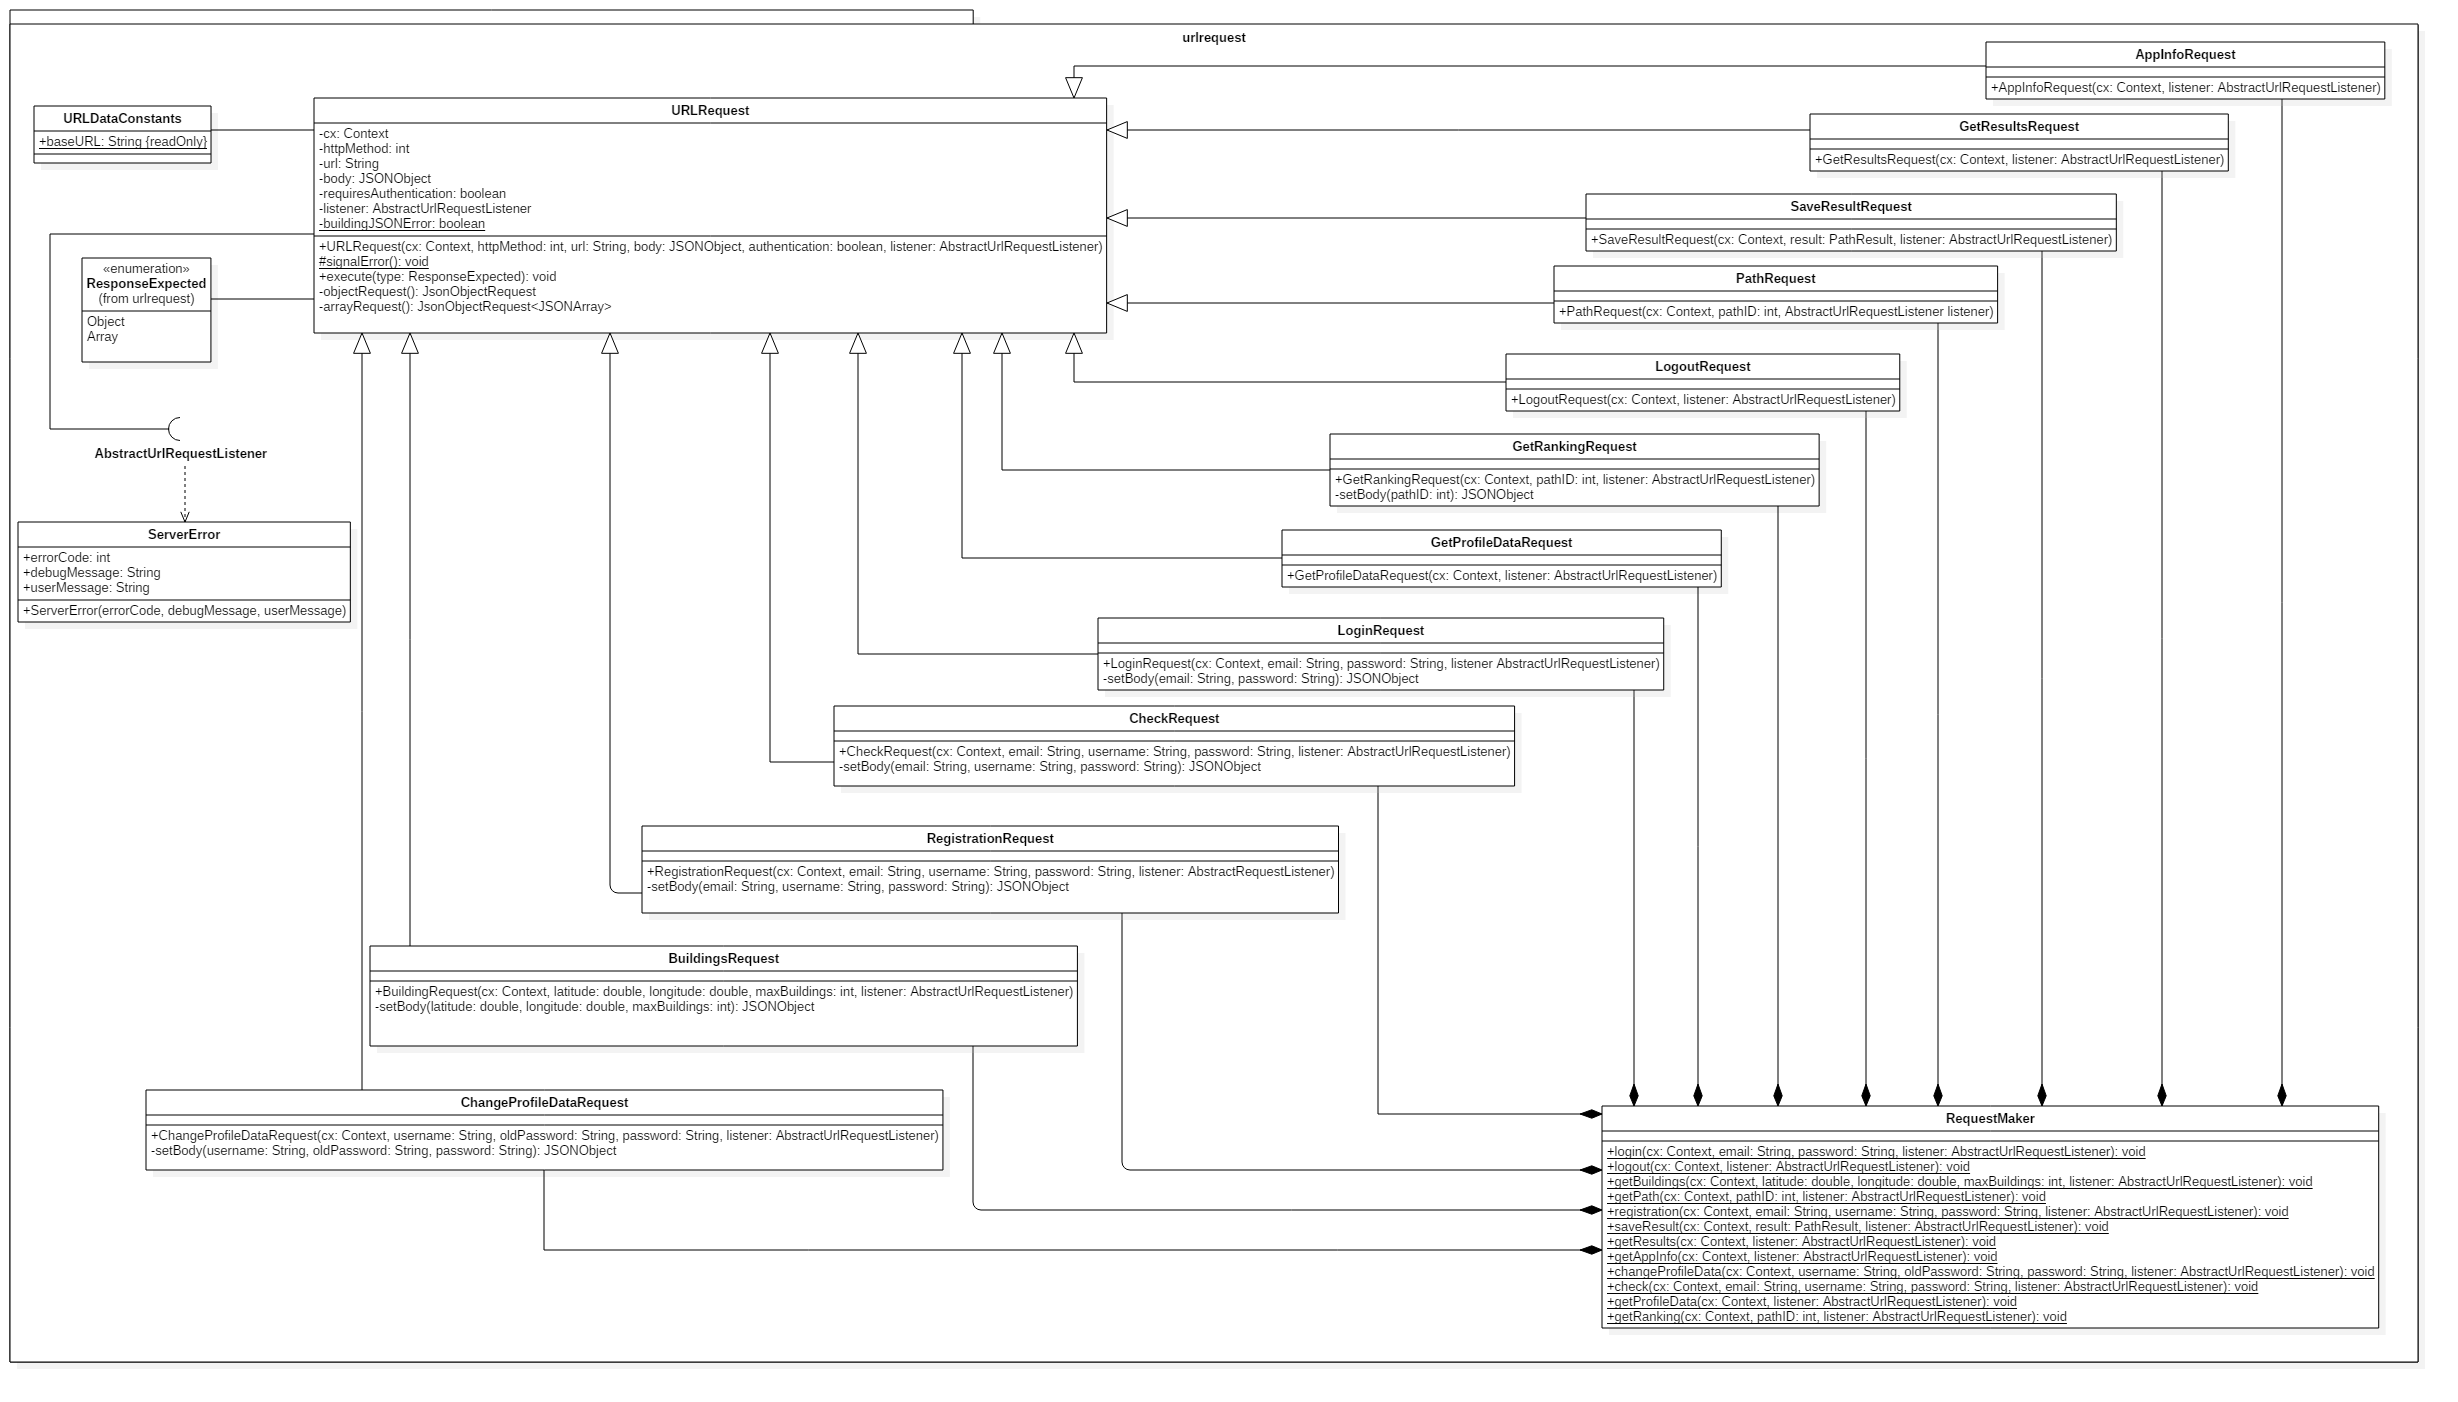
\includegraphics[scale=0.4]{img/package/png/client--urlrequest.png}
\caption{Schema package client::urlrequest}
 \end{figure}
\compDescrizione{componente che si occupa di effettuare le richieste al server}
\compPadre{data}
\begin{compClassi} \\
\begin{classe}{CLIPS::client::data::urlrequest::AbstractUrlRequestListener}
\classeDescrizione{interfaccia che definisce la struttura del listener astratto usato nel package urlrequest}
\classeUtilizzo{permette alle classi che interagiscono con l'urlrequest di definire un proprio listener concreto da poter usare per le chiamate al server}
\begin{classeMetodi}
\classeMetodo{onError}{error}{void}{Metodo chiamato quando viene inviato un errore al listener}
\begin{classeMetodoArgomenti}
\classeMetodoArgomento{error}{ServerError}{Contiene i dati relativi all'errore segnalato, quindi il codice e una spiegazione del tipo di errore avuto}
\end{classeMetodoArgomenti}
\classeMetodo{onResponse}{response}{void}{Metodo chiamato quando viene inviata la risposta al listener}
\begin{classeMetodoArgomenti}
\classeMetodoArgomento{response}{JSONObject}{Contiene i dati richiesti dal client}
\end{classeMetodoArgomenti}
\end{classeMetodi}
\begin{classeRelazioni}
\classeRelazione{CLIPS::client::data::urlrequest}{ServerError}{classe che rappresenta l'errore che il client riceve quando la richiesta al server non ha successo}\end{classeRelazioni}
\end{classe}\begin{classe}{CLIPS::client::data::urlrequest::AppInfoRequest}
\classeDescrizione{classe per la richiesta al server di dati sulle info dell'app, tra cui lo UUID dei beacon usati per l'applicazione e le informazioni sull'applicazione}
\classeUtilizzo{permette di effettuare una richiesta al server di dati sulle info dell'app}
\begin{classeRelazioni}
\classeRelazione{CLIPS::client::data::urlrequest}{AbstractUrlRequestListener}{interfaccia che definisce la struttura del listener astratto usato nel package urlrequest}\classeRelazione{CLIPS::client::data::urlrequest}{URLDataConstants}{classe che contiene i dati per effettuare le richieste al server che potrebbero variare nel tempo}\end{classeRelazioni}
\end{classe}\begin{classe}{CLIPS::client::data::urlrequest::BuildingsRequest}
\classeDescrizione{classe per la richiesta di dati sugli edifici}
\classeUtilizzo{permette di effettuare una richiesta al server di dati sugli edifici}
\begin{classeMetodi}
\classeMetodo{setBody}{latitude, longitude, maxBuildings}{JSONObject}{costruisce la sezione body dell'oggetto JSON, è un metodo di supporto}
\begin{classeMetodoArgomenti}
\classeMetodoArgomento{latitude}{double}{indica la latitudine attuale dell'utente, serve per trovare gli edifici più vicini}
\classeMetodoArgomento{longitude}{double}{indica la longitudine attuale dell'utente, serve per trovare gli edifici più vicini}
\classeMetodoArgomento{maxBuildings}{int}{indica il numero massimo di edifici richiesto, in questo modo si evita di richiedere liste troppo lunghe mantenendo allo stesso tempo la possibilità di visualizzare più risultati}
\end{classeMetodoArgomenti}
\end{classeMetodi}
\begin{classeRelazioni}
\classeRelazione{CLIPS::client::data::urlrequest}{AbstractUrlRequestListener}{interfaccia che definisce la struttura del listener astratto usato nel package urlrequest}\classeRelazione{CLIPS::client::data::urlrequest}{URLDataConstants}{classe che contiene i dati per effettuare le richieste al server che potrebbero variare nel tempo}\end{classeRelazioni}
\end{classe}\begin{classe}{CLIPS::client::data::urlrequest::ChangeProfileDataRequest}
\classeDescrizione{classe per la richiesta al server di cambiare i dati dell'utente}
\classeUtilizzo{permette di inviare la richiesta al server di cambiare i dati dell'utente, in particolare possono essere modificati solo lo username e la password}
\begin{classeMetodi}
\classeMetodo{setBody}{oldPassword, password}{JSONObject}{costruisce la sezione body dell'oggetto JSON, è un metodo di supporto}
\begin{classeMetodoArgomenti}
\classeMetodoArgomento{oldPassword}{string}{è la vecchia password dell'utente}
\classeMetodoArgomento{password}{string}{è la nuova password dell'utente}
\end{classeMetodoArgomenti}
\end{classeMetodi}
\begin{classeRelazioni}
\classeRelazione{CLIPS::client::data::urlrequest}{AbstractUrlRequestListener}{interfaccia che definisce la struttura del listener astratto usato nel package urlrequest}\classeRelazione{CLIPS::client::data::urlrequest}{URLDataConstants}{classe che contiene i dati per effettuare le richieste al server che potrebbero variare nel tempo}\end{classeRelazioni}
\end{classe}\begin{classe}{CLIPS::client::data::urlrequest::CheckRequest}
\classeDescrizione{classe per la richiesta al server del controllo dei dati inseriti dall'utente}
\classeUtilizzo{permette di inviare la richiesta al server per controllare se l'email, lo username o la password sono corretti}
\begin{classeMetodi}
\classeMetodo{setBody}{password, username}{JSONObject}{costruisce la sezione body dell'oggetto JSON, è un metodo di supporto}
\begin{classeMetodoArgomenti}
\classeMetodoArgomento{password}{string}{è la password digitata dall'utente}
\classeMetodoArgomento{username}{string}{è lo username digitato dall'utente}
\end{classeMetodoArgomenti}
\end{classeMetodi}
\begin{classeRelazioni}
\classeRelazione{CLIPS::client::data::urlrequest}{AbstractUrlRequestListener}{interfaccia che definisce la struttura del listener astratto usato nel package urlrequest}\classeRelazione{CLIPS::client::data::urlrequest}{URLDataConstants}{classe che contiene i dati per effettuare le richieste al server che potrebbero variare nel tempo}\end{classeRelazioni}
\end{classe}\begin{classe}{CLIPS::client::data::urlrequest::GetProfileDataRequest}
\classeDescrizione{classe per la richiesta al server di aggiornare in locale i dati dell'utente}
\classeUtilizzo{permette di inviare la richiesta al server per aggiornare l'email e lo username dell'utente nel caso non fossero uguali a quelli salvati nel server}
\begin{classeRelazioni}
\classeRelazione{CLIPS::client::data::urlrequest}{AbstractUrlRequestListener}{interfaccia che definisce la struttura del listener astratto usato nel package urlrequest}\classeRelazione{CLIPS::client::data::urlrequest}{URLDataConstants}{classe che contiene i dati per effettuare le richieste al server che potrebbero variare nel tempo}\end{classeRelazioni}
\end{classe}\begin{classe}{CLIPS::client::data::urlrequest::GetRankingRequest}
\classeDescrizione{classe per la richiesta al server dei dati sulla classifica di un determinato percorso}
\classeUtilizzo{permette di inviare la richiesta al server per ottenere i dati sulla classifica del percorso selezionato}
\begin{classeMetodi}
\classeMetodo{setBody}{pathID}{JSONObject}{costruisce la sezione body dell'oggetto JSON, è un metodo di supporto}
\begin{classeMetodoArgomenti}
\classeMetodoArgomento{pathID}{int}{l'ID del percorso per cui bisogna chiedere la classifica}
\end{classeMetodoArgomenti}
\end{classeMetodi}
\begin{classeRelazioni}
\classeRelazione{CLIPS::client::data::urlrequest}{AbstractUrlRequestListener}{interfaccia che definisce la struttura del listener astratto usato nel package urlrequest}\classeRelazione{CLIPS::client::data::urlrequest}{URLDataConstants}{classe che contiene i dati per effettuare le richieste al server che potrebbero variare nel tempo}\end{classeRelazioni}
\end{classe}\begin{classe}{CLIPS::client::data::urlrequest::GetResultsRequest}
\classeDescrizione{classe per la richiesta al server dei risultati salvati dall'utente in precedenza}
\classeUtilizzo{permette di effettuare la richiesta al server dei risultati salvati dall'utente in precedenza}
\begin{classeRelazioni}
\classeRelazione{CLIPS::client::data::urlrequest}{AbstractUrlRequestListener}{interfaccia che definisce la struttura del listener astratto usato nel package urlrequest}\classeRelazione{CLIPS::client::data::urlrequest}{URLDataConstants}{classe che contiene i dati per effettuare le richieste al server che potrebbero variare nel tempo}\end{classeRelazioni}
\end{classe}\begin{classe}{CLIPS::client::data::urlrequest::LoginRequest}
\classeDescrizione{classe per la richiesta di login al server}
\classeUtilizzo{permette di effettuare una richiesta di login al server}
\begin{classeMetodi}
\classeMetodo{setBody}{email, password}{JSONObject}{costruisce la sezione body dell'oggetto JSON, è un metodo di supporto}
\begin{classeMetodoArgomenti}
\classeMetodoArgomento{email}{string}{l'email inserita dall'utente per effettuare il login}
\classeMetodoArgomento{password}{string}{la password inserita dall'utente per effettuare il login}
\end{classeMetodoArgomenti}
\end{classeMetodi}
\begin{classeRelazioni}
\classeRelazione{CLIPS::client::data::urlrequest}{AbstractUrlRequestListener}{interfaccia che definisce la struttura del listener astratto usato nel package urlrequest}\classeRelazione{CLIPS::client::data::urlrequest}{URLDataConstants}{classe che contiene i dati per effettuare le richieste al server che potrebbero variare nel tempo}\end{classeRelazioni}
\end{classe}\begin{classe}{CLIPS::client::data::urlrequest::LogoutRequest}
\classeDescrizione{classe per la richiesta di logout al server}
\classeUtilizzo{permette di effettuare una richiesta di logout al server}
\begin{classeRelazioni}
\classeRelazione{CLIPS::client::data::urlrequest}{AbstractUrlRequestListener}{interfaccia che definisce la struttura del listener astratto usato nel package urlrequest}\classeRelazione{CLIPS::client::data::urlrequest}{URLDataConstants}{classe che contiene i dati per effettuare le richieste al server che potrebbero variare nel tempo}\end{classeRelazioni}
\end{classe}\begin{classe}{CLIPS::client::data::urlrequest::PathRequest}
\classeDescrizione{classe per la richiesta al server dei dati sul percorso selezionato, in particolare fornisce tutte le informazioni necessarie per poter svolgere il percorso}
\classeUtilizzo{permette di richiedere al server i dati sul percorso selezionato}
\begin{classeRelazioni}
\classeRelazione{CLIPS::client::data::urlrequest}{AbstractUrlRequestListener}{interfaccia che definisce la struttura del listener astratto usato nel package urlrequest}\classeRelazione{CLIPS::client::data::urlrequest}{URLDataConstants}{classe che contiene i dati per effettuare le richieste al server che potrebbero variare nel tempo}\end{classeRelazioni}
\end{classe}\begin{classe}{CLIPS::client::data::urlrequest::RegistrationRequest}
\classeDescrizione{classe per la richiesta di registrazione al server}
\classeUtilizzo{permette di effettuare una richiesta di registrazione al server}
\begin{classeMetodi}
\classeMetodo{setBody}{email, password, username}{JSONObject}{costruisce la sezione body dell'oggetto JSON, è un metodo di supporto}
\begin{classeMetodoArgomenti}
\classeMetodoArgomento{email}{string}{l'email inserita dall'utente per effettuare la registrazione}
\classeMetodoArgomento{password}{string}{la password inserita dall'utente per effettuare la registrazione}
\classeMetodoArgomento{username}{string}{lo username inserito dall'utente per effettuare la registrazione}
\end{classeMetodoArgomenti}
\end{classeMetodi}
\begin{classeRelazioni}
\classeRelazione{CLIPS::client::data::urlrequest}{AbstractUrlRequestListener}{interfaccia che definisce la struttura del listener astratto usato nel package urlrequest}\classeRelazione{CLIPS::client::data::urlrequest}{URLDataConstants}{classe che contiene i dati per effettuare le richieste al server che potrebbero variare nel tempo}\end{classeRelazioni}
\end{classe}\begin{classe}{CLIPS::client::data::urlrequest::RequestMaker}
\classeDescrizione{classe per la costruzione e l'invio di richieste al server, funziona come un'interfaccia dell'urlrequest per il resto dell'applicazione e quindi regola l'interazione con il package}
\classeUtilizzo{permette la costruzione e l'invio di richieste al server}
\begin{classeMetodi}
\classeMetodo{changeProfileData}{cx, listener, oldPassword, password, username}{void}{crea l'oggetto per chiedere al server di verificare e cambiare i dati inseriti dall'utente}
\begin{classeMetodoArgomenti}
\classeMetodoArgomento{cx}{Context}{è una classe delle librerie base di Android che costituisce il cuore dell'applicazione, e quindi è necessaria per poter effettuare alcune operazioni, tra cui le richieste al server}
\classeMetodoArgomento{listener}{AbstractUrlRequestListener}{il listener che verrà usato per informare l'applicazione se la richiesta al server ha avuto successo o meno}
\classeMetodoArgomento{oldPassword}{string}{la vecchia password, richiesta e digitata dall'utente per evitare cambi di dati a sua insaputa}
\classeMetodoArgomento{password}{string}{la nuovo password digitata dall'utente}
\classeMetodoArgomento{username}{string}{il nuovo username digitato dall'utente}
\end{classeMetodoArgomenti}
\classeMetodo{check}{cx, email, listener, password, username}{void}{crea l'oggetto per chiedere al server di verificare se i dati inseriti dall'utente sono validi}
\begin{classeMetodoArgomenti}
\classeMetodoArgomento{cx}{Context}{è una classe delle librerie base di Android che costituisce il cuore dell'applicazione, e quindi è necessaria per poter effettuare alcune operazioni, tra cui le richieste al server}
\classeMetodoArgomento{email}{string}{l'indirizzo email inserito dall'utente}
\classeMetodoArgomento{listener}{AbstractUrlRequestListener}{il listener che verrà usato per informare l'applicazione se la richiesta al server ha avuto successo o meno}
\classeMetodoArgomento{password}{string}{la password inserita dall'utente}
\classeMetodoArgomento{username}{string}{lo usernamel inserito dall'utente}
\end{classeMetodoArgomenti}
\classeMetodo{getAppInfo}{cx, listener}{void}{crea l'oggetto per ottenere dal server le informazioni sull'applicazione}
\begin{classeMetodoArgomenti}
\classeMetodoArgomento{cx}{Context}{è una classe delle librerie base di Android che costituisce il cuore dell'applicazione, e quindi è necessaria per poter effettuare alcune operazioni, tra cui le richieste al server}
\classeMetodoArgomento{listener}{AbstractUrlRequestListener}{il listener che verrà usato per informare l'applicazione se la richiesta al server ha avuto successo o meno}
\end{classeMetodoArgomenti}
\classeMetodo{getBuildings}{cx, latitude, listener, longitude, maxBuildings}{void}{crea l'oggetto per ottenere dal server i dati degli edifici abilitati più vicini alla sua posizione}
\begin{classeMetodoArgomenti}
\classeMetodoArgomento{cx}{Context}{è una classe delle librerie base di Android che costituisce il cuore dell'applicazione, e quindi è necessaria per poter effettuare alcune operazioni, tra cui le richieste al server}
\classeMetodoArgomento{latitude}{double}{la latitudine dell'utente, viene usata per trovare gli edifici più vicini a lui}
\classeMetodoArgomento{listener}{AbstractUrlRequestListener}{il listener che verrà usato per informare l'applicazione se la richiesta al server ha avuto successo o meno}
\classeMetodoArgomento{longitude}{double}{la longitudine dell'utente, viene usata per trovare gli edifici più vicini a lui}
\classeMetodoArgomento{maxBuildings}{int}{il numero massimo di edifici richiesti, viene usato per non dover inviare inutilmente i dati di tutti gli edifici}
\end{classeMetodoArgomenti}
\classeMetodo{getPath}{cx, listener, pathID}{void}{crea l'oggetto per ottenere dal server i dati del percorso selezionato}
\begin{classeMetodoArgomenti}
\classeMetodoArgomento{cx}{Context}{è una classe delle librerie base di Android che costituisce il cuore dell'applicazione, e quindi è necessaria per poter effettuare alcune operazioni, tra cui le richieste al server}
\classeMetodoArgomento{listener}{AbstractUrlRequestListener}{il listener che verrà usato per informare l'applicazione se la richiesta al server ha avuto successo o meno}
\classeMetodoArgomento{pathID}{int}{l'ID del percorso, verrà usato dal server per capire quale percorso è stato selezionato}
\end{classeMetodoArgomenti}
\classeMetodo{getProfileData}{cx, listener}{void}{crea l'oggetto per ottenere dal server i dati attuali del profilo dell'utente}
\begin{classeMetodoArgomenti}
\classeMetodoArgomento{cx}{Context}{è una classe delle librerie base di Android che costituisce il cuore dell'applicazione, e quindi è necessaria per poter effettuare alcune operazioni, tra cui le richieste al server}
\classeMetodoArgomento{listener}{AbstractUrlRequestListener}{il listener che verrà usato per informare l'applicazione se la richiesta al server ha avuto successo o meno}
\end{classeMetodoArgomenti}
\classeMetodo{getRanking}{cx, listener, pathID}{void}{crea la classe per ottenere dal server i dati sulla classifica del percorso selzionato}
\begin{classeMetodoArgomenti}
\classeMetodoArgomento{cx}{Context}{è una classe delle librerie base di Android che costituisce il cuore dell'applicazione, e quindi è necessaria per poter effettuare alcune operazioni, tra cui le richieste al server}
\classeMetodoArgomento{listener}{AbstractUrlRequestListener}{il listener che verrà usato per informare l'applicazione se la richiesta al server ha avuto successo o meno}
\classeMetodoArgomento{pathID}{int}{l'id del percorso selezionato dall'utente per ottenere la relativa classifica}
\end{classeMetodoArgomenti}
\classeMetodo{getResults}{cx, listener}{void}{crea l'oggetto per ottenere dal server i risultati conseguiti dall'utente}
\begin{classeMetodoArgomenti}
\classeMetodoArgomento{cx}{Context}{� una classe delle librerie base di Android che costituisce il cuore dell'applicazione, e quindi � necessaria per poter effettuare alcune operazioni, tra cui le richieste al server}
\classeMetodoArgomento{listener}{AbstractUrlRequestListener}{il listener che verr�� usato per informare l'applicazione se la richiesta al server ha avuto successo o meno}
\end{classeMetodoArgomenti}
\classeMetodo{login}{cx, email, listener, password}{void}{crea l'oggetto per chiedere al server di verificare i dati inseriti dall'utente per il login}
\begin{classeMetodoArgomenti}
\classeMetodoArgomento{cx}{Context}{è una classe delle librerie base di Android che costituisce il cuore dell'applicazione, e quindi è necessaria per poter effettuare alcune operazioni, tra cui le richieste al server}
\classeMetodoArgomento{email}{string}{l'indirizzo email inserito dall'utente per effettuare il login}
\classeMetodoArgomento{listener}{AbstractUrlRequestListener}{il listener che verrà usato per informare l'applicazione se la richiesta al server ha avuto successo o meno}
\classeMetodoArgomento{password}{string}{la passwordl inserita dall'utente per effettuare il login}
\end{classeMetodoArgomenti}
\classeMetodo{logout}{cx, listener}{void}{crea l'oggetto per notificare al server che l'utente ha effettuato il logout}
\begin{classeMetodoArgomenti}
\classeMetodoArgomento{cx}{Context}{è una classe delle librerie base di Android che costituisce il cuore dell'applicazione, e quindi è necessaria per poter effettuare alcune operazioni, tra cui le richieste al server}
\classeMetodoArgomento{listener}{AbstractUrlRequestListener}{il listener che verrà usato per informare l'applicazione se la richiesta al server ha avuto successo o meno}
\end{classeMetodoArgomenti}
\classeMetodo{registration}{cx, email, listener, password, username}{void}{crea l'oggetto per chiedere al server di verificare e registrare il profilo inserito dall'utente}
\begin{classeMetodoArgomenti}
\classeMetodoArgomento{cx}{Context}{è una classe delle librerie base di Android che costituisce il cuore dell'applicazione, e quindi è necessaria per poter effettuare alcune operazioni, tra cui le richieste al server}
\classeMetodoArgomento{email}{string}{l'indirizzo email che l'utente ha inserito per registrarsi}
\classeMetodoArgomento{listener}{AbstractUrlRequestListener}{il listener che verrà usato per informare l'applicazione se la richiesta al server ha avuto successo o meno}
\classeMetodoArgomento{password}{string}{la password che l'utente ha inserito per registrarsi}
\classeMetodoArgomento{username}{string}{lo username che l'utente ha inserito per registrarsi}
\end{classeMetodoArgomenti}
\classeMetodo{saveResult}{cx, listener, result}{void}{crea l'oggetto per salvare nel server il risultato appena ottenuto}
\begin{classeMetodoArgomenti}
\classeMetodoArgomento{cx}{Context}{è una classe delle librerie base di Android che costituisce il cuore dell'applicazione, e quindi è necessaria per poter effettuare alcune operazioni, tra cui le richieste al server}
\classeMetodoArgomento{listener}{AbstractUrlRequestListener}{il listener che verrà usato per informare l'applicazione se la richiesta al server ha avuto successo o meno}
\classeMetodoArgomento{result}{PathResult}{l'oggetto che contiene i risultati da salvare nel server}
\end{classeMetodoArgomenti}
\end{classeMetodi}
\begin{classeRelazioni}
\classeRelazione{CLIPS::client::data::urlrequest}{AbstractUrlRequestListener}{interfaccia che definisce la struttura del listener astratto usato nel package urlrequest}\classeRelazione{CLIPS::client::data::urlrequest}{AppInfoRequest}{classe per la richiesta al server di dati sulle info dell'app, tra cui lo UUID dei beacon usati per l'applicazione e le informazioni sull'applicazione}\classeRelazione{CLIPS::client::data::urlrequest}{BuildingsRequest}{classe per la richiesta di dati sugli edifici}\classeRelazione{CLIPS::client::data::urlrequest}{ChangeProfileDataRequest}{classe per la richiesta al server di cambiare i dati dell'utente}\classeRelazione{CLIPS::client::data::urlrequest}{CheckRequest}{classe per la richiesta al server del controllo dei dati inseriti dall'utente}\classeRelazione{CLIPS::client::data::urlrequest}{GetProfileDataRequest}{classe per la richiesta al server di aggiornare in locale i dati dell'utente}\classeRelazione{CLIPS::client::data::urlrequest}{GetRankingRequest}{classe per la richiesta al server dei dati sulla classifica di un determinato percorso}\classeRelazione{CLIPS::client::data::urlrequest}{GetResultsRequest}{classe per la richiesta al server dei risultati salvati dall'utente in precedenza}\classeRelazione{CLIPS::client::data::urlrequest}{LoginRequest}{classe per la richiesta di login al server}\classeRelazione{CLIPS::client::data::urlrequest}{LogoutRequest}{classe per la richiesta di logout al server}\classeRelazione{CLIPS::client::data::urlrequest}{PathRequest}{classe per la richiesta al server dei dati sul percorso selezionato, in particolare fornisce tutte le informazioni necessarie per poter svolgere il percorso}\classeRelazione{CLIPS::client::data}{PathResult}{classe che rappresenta i risultati di un percorso}\classeRelazione{CLIPS::client::data::urlrequest}{RegistrationRequest}{classe per la richiesta di registrazione al server}\classeRelazione{CLIPS::client::data::urlrequest}{SaveResultRequest}{classe per la richiesta al server di salvataggio del risultato del percorso appena finito}\end{classeRelazioni}
\end{classe}\begin{classe}{CLIPS::client::data::urlrequest::SaveResultRequest}
\classeDescrizione{classe per la richiesta al server di salvataggio del risultato del percorso appena finito}
\classeUtilizzo{permette di effettuare una richiesta al server di salvataggio del risultato del percorso appena finito}
\begin{classeMetodi}
\classeMetodo{setBody}{result}{JSONObject}{costruisce la sezione body dell'oggetto JSON, è un metodo di supporto}
\begin{classeMetodoArgomenti}
\classeMetodoArgomento{result}{PathResult}{il risultato da salvare nel server}
\end{classeMetodoArgomenti}
\end{classeMetodi}
\begin{classeRelazioni}
\classeRelazione{CLIPS::client::data::urlrequest}{AbstractUrlRequestListener}{interfaccia che definisce la struttura del listener astratto usato nel package urlrequest}\classeRelazione{CLIPS::client::data}{PathResult}{classe che rappresenta i risultati di un percorso}\classeRelazione{CLIPS::client::data}{ProofResult}{classe che rappresenta il risultato di una prova}\classeRelazione{CLIPS::client::data::urlrequest}{URLDataConstants}{classe che contiene i dati per effettuare le richieste al server che potrebbero variare nel tempo}\end{classeRelazioni}
\end{classe}\begin{classe}{CLIPS::client::data::urlrequest::ServerError}
\classeDescrizione{classe che rappresenta l'errore che il client riceve quando la richiesta al server non ha successo}
\classeUtilizzo{permette di rappresentare l'errore ricevuto in una forma più semplice da usare nel resto dell'applicazione}
\begin{classeAttributi}
\classeAttributo{debugMessage}{string}{il messaggio destinato agli sviluppatori, per aiutarli ad individuare dove è avvenuto l'errore}
\classeAttributo{errorCode}{int}{il codice dell'errore segnalato}
\classeAttributo{userMessage}{string}{il messaggio destinato all'utente, per comunicargli che l'applicazione ha riscontrato un errore}
\end{classeAttributi}
\end{classe}\begin{classe}{CLIPS::client::data::urlrequest::URLDataConstants}
\classeDescrizione{classe che contiene i dati per effettuare le richieste al server che potrebbero variare nel tempo}
\classeUtilizzo{permette di gestire facilmente eventuali cambiamenti futuri dei dati necessari ad effettuare le richieste al server}
\begin{classeAttributi}
\classeAttributo{baseURL}{string}{Contiene l'url del server, facilita l'aggiornamento del client a seguito di modifiche del server}
\end{classeAttributi}
\end{classe}\begin{classe}{CLIPS::client::data::urlrequest::URLRequest}
\classeDescrizione{classe che si occupa delle richieste da inviare al server, fornisce un'implementazione delle richieste in base ai dati forniti alle sue classi derivate}
\classeUtilizzo{permette di effettuare tutte le richieste al server necessarie per far funzionare l'applicazione}
\begin{classeAttributi}
\classeAttributo{body}{JSONObject}{è la parte della richiesta al server che contiene i dati necessari per portare a compimento la chiamata}
\classeAttributo{buildingJSONError}{bool}{valore booleno che indica se è avvenuto o meno un errore durante la costruzione del body, viene impostato dalle classi derivate di URLRequest}
\classeAttributo{cx}{Context}{è una classe delle librerie base di Android che costituisce il cuore dell'applicazione, e quindi è necessaria per poter effettuare alcune operazioni, tra cui le richieste al server}
\classeAttributo{httpMethod}{int}{è un'enumerazione che indica quale metodo HTTP eseguire, di fatto gli unici valori usati sono GET e POST}
\classeAttributo{listener}{AbstractUrlRequestListener}{il listener che verrà usato per informare l'applicazione se la richiesta al server ha avuto successo o meno}
\classeAttributo{requiresAuthentication}{bool}{indica se la chiamata necessita di aggiungere il token salvato all'header dell'oggetto inviato}
\classeAttributo{url}{string}{l'url completo a cui mandare la richiesta}
\end{classeAttributi}
\begin{classeMetodi}
\classeMetodo{arrayRequest}{}{JsonRequest<JSONArray>}{è un metodo di supporto che crea una chiamata la cui risposta è un array JSON}
\classeMetodo{execute}{type}{void}{crea ed esegue la chiamata al server in base ai campi dati salvati}
\begin{classeMetodoArgomenti}
\classeMetodoArgomento{type}{ResponseExpected}{indica se la chiamata si aspetta di ricevere, in caso di successo, un oggetto o un array JSON}
\end{classeMetodoArgomenti}
\classeMetodo{objectRequest}{}{JSONObjectRequest}{è un metodo di supporto che crea una chiamata la cui risposta è un oggetto JSON}
\classeMetodo{signalError}{}{void}{cambia il valore di buildingJSONError in \texttt{true} e segnala quindi all'URLRequest che c'è stato un errore in fase di costruzione di ''body'', viene invocato dalle classi derivate di URLRequest}
\end{classeMetodi}
\begin{classeRelazioni}
\classeRelazione{CLIPS::client::data::urlrequest}{AbstractUrlRequestListener}{interfaccia che definisce la struttura del listener astratto usato nel package urlrequest}\classeRelazione{CLIPS::client::data::datamanager}{LoginManager}{classe che gestisce le operazioni del profilo dell'utente}\classeRelazione{CLIPS::client::data::urlrequest}{ServerError}{classe che rappresenta l'errore che il client riceve quando la richiesta al server non ha successo}\end{classeRelazioni}
\end{classe}\end{compClassi}
\end{componente}
\begin{componente}{CLIPS::client::pathprogress}
\begin{figure}[h!]
\centering
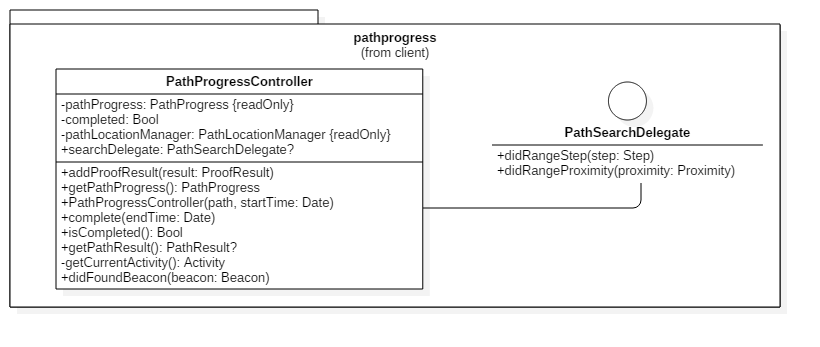
\includegraphics[scale=0.4]{img/package/png/client--pathprogress.png}
\caption{Schema package client::pathprogress}
 \end{figure}
\compDescrizione{componente che gestisce i dati del percorso e salva i risultati ottenuti nelle prove mentre si sta giocando}
\compPadre{client}
\begin{compClassi} \\
\begin{classe}{CLIPS::client::pathprogress::BeaconDiscover}
\classeDescrizione{classe che si interfaccia direttamente con i beacon fisici}
\classeUtilizzo{permette di rilevare i beacon}
\begin{classeAttributi}
\classeAttributo{delegate}{BeaconDiscoverDelegate}{riferimento al delegate}
\end{classeAttributi}
\end{classe}\begin{classe}{CLIPS::client::pathprogress::BeaconDiscoverDelegate}
\classeDescrizione{interfaccia utilizzata per notificare se il dispositivo è entrato o uscito dal raggio di un beacon}
\classeUtilizzo{permette di notificare se si è entrati o usciti dal raggio di un beacon}
\begin{classeMetodi}
\classeMetodo{didFoundBeacon}{rawBeacon}{void}{segnala quando è stato trovato un beacon}
\begin{classeMetodoArgomenti}
\classeMetodoArgomento{rawBeacon}{RawBeacon}{rappresenta un beacon fisico}
\end{classeMetodoArgomenti}
\classeMetodo{didMoveFromBeacon}{rawBeacon}{void}{segnala che si è usciti dal raggio di un beacon}
\begin{classeMetodoArgomenti}
\classeMetodoArgomento{rawBeacon}{RawBeacon}{rappresenta un beacon fisico}
\end{classeMetodoArgomenti}
\end{classeMetodi}
\begin{classeRelazioni}
\classeRelazione{CLIPS::client::pathprogress}{PathProgressController}{classe che gestisce l'avanzamento di un percorso}\end{classeRelazioni}
\end{classe}\begin{classe}{CLIPS::client::pathprogress::PathProgressController}
\classeDescrizione{classe che gestisce l'avanzamento di un percorso}
\classeUtilizzo{permette di gestire i dati dell'avanzamento di un percorso}
\begin{classeAttributi}
\classeAttributo{delegate}{PathProgressControllerDelegate}{riferimento al delegate}
\classeAttributo{path}{Path}{rappresenta un il path di cui deve gestire l'avanzamento}
\classeAttributo{pathProgress}{PathProgress}{rappresenta il path progress nel database locale}
\classeAttributo{rawBeacons}{Vector<RawBeacon>}{rappresenta un vettore di raw beacon}
\end{classeAttributi}
\begin{classeMetodi}
\classeMetodo{addProofResult}{result}{void}{aggiunge un risultato di una prova nel database locale}
\begin{classeMetodoArgomenti}
\classeMetodoArgomento{result}{ProofResult}{risultato da aggiungere}
\end{classeMetodoArgomenti}
\classeMetodo{didFoundBeacon}{rawBeacon}{void}{implementazione del metodo dell'interfaccia che stabilisce cosa fare quando viene trovato un beacon}
\begin{classeMetodoArgomenti}
\classeMetodoArgomento{rawBeacon}{RawBeacon}{rappresenta un beacon fisico}
\end{classeMetodoArgomenti}
\classeMetodo{didMoveFromBeacon}{rawBeacon}{void}{implementazione del metodo dell'interfaccia che stabilisce cosa fare qualora si esca dal raggio di un beacon}
\begin{classeMetodoArgomenti}
\classeMetodoArgomento{rawBeacon}{RawBeacon}{rappresenta un beacon fisico}
\end{classeMetodoArgomenti}
\classeMetodo{getPathProgress}{}{PathProgress}{ritorna il pathprogress}
\end{classeMetodi}
\begin{classeRelazioni}
\classeRelazione{CLIPS::client::pathprogress}{BeaconDiscoverDelegate}{interfaccia utilizzata per notificare se il dispositivo è entrato o uscito dal raggio di un beacon}\classeRelazione{CLIPS::client::data}{PathProgress}{classe per il salvataggio in locale del progresso di un percorso}\classeRelazione{CLIPS::client::pathprogress}{PathProgressControllerDelegate}{interfaccia utilizzata per notificare se si è in presenza del beacon del prossimo step o di uno del proximity}\classeRelazione{CLIPS::client::pathprogress}{RawBeacon}{classe che rappresenta un beacon semplice}\end{classeRelazioni}
\end{classe}\begin{classe}{CLIPS::client::pathprogress::PathProgressControllerDelegate}
\classeDescrizione{interfaccia utilizzata per notificare se si è in presenza del beacon del prossimo step o di uno del proximity}
\classeUtilizzo{notifica se si nel raggio del beacon del prossimo step o di uno di proximity}
\begin{classeMetodi}
\classeMetodo{didRangeProximity}{proximity}{void}{segnala che si è nel raggio di un beacon del proximity}
\begin{classeMetodoArgomenti}
\classeMetodoArgomento{proximity}{Proximity}{rappresenta il proximity nel quale ci si trova}
\end{classeMetodoArgomenti}
\classeMetodo{didReachStep}{step}{void}{segnala che si è nel raggio del beacon del prossimo step}
\begin{classeMetodoArgomenti}
\classeMetodoArgomento{step}{Step}{rappresenta il step in cui ci si trova}
\end{classeMetodoArgomenti}
\end{classeMetodi}
\end{classe}\begin{classe}{CLIPS::client::pathprogress::RawBeacon}
\classeDescrizione{classe che rappresenta un beacon semplice}
\classeUtilizzo{utilizzato per rappresentare un beacon fisico}
\begin{classeAttributi}
\classeAttributo{major}{int}{rappresenta il major del beacon fisico}
\classeAttributo{minor}{int}{rappresenta il minor del beacon fisico}
\classeAttributo{UUID}{string}{rappresenta l'UUID del beacon fisico}
\end{classeAttributi}
\end{classe}\end{compClassi}
\end{componente}
\begin{componente}{CLIPS::client::viewcontroller}
\begin{figure}[h!]
\centering
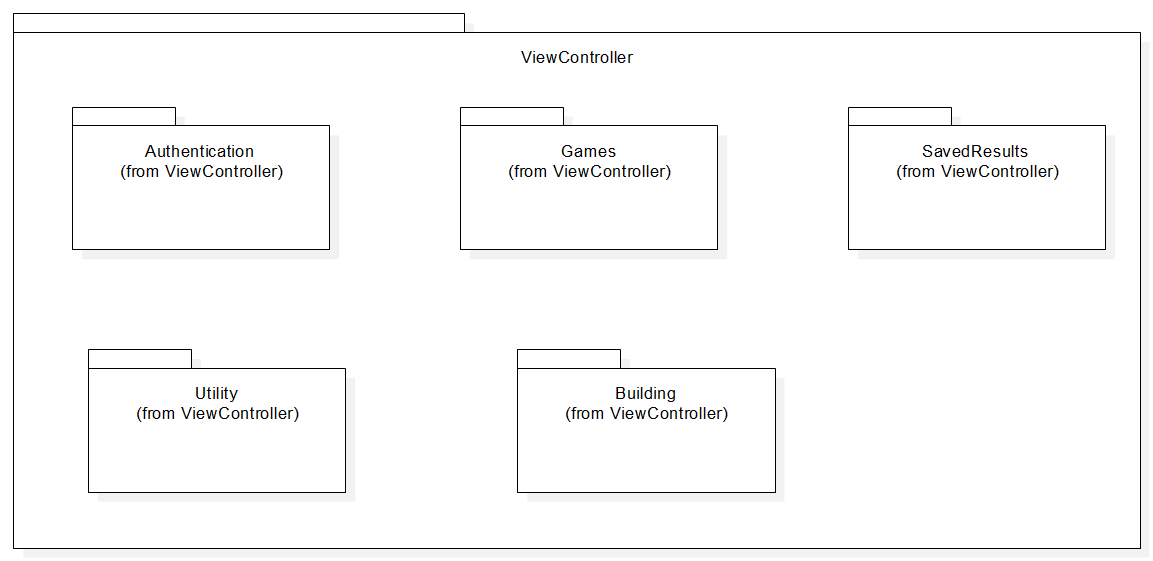
\includegraphics[scale=0.4]{img/package/png/client--viewcontroller.png}
\caption{Schema package client::viewcontroller}
 \end{figure}
\compDescrizione{componente che raggruppa tutte le view ed i controller relativi alle view}
\compPadre{client}
\begin{compPackageContenuti}
\item \texttt{CLIPS::client::viewcontroller::authentication}: componente che si occupa di gestire l'autenticazione dell'utente
\item \texttt{CLIPS::client::viewcontroller::building}: componente che gestisce le informazioni e le interazioni dell'utente con gli edifici abilitati
\item \texttt{CLIPS::client::viewcontroller::games}: componente che gestisce le prove che l'utente deve completare all'interno di un percorso
\item \texttt{CLIPS::client::viewcontroller::savedresults}: componente che raggruppa le le view e i controller dei risultati salvati e delle classifiche
\item \texttt{CLIPS::client::viewcontroller::utility}: componente che raggruppa le view generali dell'app
\end{compPackageContenuti}
\end{componente}
\begin{componente}{CLIPS::client::viewcontroller::authentication}
	\begin{figure}[h!]
		\centering
		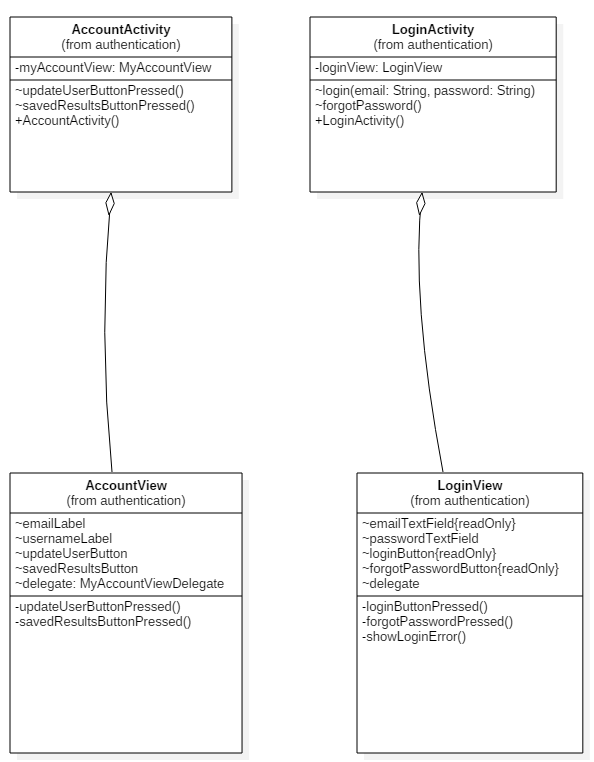
\includegraphics[scale=0.4]{img/package/png/client--viewcontroller--authentication1.png}
		\caption{Prima parte schema package client::viewcontroller::authentication}
	\end{figure}
	\begin{figure}[h!]
		\centering
		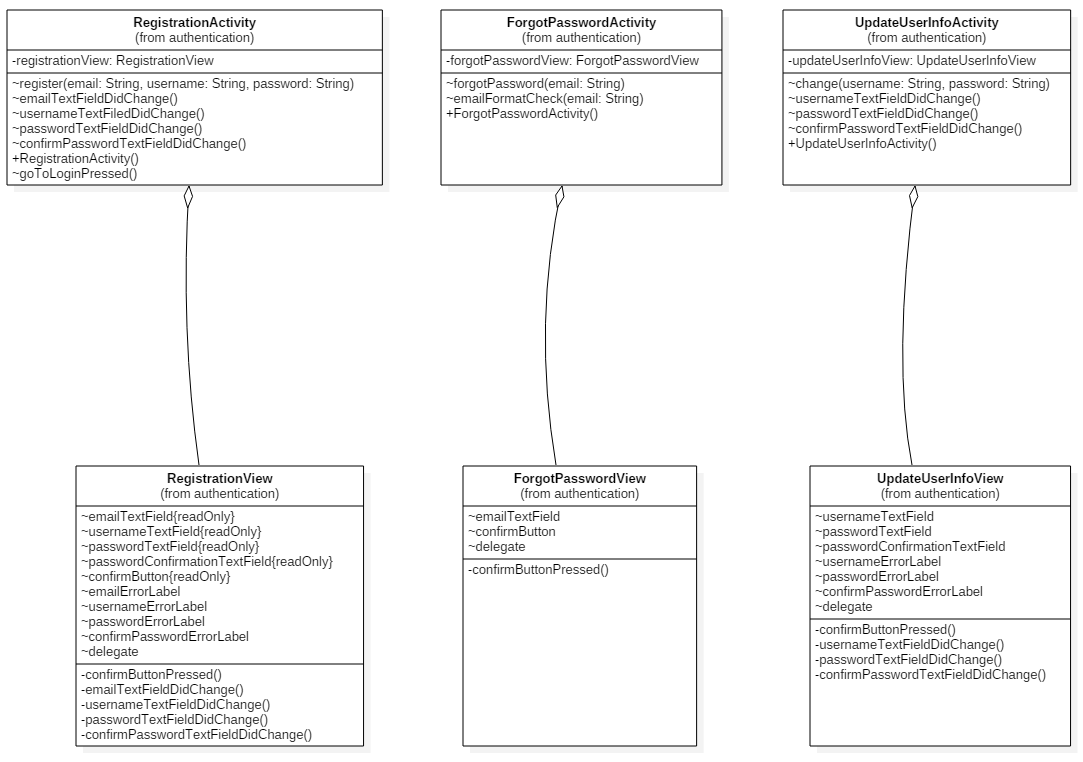
\includegraphics[scale=0.4]{img/package/png/client--viewcontroller--authentication2.png}
		\caption{Seconda parte schema package client::viewcontroller::authentication}
	\end{figure}
	\compDescrizione{componente che si occupa di gestire l'autenticazione dell'utente}
	\compPadre{client}
	\begin{compClassi} \\
		\begin{classe}{CLIPS::client::viewcontroller::authentication::AccountActivity}
			\classeDescrizione{classe controller che si occupa di interagire con AccountView}
			\classeUtilizzo{si occupa di gestire le interazioni dell'utente con AccountView}
			\begin{classeMetodi}
				\classeMetodo{onCreate}{}{void}{si occupa di inizializzare l'activity con la relativa view}
				\classeMetodo{setButtons}{}{void}{si occupa di inizializzare i collegamenti dei bottoni presenti nella view}
			\end{classeMetodi}
		\end{classe}\begin{classe}{CLIPS::client::viewcontroller::authentication::AccountView}
		\classeDescrizione{classe che rappresenta la schermata delle informazioni dell'utente}
		\classeUtilizzo{permette all'utente di visualizzare le informazioni del proprio profilo}
		\begin{classeAttributi}
			\classeAttributo{emailLabel}{TextView}{rappresenta l'email dell'utente}
			\classeAttributo{savedResultsButton}{Button}{rappresenta il bottone per visualizzare i risultati salvati}
			\classeAttributo{updateUserButton}{Button}{rappresenta il bottone per modificare le informazioni dell'utente}
			\classeAttributo{usernameLabel}{TextView}{indica l'username dell'utente}
		\end{classeAttributi}
		\begin{classeRelazioni}
			\classeRelazione{CLIPS::client::viewcontroller::authentication}{AccountActivity}{classe controller che si occupa di interagire con AccountView}\end{classeRelazioni}
	\end{classe}\begin{classe}{CLIPS::client::viewcontroller::authentication::ConfirmRegistration}
	\classeDescrizione{classe che interagisce con RegistrationActivity e permette all'utente di visualizzare i propri dati di registrazione}
	\classeUtilizzo{l'utente può visualizzare i dati inseriti in precedenza}
	\begin{classeRelazioni}
		\classeRelazione{CLIPS::client::viewcontroller::authentication}{RegistrationActivity}{classe controller che si occupa di interagire con RegistrationView}\end{classeRelazioni}
\end{classe}\begin{classe}{CLIPS::client::viewcontroller::authentication::ForgotPasswordActivity}
\classeDescrizione{classe controller che si occupa di interagire con ForgotPasswordView}
\classeUtilizzo{si occupa di gestire le interazioni dell'utente con ForgotPasswordView}
\begin{classeMetodi}
	\classeMetodo{onCreate}{SavedBundleInstance, savedInstanceState}{void}{si occupa di inizializzare l'activity con la relativa view}
	\begin{classeMetodoArgomenti}
		\classeMetodoArgomento{SavedBundleInstance}{Bundle}{contiene i dati dell'istanza creata o di un'attività precedente}
		\classeMetodoArgomento{savedInstanceState}{Bundle}{contiene i dati dell'istanza creata o di un'attività precedente}
	\end{classeMetodoArgomenti}
\end{classeMetodi}
\begin{classeRelazioni}
	\classeRelazione{CLIPS::client::viewcontroller::authentication}{ForgotPasswordView}{classe che si occupa della visualizzazione della schermata per la richiesta di una nuova password}\end{classeRelazioni}
\end{classe}\begin{classe}{CLIPS::client::viewcontroller::authentication::ForgotPasswordView}
\classeDescrizione{classe che si occupa della visualizzazione della schermata per la richiesta di una nuova password}
\classeUtilizzo{consente all'utente di inserire la mail per ricevere una nuova password}
\begin{classeAttributi}
	\classeAttributo{confirmButton}{Button}{rappresenta il bottone per la conferma dell'email inserita}
	\classeAttributo{emailTextField}{EditText}{rappresenta l'email da inserire da parte dell'utente}
\end{classeAttributi}
\end{classe}\begin{classe}{CLIPS::client::viewcontroller::authentication::LoginActivity}
\classeDescrizione{classe controller che si occupa di interagire con LoginView}
\classeUtilizzo{si occupa di gestire le interazioni dell'utente con LoginView}
\begin{classeMetodi}
	\classeMetodo{setButtons}{}{void}{si occupa di inizializzare i collegamenti dei bottoni presenti nella view}
\end{classeMetodi}
\begin{classeRelazioni}
	\classeRelazione{CLIPS::client::viewcontroller::authentication}{LoginView}{classe che si occupa della visualizzazione della schermata per il login}\end{classeRelazioni}
\end{classe}\begin{classe}{CLIPS::client::viewcontroller::authentication::LoginView}
\classeDescrizione{classe che si occupa della visualizzazione della schermata per il login}
\classeUtilizzo{consente all'utente di inserire i propri dati per effettuare il login}
\begin{classeAttributi}
	\classeAttributo{emailTextField}{EditText}{rappresenta l'email da inserire da parte dell'utente}
	\classeAttributo{forgotPasswordButton}{Button}{rappresenta il button per la password dimenticata}
	\classeAttributo{loginButton}{Button}{indica il button per effettuare il login}
	\classeAttributo{passwordTextField}{EditText}{rappresenta la password da inserire da parte dell'utente}
\end{classeAttributi}
\begin{classeMetodi}
	\classeMetodo{forgotPasswordPressed}{}{void}{invia un evento il quale notifica che il bottone di password dimenticata è stato premuto}
	\classeMetodo{loginButtonPressed}{}{void}{invia un evento di bottone del login premuto}
\end{classeMetodi}
\end{classe}\begin{classe}{CLIPS::client::viewcontroller::authentication::RecoverPassword}
\classeDescrizione{classe che rappresenta l'avvenuto recupero della password di un utente}
\classeUtilizzo{view che permette all'utente di sapere che la sua password è stata recuperata correttamente}
\end{classe}\begin{classe}{CLIPS::client::viewcontroller::authentication::RegistrationActivity}
\classeDescrizione{classe controller che si occupa di interagire con RegistrationView}
\classeUtilizzo{si occupa di gestire le interazioni dell'utente con RegistrationView}
\begin{classeMetodi}
	\classeMetodo{checkFields}{}{bool}{si occupa di controllare che i campi inseriti siano corretti}
	\classeMetodo{clearFields}{}{void}{questo metodo si occupa di resettare i campi dati presenti nella relativa view}
	\classeMetodo{onCreate}{SavedBundleInstance}{void}{si occupa di inizializzare l'activity con la relativa view}
	\begin{classeMetodoArgomenti}
		\classeMetodoArgomento{SavedBundleInstance}{Bundle}{contiene i dati dell'istanza creata o di un'attività precedente}
	\end{classeMetodoArgomenti}
	\classeMetodo{setButtons}{}{void}{si occupa di inizializzare i collegamenti dei bottoni presenti nella view
	}
\end{classeMetodi}
\begin{classeRelazioni}
	\classeRelazione{CLIPS::client::viewcontroller::authentication}{RegistrationView}{classe che si occupa della visualizzazione della schermata per la registrazione}\end{classeRelazioni}
\end{classe}\begin{classe}{CLIPS::client::viewcontroller::authentication::RegistrationView}
\classeDescrizione{classe che si occupa della visualizzazione della schermata per la registrazione}
\classeUtilizzo{consente all'utente di inserire i propri dati per effettuare la registrazione}
\begin{classeAttributi}
	\classeAttributo{confirmButton}{Button}{indica il bottone di conferma di registrazione}
	\classeAttributo{confirmPasswordErrorLabel}{TextView}{indica il messaggio di errore riguardante l'inserimento della conferma della password}
	\classeAttributo{emailErrorLabel}{TextView}{indica il messaggio di errore riguardante l'inserimento dell'email}
	\classeAttributo{emailTextField}{EditText}{rappresenta l'email da inserire da parte dell'utente}
	\classeAttributo{passwordConfirmationTextField}{EditText}{rappresenta la conferma della password da inserire da parte dell'utente}
	\classeAttributo{passwordLabel}{TextView}{indica il messaggio di errore riguardante l'inserimento della password}
	\classeAttributo{passwordTextField}{EditText}{indica la password da inserire da parte dell'utente}
	\classeAttributo{usernameErrorLabel}{TextView}{indica il messaggio di errore riguardante l'inserimento dell'username}
	\classeAttributo{usernameTextField}{EditText}{rappresenta l'username da inserire da parte dell'utente}
\end{classeAttributi}
\end{classe}\begin{classe}{CLIPS::client::viewcontroller::authentication::UpdateUserInfoActivity}
\classeDescrizione{classe controller che si occupa di interagire con UpdateUserInfoView}
\classeUtilizzo{si occupa di gestire le interazioni dell'utente con UpdateUserInfoView}
\begin{classeMetodi}
	\classeMetodo{onCreate}{}{void}{si occupa di inizializzare l'activity con la relativa view}
	\classeMetodo{setButtons}{}{void}{si occupa di inizializzare i collegamenti dei bottoni presenti nella view
	}
\end{classeMetodi}
\begin{classeRelazioni}
	\classeRelazione{CLIPS::client::viewcontroller::authentication}{UpdateUserInfoView}{classe che si occupa della visualizzazione della schermata per il cambio delle credenziali}\end{classeRelazioni}
\end{classe}\begin{classe}{CLIPS::client::viewcontroller::authentication::UpdateUserInfoView}
\classeDescrizione{classe che si occupa della visualizzazione della schermata per il cambio delle credenziali}
\classeUtilizzo{consente all'utente di inserire i nuovi dati per cambiare le sue credenziali}
\begin{classeAttributi}
	\classeAttributo{confirmPasswordErrorLabel}{TextView}{indica il messaggio di errore riguardante l'inserimento della conferma della password}
	\classeAttributo{passwordConfirmationTextField}{EditText}{rappresenta la conferma della password da inserire da parte dell'utente}
	\classeAttributo{passwordErrorLabel}{TextView}{indica il messaggio di errore riguardante l'inserimento della password}
	\classeAttributo{passwordTextField}{EditText}{rappresenta la password da inserire da parte dell'utente}
	\classeAttributo{usernameErrorLabel}{TextView}{indica il messaggio di errore riguardante l'inserimento dell'username}
	\classeAttributo{usernameTextField}{EditText}{rappresenta l'username da inserire da parte dell'utente}
\end{classeAttributi}
\end{classe}\end{compClassi}
\end{componente}
\begin{componente}{CLIPS::client::viewcontroller::building}
\begin{figure}[h!]
\centering
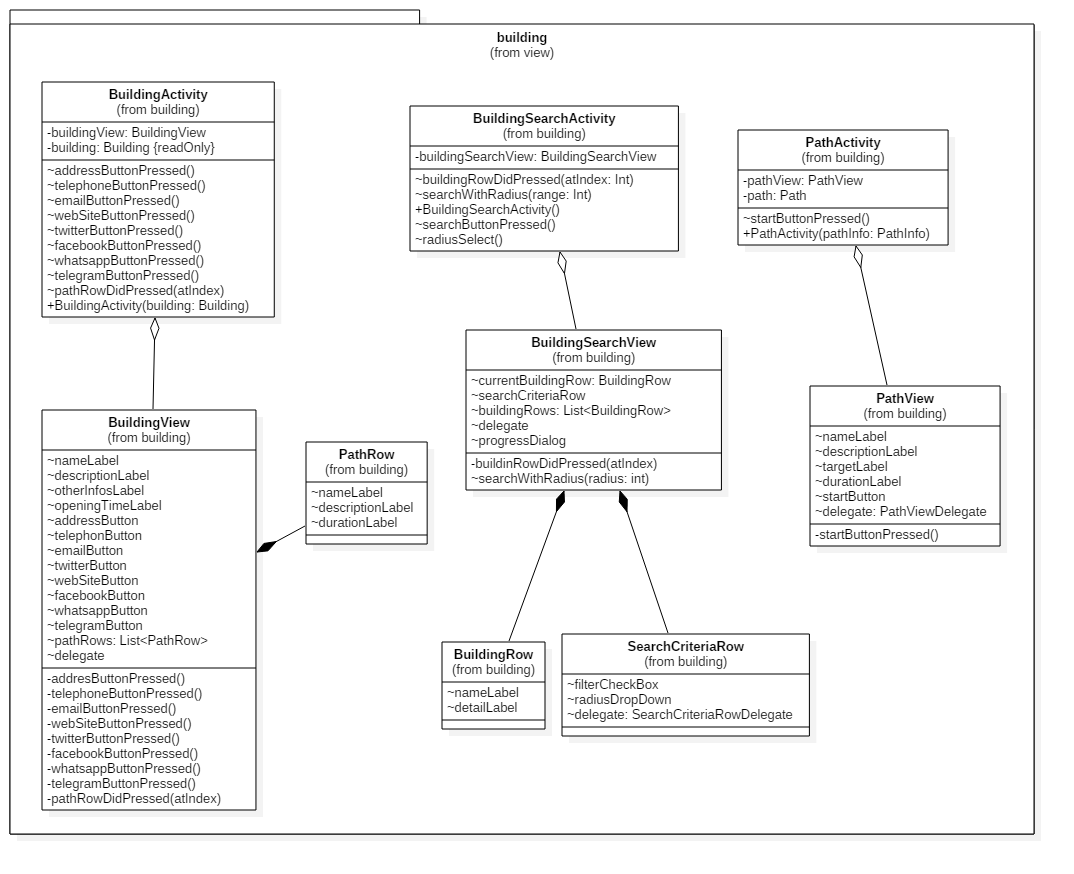
\includegraphics[scale=0.4]{img/package/png/client--viewcontroller--building.png}
\caption{Schema package client::viewcontroller::building}
 \end{figure}
\compDescrizione{componente che gestisce le informazioni e le interazioni dell'utente con gli edifici abilitati}
\compPadre{viewcontroller}
\begin{compClassi} \\
\begin{classe}{CLIPS::client::viewcontroller::building::BuildingActivity}
\classeDescrizione{classe controller che si occupa di interagire con BuildingView}
\classeUtilizzo{classe controller che si occupa di interagire con BuildingView}
\begin{classeMetodi}
\classeMetodo{onCreate}{savedInstanceState}{void}{si occupa di inizializzare l'activity con la relativa view}
\begin{classeMetodoArgomenti}
\classeMetodoArgomento{savedInstanceState}{Bundle}{contiene i dati dell'istanza creata o di un'attività precedente}
\end{classeMetodoArgomenti}
\classeMetodo{setButtons}{}{void}{si occupa di inizializzare i collegamenti dei bottoni presenti nella view
}
\classeMetodo{setItems}{}{void}{questo metodo rende cliccabile la lista dei risultati e rende visualizzabili i dettagli del percorso
selezionato}
\end{classeMetodi}
\begin{classeRelazioni}
\classeRelazione{CLIPS::client::viewcontroller::building}{BuildingView}{classe per la visualizzazione di un edificio}\end{classeRelazioni}
\end{classe}\begin{classe}{CLIPS::client::viewcontroller::building::BuildingRow}
\classeDescrizione{classe per la rappresentazione di un edificio nella ricerca}
\classeUtilizzo{permette di visualizzare le informazioni di un edificio nella lista dei risultati di ricerca}
\begin{classeAttributi}
\classeAttributo{detailLabel}{TextView}{rappresenta informazioni aggiuntive riguardanti l'edificio}
\classeAttributo{nameLabel}{TextView}{rappresenta il nome dell'edificio}
\end{classeAttributi}
\end{classe}\begin{classe}{CLIPS::client::viewcontroller::building::BuildingSearchActivity}
\classeDescrizione{classe controller che si occupa di interagire con BuildingSearchView}
\classeUtilizzo{si occupa di gestire le interazioni dell'utente con BuildingSearchView}
\begin{classeMetodi}
\classeMetodo{onCreate}{savedInstanceState}{void}{si occupa di inizializzare l'activity con la relativa view}
\begin{classeMetodoArgomenti}
\classeMetodoArgomento{savedInstanceState}{Bundle}{contiene i dati dell'istanza creata o di un'attività precedente}
\end{classeMetodoArgomenti}
\classeMetodo{setButtons}{}{void}{consente l'interazione con i bottoni presenti nella view}
\classeMetodo{setCheckBoxSignal}{}{void}{permette l'interazione per la selezione di ricerca per raggio}
\classeMetodo{setSeekBarSignal}{}{void}{permette di interagire con lo slider per impostare il raggio di ricerca}
\end{classeMetodi}
\begin{classeRelazioni}
\classeRelazione{CLIPS::client::viewcontroller::building}{BuildingSearchView}{classe per la ricerca degli edifici}\end{classeRelazioni}
\end{classe}\begin{classe}{CLIPS::client::viewcontroller::building::BuildingSearchView}
\classeDescrizione{classe per la ricerca degli edifici}
\classeUtilizzo{permette all'utente di cercare gli edifici vicini per visualizzare le informazioni e/o i percorsi disponibili}
\begin{classeAttributi}
\classeAttributo{buildingRows}{ListView}{indica la lista di edifici risultanti dalla ricerca}
\classeAttributo{searchCriteria}{SearchCriteriaRow}{indica i criteri di ricerca}
\end{classeAttributi}
\begin{classeRelazioni}
\classeRelazione{CLIPS::client::viewcontroller::building}{BuildingRow}{classe per la rappresentazione di un edificio nella ricerca}\classeRelazione{CLIPS::client::viewcontroller::building}{SearchCriteriaRow}{classe utilizzata per determinare i criteri di ricerca degli edifici}\end{classeRelazioni}
\end{classe}\begin{classe}{CLIPS::client::viewcontroller::building::BuildingView}
\classeDescrizione{classe per la visualizzazione di un edificio}
\classeUtilizzo{permette all'utente di visualizzare le informazioni relative all'edificio selezionato}
\begin{classeAttributi}
\classeAttributo{addressButton}{Button}{rappresenta l'indirizzo dell'edificio}
\classeAttributo{descriptionLabel}{TextView}{indica la descrizione dell'edificio}
\classeAttributo{emailButton}{Button}{indica l'indirizzo email dell'edificio}
\classeAttributo{facebookButton}{Button}{indica l'indirizzo facebook dell'edificio}
\classeAttributo{nameLabel}{TextView}{rappresenta il nome dell'edificio}
\classeAttributo{openingTimeLabel}{TextView}{rappresenta gli orari di apertura dell'edificio}
\classeAttributo{otherInfosLabel}{TextView}{rappresenta le altre informazioni sull'edificio}
\classeAttributo{pathRows}{List<TextView>}{rappresenta la lista dei percorsi dell'edificio}
\classeAttributo{telegramButton}{Button}{rappresenta il contatto Telegram dell'edificio}
\classeAttributo{telephoneButton}{Button}{rappresenta il numero telefonico dell'edificio}
\classeAttributo{twitterButton}{Button}{indica l'indirizzo twitter dell'edificio}
\classeAttributo{webSiteButton}{Button}{rappresenta l'indirizzo web dell'edificio}
\classeAttributo{whatsappButton}{Button}{indica il contatto WhatsApp dell'edificio}
\end{classeAttributi}
\begin{classeMetodi}
\classeMetodo{addressButtonPressed}{}{void}{notifica al controller l'interazione con addressButton}
\classeMetodo{emailButtonPressed}{}{void}{notifica al controller l'interazione con emailButton}
\classeMetodo{facebookButtonPressed}{}{void}{notifica al controller l'interazione con facebookButton}
\classeMetodo{pathRowDidPressed}{}{void}{notifica al controller l'interazione con pathRow}
\classeMetodo{telegramButtonPressed}{}{void}{notifica al controller l'interazione con telegramButton}
\classeMetodo{telephoneButtonPressed}{}{void}{notifica al controller l'interazione con telephoneButton}
\classeMetodo{twitterButtonPressed}{}{void}{notifica al controller l'interazione con twitterButton}
\classeMetodo{websiteButtonPressed}{}{void}{notifica al controller l'interazione con webSiteButton}
\classeMetodo{whatstappButtonPressed}{}{void}{notifica al controller l'interazione con whatsappButton}
\end{classeMetodi}
\begin{classeRelazioni}
\classeRelazione{CLIPS::client::viewcontroller::building}{PathRow}{classe per la rappresentazione di un percorso nella ricerca}\end{classeRelazioni}
\end{classe}\begin{classe}{CLIPS::client::viewcontroller::building::PathActivity}
\classeDescrizione{classe controller che si occupa di interagire con PathView}
\classeUtilizzo{si occupa di gestire le interazioni dell'utente con PathView}
\begin{classeMetodi}
\classeMetodo{onCreate}{savedInstanceState}{void}{si occupa di inizializzare l'activity con la relativa view}
\begin{classeMetodoArgomenti}
\classeMetodoArgomento{savedInstanceState}{Bundle}{contiene i dati dell'istanza creata o di un'attività precedente}
\end{classeMetodoArgomenti}
\end{classeMetodi}
\begin{classeRelazioni}
\classeRelazione{CLIPS::client::viewcontroller::building}{PathView}{classe che si occupa della visualizzazione della schermata riguardante un percorso}\end{classeRelazioni}
\end{classe}\begin{classe}{CLIPS::client::viewcontroller::building::PathRow}
\classeDescrizione{classe per la rappresentazione di un percorso nella ricerca}
\classeUtilizzo{permette un percorso disponibile nella lista dei risultati di ricerca}
\begin{classeAttributi}
\classeAttributo{pathName}{TextView}{contiene il nome del percorso}
\end{classeAttributi}
\end{classe}\begin{classe}{CLIPS::client::viewcontroller::building::PathView}
\classeDescrizione{classe che si occupa della visualizzazione della schermata riguardante un percorso}
\classeUtilizzo{consente all'utente di visualizzare le informazioni riguardanti un percorso e se l'utente si trova nell'edificio del percorso consente di iniziarlo}
\begin{classeAttributi}
\classeAttributo{descriptionLabel}{TextView}{rappresenta la descrizione del percorso}
\classeAttributo{durationLabel}{TextView}{rappresenta la durata stimata del percorso}
\classeAttributo{nameLabel}{TextView}{indica il nome del percorso}
\classeAttributo{startButton}{Button}{indica il bottone per iniziare il percorso}
\classeAttributo{targetLabel}{TextView}{indica a chi è consigliato questo percorso}
\end{classeAttributi}
\end{classe}\begin{classe}{CLIPS::client::viewcontroller::building::SearchCriteriaRow}
\classeDescrizione{classe utilizzata per determinare i criteri di ricerca degli edifici}
\classeUtilizzo{permette all'utente di visualizzare i criteri di ricerca disponibili}
\begin{classeAttributi}
\classeAttributo{distanceLabel}{TextView}{rappresenta la distanza selezionata nella ricerca per raggio}
\classeAttributo{filterCheckBox}{CheckBox}{viene usata per abilitare/disabilitare la ricerca per raggio}
\classeAttributo{kmFilter}{SeekBar}{indica i km da selezionare per la ricerca per raggio}
\classeAttributo{searchBuilding}{Button}{viene utilizzato per iniziare la ricerca degli edifici}
\end{classeAttributi}
\end{classe}\end{compClassi}
\end{componente}
\begin{componente}{CLIPS::client::viewcontroller::games}
\begin{figure}[h!]
	\centering
	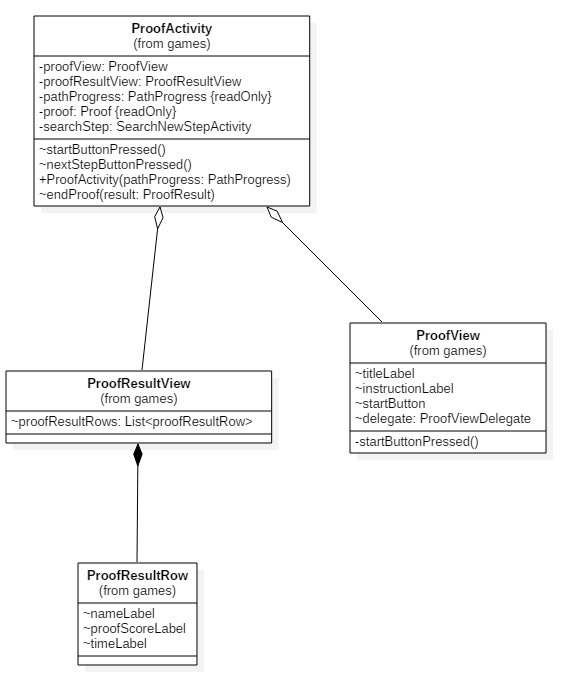
\includegraphics[scale=0.5]{img/package/png/client--viewcontroller--games1.png}
	\caption{Prima parte schema package client::viewcontroller::games}
\end{figure}
\begin{figure}[h!]
	\centering
	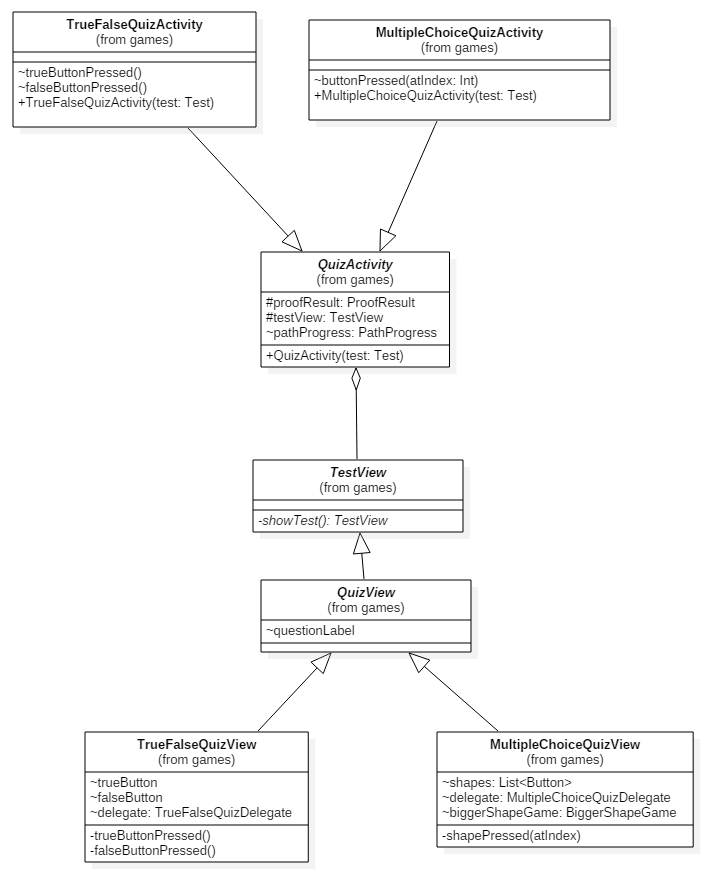
\includegraphics[scale=0.5]{img/package/png/client--viewcontroller--games2.png}
	\caption{Seconda parte schema package client::viewcontroller::games}
\end{figure}
\begin{figure}[h!]
	\centering
	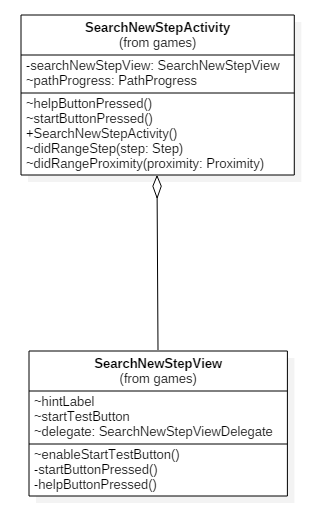
\includegraphics[scale=0.5]{img/package/png/client--viewcontroller--games3.png}
	\caption{Terza parte schema package client::viewcontroller::games}
\end{figure}
\compDescrizione{componente che gestisce le prove che l'utente deve completare all'interno di un percorso}
\compPadre{viewcontroller}
\begin{compClassi} \\
\begin{classe}{CLIPS::client::viewcontroller::games::MultipleChoiceQuizActivity}
\classeDescrizione{classe controller che si occupa di interagire con MultipleChoiceView}
\classeUtilizzo{si occupa di gestire le interazioni dell'utente con MultipleChoiceView}
\begin{classeMetodi}
\classeMetodo{onCreate}{}{void}{si occupa di inizializzare l'activity con la relativa view
}
\end{classeMetodi}
\begin{classeRelazioni}
\classeRelazione{CLIPS::client::viewcontroller::games}{QuizActivity}{interfaccia per segnalare gli eventi della classe QuizView}\end{classeRelazioni}
\end{classe}\begin{classe}{CLIPS::client::viewcontroller::games::MultipleChoiceQuizView}
\classeDescrizione{classe per il quiz a risposta multipla}
\classeUtilizzo{si occupa di fornire un'interfaccia per il quiz a risposta multipla}
\begin{classeAttributi}
\classeAttributo{choice1}{Button}{prima risposta alla domanda}
\classeAttributo{choice2}{Button}{seconda possibile risposta alla domanda}
\classeAttributo{choice3}{Button}{terza possibile risposta alla domanda}
\classeAttributo{choice4}{Button}{quarta possibile risposta alla domanda}
\end{classeAttributi}
\begin{classeRelazioni}
\classeRelazione{CLIPS::client::viewcontroller::games}{QuizView}{classe base per i quiz}\end{classeRelazioni}
\end{classe}\begin{classe}{CLIPS::client::viewcontroller::games::ProofActivity}
\classeDescrizione{classe controller che si occupa di interagire con ProofView}
\classeUtilizzo{si occupa di gestire le interazioni dell'utente con ProofView}
\begin{classeMetodi}
\classeMetodo{onCreate}{}{void}{si occupa di inizializzare l'activity con la relativa view}
\end{classeMetodi}
\begin{classeRelazioni}
\classeRelazione{CLIPS::client::viewcontroller::games}{ProofResultView}{classe che rappresenta la schermata dei risultati}\end{classeRelazioni}
\end{classe}\begin{classe}{CLIPS::client::viewcontroller::games::ProofResultActivity}
\classeDescrizione{classe che permette di visualizzare il risultato di una prova}
\classeUtilizzo{l'utente può vedere il risultato della prova che  ha appena svolto}
\begin{classeMetodi}
\classeMetodo{onCreate}{}{void}{si occupa di inizializzare l'activity con la relativa view}
\end{classeMetodi}
\end{classe}\begin{classe}{CLIPS::client::viewcontroller::games::ProofResultRow}
\classeDescrizione{classe che rappresenta una risultato rappresentato all'interno di una riga che può essere cliccata}
\classeUtilizzo{permette all'utente di visualizzare le informazioni generali di un risultato di una prova e di cliccarci per visualizzarne le informazioni dettagliate}
\end{classe}\begin{classe}{CLIPS::client::viewcontroller::games::ProofResultView}
\classeDescrizione{classe che rappresenta la schermata dei risultati}
\classeUtilizzo{permette all'utente di visualizzare le informazioni generali dei risultati delle prove e cliccare sulle prove delle quali vuole visualizzare le informazioni dettagliate}
\begin{classeAttributi}
\classeAttributo{result}{TextView}{contiene il risultato della prova appena svolta}
\end{classeAttributi}
\begin{classeRelazioni}
\classeRelazione{CLIPS::client::viewcontroller::games}{ProofResultRow}{classe che rappresenta una risultato rappresentato all'interno di una riga che può essere cliccata}\end{classeRelazioni}
\end{classe}\begin{classe}{CLIPS::client::viewcontroller::games::ProofView}
\classeDescrizione{classe che rappresenta la schermata della prova}
\classeUtilizzo{permette all'utente di visualizzare la prova da giocare}
\begin{classeAttributi}
\classeAttributo{instructionLabel}{TextView}{contiene le istruzioni relative alla prova}
\classeAttributo{startButton}{Button}{bottone che una volta premuto permette di iniziare la prova}
\end{classeAttributi}
\end{classe}\begin{classe}{CLIPS::client::viewcontroller::games::QuizActivity}
\classeDescrizione{interfaccia per segnalare gli eventi della classe QuizView}
\classeUtilizzo{si occupa di fornire i metodi necessari alla classe QuizView per notificare gli eventi}
\end{classe}\begin{classe}{CLIPS::client::viewcontroller::games::QuizResultView}
\classeDescrizione{classe per la visualizzazione del risultato di un quiz}
\classeUtilizzo{fornisce all'utente un'interfaccia affinché visualizzi il risultato del quiz}
\begin{classeAttributi}
\classeAttributo{continueButton}{Button}{button per chiudere la schermata e continuare il percorso}
\classeAttributo{feedbackLabel}{string}{mostra la frase di successo/fallimento del quiz}
\end{classeAttributi}
\begin{classeMetodi}
\classeMetodo{continueButtonPressed}{}{void}{notifica il controller che il button per continuare è stato premuto}
\classeMetodo{showFailureResult}{correctAnswer}{void}{mostra la risposta corretta se il quiz è stato fallito}
\begin{classeMetodoArgomenti}
\classeMetodoArgomento{correctAnswer}{string}{indica la risposta corretta}
\end{classeMetodoArgomenti}
\classeMetodo{showSuccessfulResult}{score}{void}{mostra il risultato ottenuto se il quiz è stato superato}
\begin{classeMetodoArgomenti}
\classeMetodoArgomento{score}{int}{indica il punteggio ottenuto}
\end{classeMetodoArgomenti}
\end{classeMetodi}
\end{classe}\begin{classe}{CLIPS::client::viewcontroller::games::QuizView}
\classeDescrizione{classe base per i quiz}
\classeUtilizzo{fornisce una base per i vari tipi di test da istanziare}
\begin{classeAttributi}
\classeAttributo{questionLabel}{string}{rappresenta la domanda da porre nel quiz}
\end{classeAttributi}
\begin{classeRelazioni}
\classeRelazione{CLIPS::client::viewcontroller::games}{TestView}{classe che fornisce una base dalla quale è possibile creare vari tipi di giochi }\end{classeRelazioni}
\end{classe}\begin{classe}{CLIPS::client::viewcontroller::games::SearchNewStepActivity}
\classeDescrizione{classe controller che si occupa di interagire con SearchNewStepView}
\classeUtilizzo{si occupa di gestire le interazioni dell'utente con SearchNewStepView}
\begin{classeMetodi}
\classeMetodo{onCreate}{savedInstanceState}{void}{si occupa di inizializzare l'activity con la relativa view}
\begin{classeMetodoArgomenti}
\classeMetodoArgomento{savedInstanceState}{Bundle}{stato dell'istanza}
\end{classeMetodoArgomenti}
\end{classeMetodi}
\begin{classeRelazioni}
\classeRelazione{CLIPS::client::viewcontroller::games}{SearchNewStepView}{classe che rappresenta la schermata per la ricerca della prossima prova del percorso}\end{classeRelazioni}
\end{classe}\begin{classe}{CLIPS::client::viewcontroller::games::SearchNewStepView}
\classeDescrizione{classe che rappresenta la schermata per la ricerca della prossima prova del percorso}
\classeUtilizzo{permette all'utente di cercare in modo semplificato la ricerca della prossima prova del percorso}
\begin{classeAttributi}
\classeAttributo{descriptionlabel}{TextView}{invita ad andare verso la prossima prova}
\classeAttributo{hintlabel}{TextView}{contiene il suggerimento per cercare la prossima prova}
\end{classeAttributi}
\end{classe}\begin{classe}{CLIPS::client::viewcontroller::games::TestResultView}
\classeDescrizione{classe che fornisce una base per la visualizzazione del risultato della prova}
\classeUtilizzo{permette all'utente di visualizzare il risultato della prova}
\begin{classeMetodi}
\classeMetodo{showResult}{}{void}{restituisce la view con il risultato}
\end{classeMetodi}
\end{classe}\begin{classe}{CLIPS::client::viewcontroller::games::TestView}
\classeDescrizione{classe che fornisce una base dalla quale è possibile creare vari tipi di giochi }
\classeUtilizzo{viene utilizzata per visualizzare un'interfaccia di gioco all'utente}
\begin{classeMetodi}
\classeMetodo{showTest}{}{TestView}{restituisce l'interfaccia grafica del test}
\end{classeMetodi}
\end{classe}\begin{classe}{CLIPS::client::viewcontroller::games::TrueFalseQuizActivity}
\classeDescrizione{classe controller che si occupa di interagire con TrueFalseQuizView}
\classeUtilizzo{si occupa di gestire le interazioni dell'utente con TrueFalseQuizView}
\begin{classeMetodi}
\classeMetodo{onCreate}{savedInstanceState}{void}{si occupa di inizializzare l'activity con la relativa view}
\begin{classeMetodoArgomenti}
\classeMetodoArgomento{savedInstanceState}{Bundle}{stato dell'istanza}
\end{classeMetodoArgomenti}
\end{classeMetodi}
\begin{classeRelazioni}
\classeRelazione{CLIPS::client::viewcontroller::games}{QuizActivity}{interfaccia per segnalare gli eventi della classe QuizView}\end{classeRelazioni}
\end{classe}\begin{classe}{CLIPS::client::viewcontroller::games::TrueFalseQuizView}
\classeDescrizione{classe per il quiz vero/falso}
\classeUtilizzo{si occupa di fornire un'interfaccia per la prova di tipo vero/falso}
\begin{classeAttributi}
\classeAttributo{falseButton}{Button}{button grafico per rispondere falso al quiz}
\classeAttributo{trueButton}{Button}{button grafico per rispondere vero al quiz}
\end{classeAttributi}
\begin{classeMetodi}
\classeMetodo{falseButtonPressed}{}{void}{questo metodo si occupa di notificare al controller che è stato premuto falseButton}
\classeMetodo{trueButtonPressed}{}{void}{questo metodo si occupa di notificare al controller che è stato premuto trueButton}
\end{classeMetodi}
\begin{classeRelazioni}
\classeRelazione{CLIPS::client::viewcontroller::games}{QuizView}{classe base per i quiz}\end{classeRelazioni}
\end{classe}\end{compClassi}
\end{componente}
\begin{componente}{CLIPS::client::viewcontroller::savedresults}
\begin{figure}[h!]
\centering
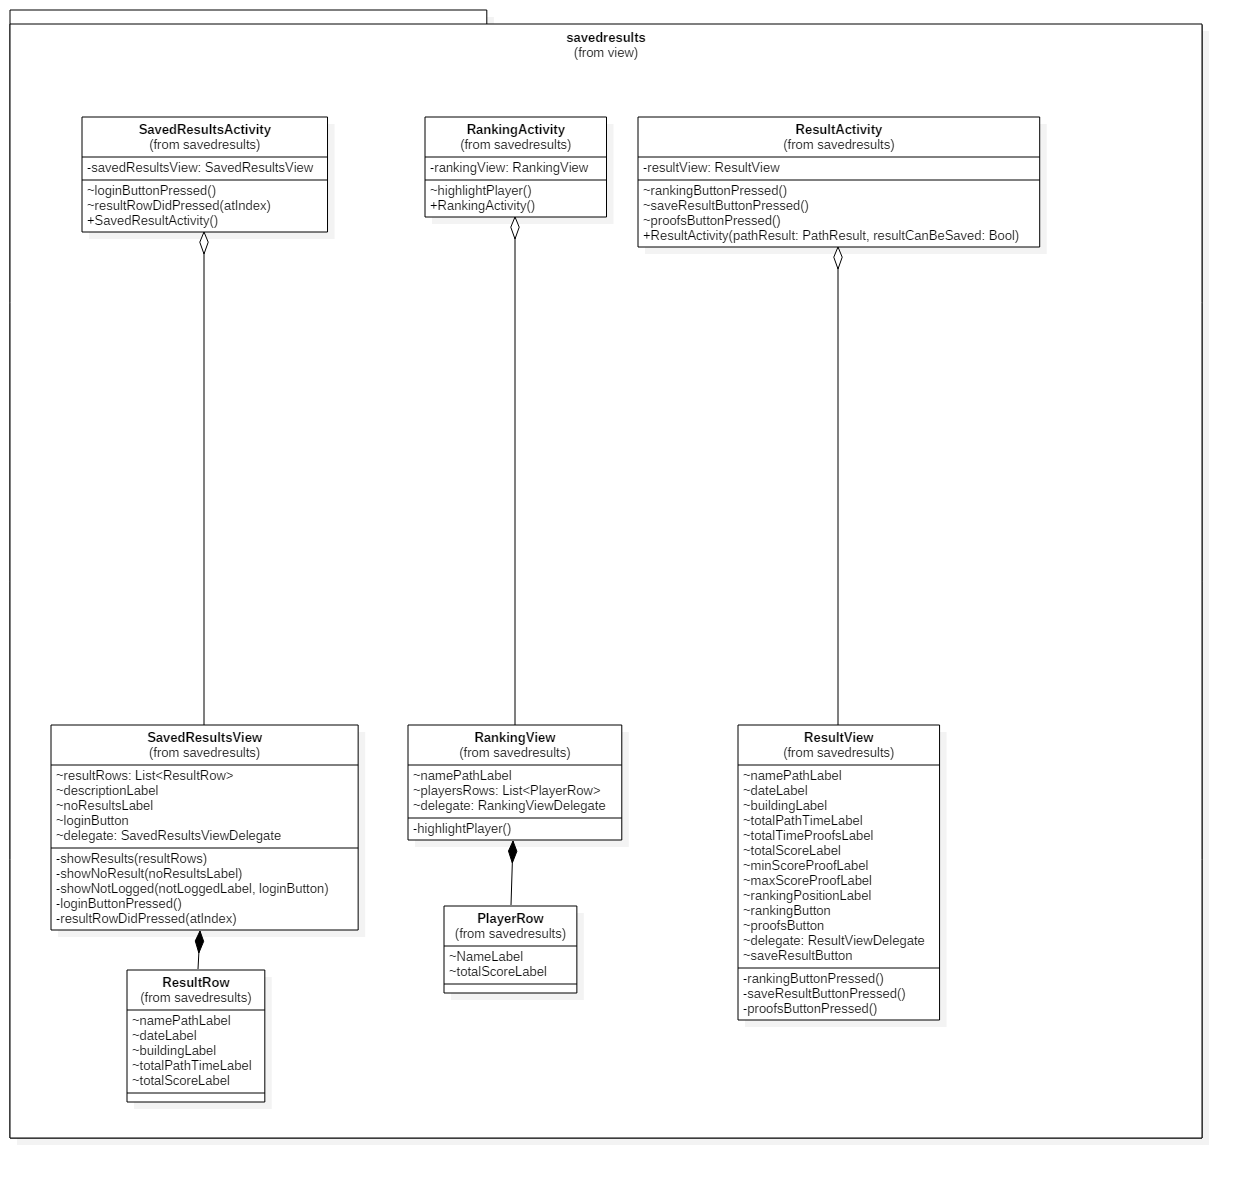
\includegraphics[scale=0.4]{img/package/png/client--viewcontroller--savedresults.png}
\caption{Schema package client::viewcontroller::savedresults}
 \end{figure}
\compDescrizione{componente che raggruppa le le view e i controller dei risultati salvati e delle classifiche}
\compPadre{viewcontroller}
\begin{compClassi} \\
\begin{classe}{CLIPS::client::viewcontroller::savedresults::PlayerRow}
\classeDescrizione{classe che rappresenta una riga all'interno di una classifica}
\classeUtilizzo{permette all'utente di visualizzare il nome del giocatore e il suo punteggio nel percorso d'interesse}
\begin{classeAttributi}
\classeAttributo{nameLabel}{TextView}{indica il nome del giocatore}
\classeAttributo{totalScoreLabel}{TextView}{indica il punteggio conseguito dal giocatore}
\end{classeAttributi}
\end{classe}\begin{classe}{CLIPS::client::viewcontroller::savedresults::RankingActivity}
\classeDescrizione{classe controller che si occupa di interagire con RankingView}
\classeUtilizzo{si occupa di gestire le interazioni dell'utente con RankingView}
\begin{classeMetodi}
\classeMetodo{onCreate}{savedInstanceState}{void}{si occupa di inizializzare l'activity con la relativa view}
\begin{classeMetodoArgomenti}
\classeMetodoArgomento{savedInstanceState}{Bundle}{contiene i dati dell'istanza creata o di un'attività precedente}
\end{classeMetodoArgomenti}
\end{classeMetodi}
\end{classe}\begin{classe}{CLIPS::client::viewcontroller::savedresults::RankingView}
\classeDescrizione{classe per rappresentare la classifica di un percorso}
\classeUtilizzo{permette all'utente di visualizzare la classifica del percorso}
\begin{classeAttributi}
\classeAttributo{namePathLabel}{TextView}{indica il nome del percorso}
\classeAttributo{playerRows}{ListView}{rappresenta la lista dei giocatori in classifica}
\end{classeAttributi}
\begin{classeRelazioni}
\classeRelazione{CLIPS::client::viewcontroller::savedresults}{RankingActivity}{classe controller che si occupa di interagire con RankingView}\end{classeRelazioni}
\end{classe}\begin{classe}{CLIPS::client::viewcontroller::savedresults::ResultActivity}
\classeDescrizione{classe controller che si occupa di interagire con ResultView}
\classeUtilizzo{si occupa di gestire le interazioni dell'utente con ResultView}
\begin{classeMetodi}
\classeMetodo{onCreate}{}{void}{si occupa di inizializzare l'activity con la relativa view}
\end{classeMetodi}
\begin{classeRelazioni}
\classeRelazione{CLIPS::client::viewcontroller::savedresults}{ResultView}{classe che rappresenta la schermata nel quali si possono visualizzare i risultati di un percorso}\classeRelazione{CLIPS::client::viewcontroller::savedresults}{ResultView}{classe che rappresenta la schermata nel quali si possono visualizzare i risultati di un percorso}\end{classeRelazioni}
\end{classe}\begin{classe}{CLIPS::client::viewcontroller::savedresults::ResultRow}
\classeDescrizione{classe che rappresenta una riga di un risultato}
\classeUtilizzo{permette all'utente di visualizzare le informazioni generali di un risultato e di cliccarci per visualizzare quelle dettagliate}
\begin{classeAttributi}
\classeAttributo{buildingLabel}{TextView}{rappresenta l'edificio dove si è svolto il percorso}
\classeAttributo{dateLabel}{TextView}{indica la data del percorso}
\classeAttributo{namePathLabel}{TextView}{indica il nome del percorso}
\classeAttributo{totalPathTimeLabel}{TextView}{indica il tempo totale speso per completare percorso}
\classeAttributo{totalScoreLabel}{TextView}{rappresenta il punteggio totale ottenuto svolgendo il percorso}
\end{classeAttributi}
\end{classe}\begin{classe}{CLIPS::client::viewcontroller::savedresults::ResultView}
\classeDescrizione{classe che rappresenta la schermata nel quali si possono visualizzare i risultati di un percorso}
\classeUtilizzo{permette all'utente di visualizzare le informazioni dettagliate del risultato di un percorso}
\begin{classeAttributi}
\classeAttributo{buildingLabel}{TextView}{rappresenta il nome dell'edificio dove si è svolto il percorso}
\classeAttributo{dateLabel}{TextView}{indica la data in cui si è svolto il percorso}
\classeAttributo{maxScoreProofLabel}{TextView}{rappresenta il punteggio massimo conseguito in una prova}
\classeAttributo{minScoreProofLabel}{TextView}{rappresenta il punteggio minimo conseguito in una prova}
\classeAttributo{namePathLabel}{TextView}{indica il nome del percorso}
\classeAttributo{proofsButton}{Button}{rappresenta il button delle prove}
\classeAttributo{rankingButton}{Button}{rappresenta il button per la classifica}
\classeAttributo{rankingPositionLabel}{TextView}{indica la posizione in classifica}
\classeAttributo{saveResultButton}{Button}{indica il bottone per salvare i risultati del percorso}
\classeAttributo{totalPathTimeLabel}{TextView}{indica il tempo totale speso per finire il percorso}
\classeAttributo{totalScoreLabel}{TextView}{indica il punteggio totale conseguito}
\classeAttributo{totalTimeProofsLabel}{TextView}{rappresenta il tempo totale impiegato per le prove del percorso}
\end{classeAttributi}
\end{classe}\begin{classe}{CLIPS::client::viewcontroller::savedresults::SavedResultsActivity}
\classeDescrizione{classe controller che si occupa di interagire con SavedResultView}
\classeUtilizzo{si occupa di gestire le interazioni dell'utente con SavedResultView}
\begin{classeMetodi}
\classeMetodo{isLoggedIn}{}{bool}{controlla se l'utente è loggiato per poter visualizzare i suoi risultati}
\classeMetodo{onCreate}{}{void}{si occupa di inizializzare l'activity con la relativa view}
\classeMetodo{setButtons}{}{void}{si occupa di impostare i collegamenti dei bottoni presenti nella view}
\end{classeMetodi}
\begin{classeRelazioni}
\classeRelazione{CLIPS::client::viewcontroller::savedresults}{SavedResultView}{classe che rappresenta la schermata dei risultati salvati di un utente}\end{classeRelazioni}
\end{classe}\begin{classe}{CLIPS::client::viewcontroller::savedresults::SavedResultView}
\classeDescrizione{classe che rappresenta la schermata dei risultati salvati di un utente}
\classeUtilizzo{permette all'utente di visualizzare i propri risultati salvati}
\begin{classeAttributi}
\classeAttributo{descriptionLabel}{TextView}{rappresenta la descrizione del percorso}
\classeAttributo{loginButton}{Button}{rappresenta il button per effettuare il login}
\classeAttributo{noResultsLabel}{TextView}{indica se non è presente nessun risultato}
\classeAttributo{resultRows}{ListView}{indica la lista di risultati}
\end{classeAttributi}
\begin{classeRelazioni}
\classeRelazione{CLIPS::client::viewcontroller::savedresults}{ResultRow}{classe che rappresenta una riga di un risultato}\end{classeRelazioni}
\end{classe}\end{compClassi}
\end{componente}
\begin{componente}{CLIPS::client::viewcontroller::utility}
\begin{figure}[h!]
\centering
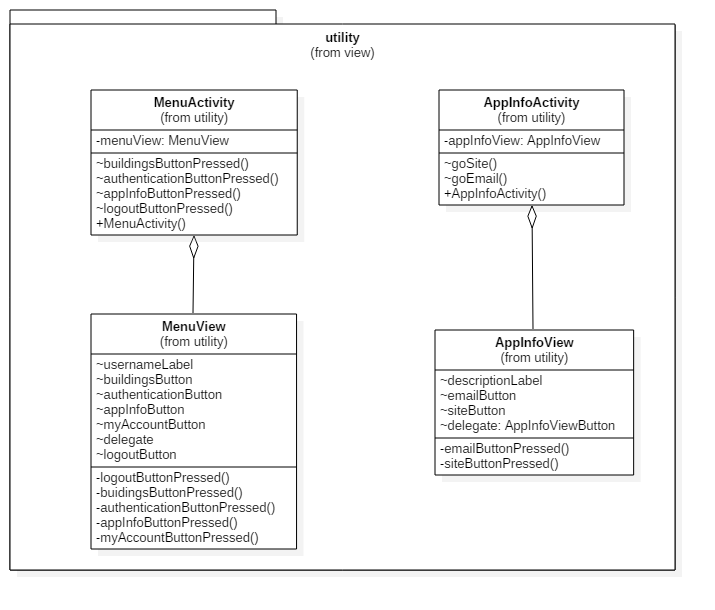
\includegraphics[scale=0.4]{img/package/png/client--viewcontroller--utility.png}
\caption{Schema package client::viewcontroller::utility}
 \end{figure}
\compDescrizione{componente che raggruppa le view generali dell'app}
\compPadre{viewcontroller}
\begin{compClassi} \\
\begin{classe}{CLIPS::client::viewcontroller::utility::AppInfoActivity}
\classeDescrizione{classe controller che si occupa di interagire con AppInfoView}
\classeUtilizzo{si occupa di gestire le interazioni dell'utente con AppInfoView}
\begin{classeMetodi}
\classeMetodo{onCreate}{savedInstanceState}{void}{si occupa di inizializzare l'activity con la relativa view}
\begin{classeMetodoArgomenti}
\classeMetodoArgomento{savedInstanceState}{Bundle}{stato dell'istanza}
\end{classeMetodoArgomenti}
\end{classeMetodi}
\begin{classeRelazioni}
\classeRelazione{CLIPS::client::viewcontroller::utility}{AppInfoView}{classe che si occupa delle informazioni generali dell'app}\end{classeRelazioni}
\end{classe}\begin{classe}{CLIPS::client::viewcontroller::utility::AppInfoView}
\classeDescrizione{classe che si occupa delle informazioni generali dell'app}
\classeUtilizzo{permette all'utente di visualizzare le informazioni generali dell'app}
\begin{classeAttributi}
\classeAttributo{textContainer}{LinearLayout}{layout che contiene le TextView necessarie a descrivere le informazioni dell'app}
\end{classeAttributi}
\end{classe}\begin{classe}{CLIPS::client::viewcontroller::utility::MenuActivity}
\classeDescrizione{classe controller che si occupa di interagire con MenuView}
\classeUtilizzo{si occupa di gestire le interazioni dell'utente con MenuView}
\begin{classeMetodi}
\classeMetodo{selectDrawerItem}{}{void}{si occupa di gestire i bottoni presenti nel menu}
\classeMetodo{setContentView}{layoutResID}{void}{si occupa di gestire gli elementi del layout della classe }
\begin{classeMetodoArgomenti}
\classeMetodoArgomento{layoutResID}{int}{layout da inserire}
\end{classeMetodoArgomenti}
\classeMetodo{setupContent}{}{void}{si occupa di impostare il contenuto della classe}
\classeMetodo{useDrawerToggle}{}{bool}{ritorna true se si intende utilizzare il drawer toggle, false altrimenti}
\classeMetodo{useToolbar}{}{bool}{ritorna true se si intende utilizzare la toolbar, false altrimenti}
\end{classeMetodi}
\begin{classeRelazioni}
\classeRelazione{CLIPS::client::viewcontroller::utility}{MenuView}{classe che si occupa di far visualizzare il menu}\end{classeRelazioni}
\end{classe}\begin{classe}{CLIPS::client::viewcontroller::utility::MenuView}
\classeDescrizione{classe che si occupa di far visualizzare il menu}
\classeUtilizzo{consente all'utente di navigare nell'app tramite il menu}
\end{classe}\end{compClassi}
\end{componente}
\begin{componente}{CLIPS::server}
\begin{figure}[h!]
\centering
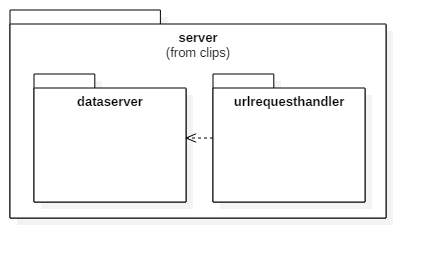
\includegraphics[scale=0.4]{img/package/png/server.png}
\caption{Schema package server}
 \end{figure}
\compDescrizione{componente globale per il back end del prodotto}
\compPadre{CLIPS}
\begin{compPackageContenuti}
\item \texttt{CLIPS::server::dataserver}: package per la gestione dei dati sul server
\item \texttt{CLIPS::server::urlrequesthandler}: componente che gestisce le richieste inviate al server e le risposte da inviare al client
\end{compPackageContenuti}
\end{componente}
\begin{componente}{CLIPS::server::dataserver}
\begin{figure}[h!]
\centering
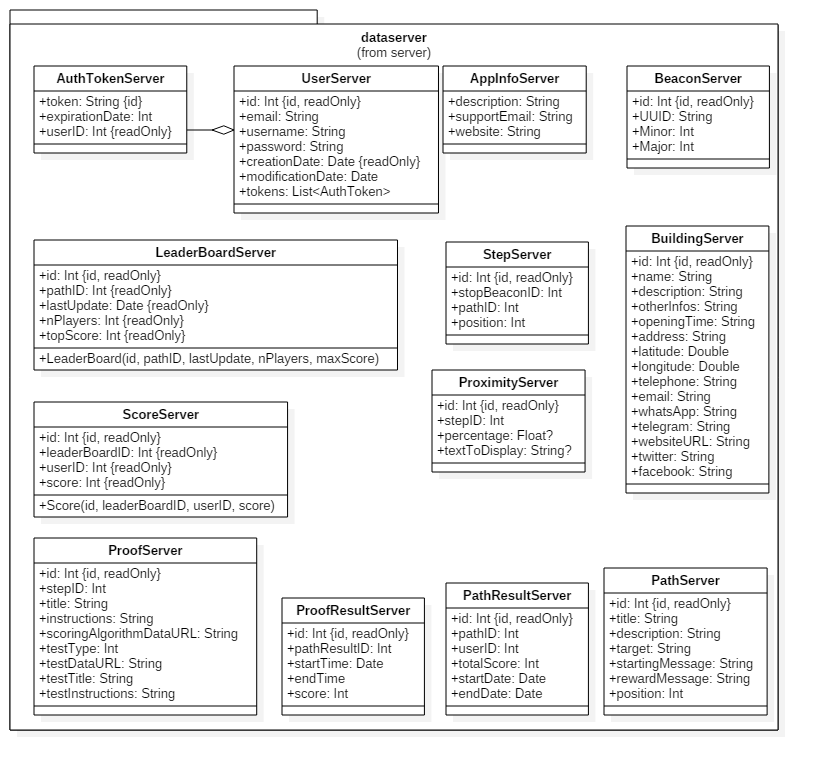
\includegraphics[scale=0.4]{img/package/png/server--data.png}
\caption{Schema package server::dataserver}
 \end{figure}
\compDescrizione{package per la gestione dei dati sul server}
\compPadre{server}
\begin{compClassi} \\
\begin{classe}{CLIPS::server::dataserver::AppInfo}
\classeDescrizione{classe che rappresenta le informazioni dell'app sul server}
\classeUtilizzo{permette di salvare sul server le informazioni dell'app}
\end{classe}\begin{classe}{CLIPS::server::dataserver::AuthToken}
\classeDescrizione{Classe che rappresenta un token che si riferisce ad un utente loggato}
\classeUtilizzo{permette utilizzare un token per riferirsi ad utente loggato}
\end{classe}\begin{classe}{CLIPS::server::dataserver::Beacon}
\classeDescrizione{classe che rappresenta un beacon nel server}
\classeUtilizzo{permette di salvare sul server un beacon}
\end{classe}\begin{classe}{CLIPS::server::dataserver::Building}
\classeDescrizione{classe che rappresenta un edificio sul server}
\classeUtilizzo{permette di salvare e modificare i dati di un edificio sul server}
\end{classe}\begin{classe}{CLIPS::server::dataserver::LeaderBoard}
\classeDescrizione{classe che rappresenta la classifica sul server}
\classeUtilizzo{permette di salvare i dati della classifica sul server}
\end{classe}\begin{classe}{CLIPS::server::dataserver::PathResult}
\classeDescrizione{classe che rappresenta il risultato di un percorso sul server}
\classeUtilizzo{consente di salvare i risultati di un percorso sul server}
\end{classe}\begin{classe}{CLIPS::server::dataserver::Path}
\classeDescrizione{classe che rappresenta un percorso sul server}
\classeUtilizzo{permette di creare, modificare ed eliminare un percorso sul server}
\end{classe}\begin{classe}{CLIPS::server::dataserver::ProofResult}
\classeDescrizione{classe che rappresenta i risultati di una prova sul server}
\classeUtilizzo{consente di salvare il risultato di una prova sul server}
\end{classe}\begin{classe}{CLIPS::server::dataserver::Proof}
\classeDescrizione{classe che rappresenta una prova sul server}
\classeUtilizzo{permette di creare, modificare ed eliminare una prova sul server}
\end{classe}\begin{classe}{CLIPS::server::dataserver::Proximity}
\classeDescrizione{classe che rappresenta sul server un beacon indicato alla segnalazione della distanza dalla prossima prova}
\classeUtilizzo{permette di salvare i beacon di segnalazione sul server}
\end{classe}\begin{classe}{CLIPS::server::dataserver::ScoreManager}
\classeDescrizione{classe che rappresenta un risultato sul server}
\classeUtilizzo{permette si salvare un risultato nel server}
\end{classe}\begin{classe}{CLIPS::server::dataserver::Step}
\classeDescrizione{classe che rappresenta uno step di un percorso nel server}
\classeUtilizzo{permette di salvare sul server uno step di un percorso}
\end{classe}\begin{classe}{CLIPS::server::dataserver::User}
\classeDescrizione{classe che rappresenta un utente nel server}
\classeUtilizzo{permette di salvare sul server un utente}
\begin{classeRelazioni}
\classeRelazione{CLIPS::server::dataserver}{AuthToken}{Classe che rappresenta un token che si riferisce ad un utente loggato}\end{classeRelazioni}
\end{classe}\end{compClassi}
\end{componente}
\begin{componente}{CLIPS::server::urlrequesthandler}
\begin{figure}[h!]
\centering
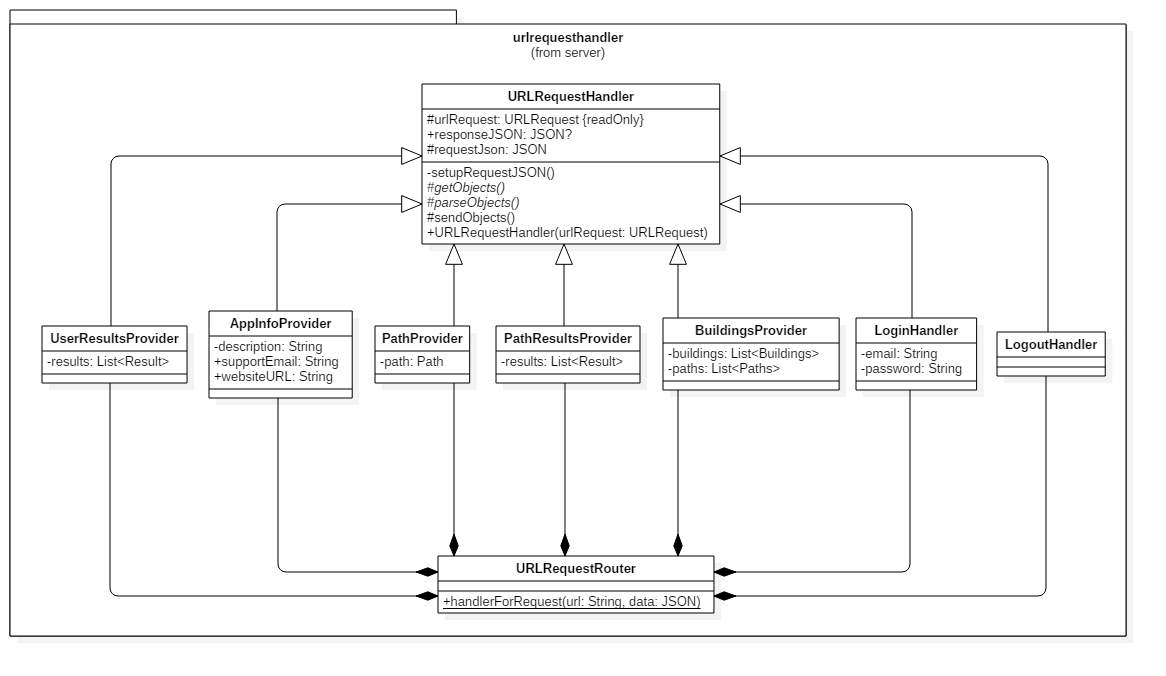
\includegraphics[scale=0.4]{img/package/png/server--urlrequesthandler.png}
\caption{Schema package server::urlrequesthandler}
 \end{figure}
\compDescrizione{componente che gestisce le richieste inviate al server e le risposte da inviare al client}
\compPadre{server}
\begin{compClassi} \\
\begin{classe}{CLIPS::server::urlrequesthandler::AppInfoProvider}
\classeDescrizione{classe che gestisce la richiesta di informazioni sull'app (come la descrizione dell'app, l'indirizzo del sito di supporto, l'email del supporto tecnico ed altro)}
\classeUtilizzo{si occupa di restituire le informazioni dell'app richieste}
\end{classe}\begin{classe}{CLIPS::server::urlrequesthandler::BuildingsProvider}
\classeDescrizione{classe che gestisce la richiesta degli edifici dal client al server}
\classeUtilizzo{si occupa di restituire le informazioni sugli edifici richieste}
\begin{classeMetodi}
\classeMetodo{addDistance}{}{void}{aggiunge ad un edificio la distanza dal client}
\classeMetodo{addPAthToBuildings}{buildings}{Promise}{ritorna una Promise che aggiunge le descrizioni dei percorsi agli edifici in input}
\begin{classeMetodoArgomenti}
\classeMetodoArgomento{buildings}{JSON}{array di edifici cui si vogliono aggiungere le descrizioni dei percorsi}
\end{classeMetodoArgomenti}
\end{classeMetodi}
\begin{classeRelazioni}
\classeRelazione{CLIPS::server::urlrequesthandler}{DBHandler}{classe che si occupa di gestire il DB e di ritornare un oggetto configurato della libreria knex}\end{classeRelazioni}
\end{classe}\begin{classe}{CLIPS::server::urlrequesthandler::DBHandler}
\classeDescrizione{classe che si occupa di gestire il DB e di ritornare un oggetto configurato della libreria knex}
\classeUtilizzo{creando un oggetto di questa classe è possibile creare query per interagire con il database}
\begin{classeMetodi}
\classeMetodo{getDB}{}{JSON}{ritorna un oggetto database di knex che si può interrogare per ottenere o inserire dati nel database}
\end{classeMetodi}
\end{classe}\begin{classe}{CLIPS::server::urlrequesthandler::EmailChecker}
\classeDescrizione{fornisce i metodi per la validazione di un indirizzo email}
\classeUtilizzo{attraverso il metodo isValid(string) è possibile controllare se l'indirizzo email passato in input è valido}
\begin{classeMetodi}
\classeMetodo{isValid}{email}{bool}{ritorna vero se l'indirizzo mail è valido}
\begin{classeMetodoArgomenti}
\classeMetodoArgomento{email}{string}{email che si intende validare verificare}
\end{classeMetodoArgomenti}
\end{classeMetodi}
\end{classe}\begin{classe}{CLIPS::server::urlrequesthandler::LoginHandler}
\classeDescrizione{classe che gestisce le richieste di login da parte del client}
\classeUtilizzo{si occupa di gestire il login lato server}
\begin{classeMetodi}
\classeMetodo{userID}{password}{Promise}{ritorna una Promise che ottiene in maniera asincrona l'id dell'utente se la coppia email/password è valida, un messaggio di errore altrimenti}
\begin{classeMetodoArgomenti}
\classeMetodoArgomento{password}{string}{password dell'utente che intende autenticarsi}
\end{classeMetodoArgomenti}
\end{classeMetodi}
\begin{classeRelazioni}
\classeRelazione{CLIPS::server::urlrequesthandler}{DBHandler}{classe che si occupa di gestire il DB e di ritornare un oggetto configurato della libreria knex}\end{classeRelazioni}
\end{classe}\begin{classe}{CLIPS::server::urlrequesthandler::LogoutHandler}
\classeDescrizione{classe che gestisce la richiesta di logout da parte del client (eliminando il token associato al client)}
\classeUtilizzo{si occupa di effettuare il logout lato server}
\end{classe}\begin{classe}{CLIPS::server::urlrequesthandler::PasswordChecker}
\classeDescrizione{verifica che la password soddisfi i requisiti minimi di sicurezza}
\classeUtilizzo{utilizzare il metodo isValid(string) per verificare la sicurezza sufficiente della password inserita}
\begin{classeAttributi}
\classeAttributo{instructions}{string}{istruzioni da far visualizzare all'utente per fornire una password valida}
\end{classeAttributi}
\begin{classeMetodi}
\classeMetodo{isValid}{password}{bool}{ritorna vero se la password è valida}
\begin{classeMetodoArgomenti}
\classeMetodoArgomento{password}{string}{la password che si intende verificare}
\end{classeMetodoArgomenti}
\end{classeMetodi}
\end{classe}\begin{classe}{CLIPS::server::urlrequesthandler::PathProvider}
\classeDescrizione{classe che gestisce la richiesta del percorso dal client}
\classeUtilizzo{si occupa di restituire le informazioni sul percorso richieste}
\begin{classeMetodi}
\classeMetodo{fulfilledProof}{proof}{Promise}{ritorna una Promise in grado di aggiungere in maniera asincrona i dati derivati alla prova in ingresso}
\begin{classeMetodoArgomenti}
\classeMetodoArgomento{proof}{JSON}{la prova che si vuole completare inserendo dati derivati}
\end{classeMetodoArgomenti}
\classeMetodo{fulfilledProximity}{proximity}{Promise}{ritorna una Promise in grado di aggiungere in maniera asincrona i dati derivati alla Proximity in ingresso}
\begin{classeMetodoArgomenti}
\classeMetodoArgomento{proximity}{JSON}{la Proximity che si vuole completare inserendo dati derivati}
\end{classeMetodoArgomenti}
\classeMetodo{fulfilledStep}{step}{Promise}{ritorna una Promise in grado di aggiungere in maniera asincrona i dati derivati alla tappe in ingresso}
\begin{classeMetodoArgomenti}
\classeMetodoArgomento{step}{JSON}{la tappa che si vuole completare inserendo dati derivati}
\end{classeMetodoArgomenti}
\classeMetodo{getAlgorithm}{proof}{Promise}{ritorna una Promise in grado di tornare l'algoritmo per il calcolo dei punteggi della prova in input}
\begin{classeMetodoArgomenti}
\classeMetodoArgomento{proof}{JSON}{la prova di cui si vuole ottenere l'algoritmo}
\end{classeMetodoArgomenti}
\classeMetodo{getBeacon}{beaconID}{Promise}{metodo che ritorna una Promise in grado di recuperare in maniera asincrona i dati di un Beacon con ID in ingresso}
\begin{classeMetodoArgomenti}
\classeMetodoArgomento{beaconID}{int}{ID del beacon di cui si vogliono recuperare le informazioni}
\end{classeMetodoArgomenti}
\classeMetodo{getPath}{pathID}{Promise}{ritorna una Promise in grado di recuperare in maniera asincrona i dati del percorso associate all'ID in ingresso}
\begin{classeMetodoArgomenti}
\classeMetodoArgomento{pathID}{int}{id del percorso di cui si vogliono recuperare i dati}
\end{classeMetodoArgomenti}
\classeMetodo{getProof}{step}{Promise}{metodo che ritorna una Promise in grado di recuperare in maniera asincrona i dati della prova associata alla tappa in ingresso}
\begin{classeMetodoArgomenti}
\classeMetodoArgomento{step}{JSON}{tappa di cui si vogliono recuperare i dati relativi alla prova}
\end{classeMetodoArgomenti}
\classeMetodo{getProximities}{step}{Promise}{ritorna una Promise in grado di recuperare in maniera asincrona i dati delle Proximity associate alla tappa in ingresso}
\begin{classeMetodoArgomenti}
\classeMetodoArgomento{step}{JSON}{tappa di cui si vogliono avere le proximities}
\end{classeMetodoArgomenti}
\classeMetodo{getSteps}{path}{Promise}{metodo che ritorna una Promise in grado di recuperare in maniera asincrona i dati delle tappe associate al path in ingresso}
\begin{classeMetodoArgomenti}
\classeMetodoArgomento{path}{JSON}{path di cui si vogliono avere le tappe}
\end{classeMetodoArgomenti}
\classeMetodo{getTest}{proof}{Promise}{ritorna una Promise in grado di ottenere i dati relativi ai giochi nella prova da effettuare}
\begin{classeMetodoArgomenti}
\classeMetodoArgomento{proof}{JSON}{la prova di cui si vogliono ottenere i dati}
\end{classeMetodoArgomenti}
\end{classeMetodi}
\begin{classeRelazioni}
\classeRelazione{CLIPS::server::urlrequesthandler}{DBHandler}{classe che si occupa di gestire il DB e di ritornare un oggetto configurato della libreria knex}\end{classeRelazioni}
\end{classe}\begin{classe}{CLIPS::server::urlrequesthandler::PathResultsProvider}
\classeDescrizione{classe che gestisce la richiesta del risultato del percorso dal client}
\classeUtilizzo{si occupa di restituire le informazioni del risultato sul percorso richieste}
\begin{classeRelazioni}
\classeRelazione{CLIPS::server::urlrequesthandler}{DBHandler}{classe che si occupa di gestire il DB e di ritornare un oggetto configurato della libreria knex}\end{classeRelazioni}
\end{classe}\begin{classe}{CLIPS::server::urlrequesthandler::RegistrationFieldsValidator}
\classeDescrizione{classe del server che si occupa di validare i dati di registrazione}
\classeUtilizzo{la classe presenta un metodo execute che verifica la richiesta effettuata dal client e quali sono i dati forniti e risponde con le indicazioni di quali sono campi validi}
\begin{classeRelazioni}
\classeRelazione{CLIPS::server::urlrequesthandler}{EmailChecker}{fornisce i metodi per la validazione di un indirizzo email}\classeRelazione{CLIPS::server::urlrequesthandler}{PasswordChecker}{verifica che la password soddisfi i requisiti minimi di sicurezza}\classeRelazione{CLIPS::server::urlrequesthandler}{UsernameChecker}{si occupa di verificare la validità dell'username (in particolare se è già in uso da un utente)}\end{classeRelazioni}
\end{classe}\begin{classe}{CLIPS::server::urlrequesthandler::RegistrationHandler}
\classeDescrizione{classe che si occupa di registrare i nuovi utenti}
\classeUtilizzo{è necessario impostare gli attributi response e request e successivamente chiamare il metodo execute()}
\end{classe}\begin{classe}{CLIPS::server::urlrequesthandler::URLRequestHandler}
\classeDescrizione{classe astratta che rappresenta un gestore di richieste di dati fatte al server}
\classeUtilizzo{si occupa di gestire le richieste ricevute dal client}
\begin{classeAttributi}
\classeAttributo{request}{HTTP.Request}{richiesta http effettuata da un client}
\classeAttributo{response}{HTTP.Response}{risposta che il server invia al client}
\end{classeAttributi}
\begin{classeMetodi}
\classeMetodo{execute}{}{void}{prende in carico la richiesta, ne studia i parametri in ingresso e invia al client la risposta}
\end{classeMetodi}
\end{classe}\begin{classe}{CLIPS::server::urlrequesthandler::URLRequestRouter}
\classeDescrizione{classe che si occupa di creare il corretto URLRequestHandler per gestire la richiesta HTTP rivolta al server}
\classeUtilizzo{crea la classe URLRequestHandler appropriata}
\begin{classeRelazioni}
\classeRelazione{CLIPS::server::urlrequesthandler}{AppInfoProvider}{classe che gestisce la richiesta di informazioni sull'app (come la descrizione dell'app, l'indirizzo del sito di supporto, l'email del supporto tecnico ed altro)}\classeRelazione{CLIPS::server::urlrequesthandler}{BuildingsProvider}{classe che gestisce la richiesta degli edifici dal client al server}\classeRelazione{CLIPS::server::urlrequesthandler}{LoginHandler}{classe che gestisce le richieste di login da parte del client}\classeRelazione{CLIPS::server::urlrequesthandler}{LogoutHandler}{classe che gestisce la richiesta di logout da parte del client (eliminando il token associato al client)}\classeRelazione{CLIPS::server::urlrequesthandler}{PathProvider}{classe che gestisce la richiesta del percorso dal client}\classeRelazione{CLIPS::server::urlrequesthandler}{PathResultsProvider}{classe che gestisce la richiesta del risultato del percorso dal client}\classeRelazione{CLIPS::server::urlrequesthandler}{RegistrationFieldsValidator}{classe del server che si occupa di validare i dati di registrazione}\classeRelazione{CLIPS::server::urlrequesthandler}{UserResultProvider}{classe che gestisce la richiesta di un utente}\end{classeRelazioni}
\end{classe}\begin{classe}{CLIPS::server::urlrequesthandler::UsernameChecker}
\classeDescrizione{si occupa di verificare la validità dell'username (in particolare se è già in uso da un utente)}
\classeUtilizzo{è utile per verificare che un username non sia ancora stato utilizzato}
\end{classe}\begin{classe}{CLIPS::server::urlrequesthandler::UserResultProvider}
\classeDescrizione{classe che gestisce la richiesta di un utente}
\classeUtilizzo{si occupa di restituire gli utenti richiesti dal client}
\end{classe}\end{compClassi}
\end{componente}
